% Generated by Sphinx.
\def\sphinxdocclass{report}
\documentclass[a4paper,10pt,icelandic]{sphinxmanual}
\usepackage[utf8]{inputenc}
\DeclareUnicodeCharacter{00A0}{\nobreakspace}
\usepackage{cmap}
\usepackage[T1]{fontenc}
\usepackage{babel}
\usepackage{times}
\usepackage[Sonny]{fncychap}
\usepackage{longtable}
\usepackage{sphinx}
\usepackage{multirow}


\usepackage{amsmath}
\usepackage{amssymb}
\usepackage{hyperref}


\title{Stærðfræðigreining II (STÆ205G)}
\release{2017}
\author{Sigurður Örn Stefánsson}
\newcommand{\sphinxlogo}{
\includegraphics{hi_horiz_raunvisindadeild.png}\par}
\renewcommand{\releasename}{Útgáfa}
\makeindex

\makeatletter
\def\PYG@reset{\let\PYG@it=\relax \let\PYG@bf=\relax%
    \let\PYG@ul=\relax \let\PYG@tc=\relax%
    \let\PYG@bc=\relax \let\PYG@ff=\relax}
\def\PYG@tok#1{\csname PYG@tok@#1\endcsname}
\def\PYG@toks#1+{\ifx\relax#1\empty\else%
    \PYG@tok{#1}\expandafter\PYG@toks\fi}
\def\PYG@do#1{\PYG@bc{\PYG@tc{\PYG@ul{%
    \PYG@it{\PYG@bf{\PYG@ff{#1}}}}}}}
\def\PYG#1#2{\PYG@reset\PYG@toks#1+\relax+\PYG@do{#2}}

\expandafter\def\csname PYG@tok@gt\endcsname{\def\PYG@tc##1{\textcolor[rgb]{0.00,0.27,0.87}{##1}}}
\expandafter\def\csname PYG@tok@sc\endcsname{\def\PYG@tc##1{\textcolor[rgb]{0.25,0.44,0.63}{##1}}}
\expandafter\def\csname PYG@tok@gh\endcsname{\let\PYG@bf=\textbf\def\PYG@tc##1{\textcolor[rgb]{0.00,0.00,0.50}{##1}}}
\expandafter\def\csname PYG@tok@sd\endcsname{\let\PYG@it=\textit\def\PYG@tc##1{\textcolor[rgb]{0.25,0.44,0.63}{##1}}}
\expandafter\def\csname PYG@tok@sr\endcsname{\def\PYG@tc##1{\textcolor[rgb]{0.14,0.33,0.53}{##1}}}
\expandafter\def\csname PYG@tok@gi\endcsname{\def\PYG@tc##1{\textcolor[rgb]{0.00,0.63,0.00}{##1}}}
\expandafter\def\csname PYG@tok@ow\endcsname{\let\PYG@bf=\textbf\def\PYG@tc##1{\textcolor[rgb]{0.00,0.44,0.13}{##1}}}
\expandafter\def\csname PYG@tok@nn\endcsname{\let\PYG@bf=\textbf\def\PYG@tc##1{\textcolor[rgb]{0.05,0.52,0.71}{##1}}}
\expandafter\def\csname PYG@tok@mo\endcsname{\def\PYG@tc##1{\textcolor[rgb]{0.13,0.50,0.31}{##1}}}
\expandafter\def\csname PYG@tok@mi\endcsname{\def\PYG@tc##1{\textcolor[rgb]{0.13,0.50,0.31}{##1}}}
\expandafter\def\csname PYG@tok@mf\endcsname{\def\PYG@tc##1{\textcolor[rgb]{0.13,0.50,0.31}{##1}}}
\expandafter\def\csname PYG@tok@kt\endcsname{\def\PYG@tc##1{\textcolor[rgb]{0.56,0.13,0.00}{##1}}}
\expandafter\def\csname PYG@tok@gs\endcsname{\let\PYG@bf=\textbf}
\expandafter\def\csname PYG@tok@ne\endcsname{\def\PYG@tc##1{\textcolor[rgb]{0.00,0.44,0.13}{##1}}}
\expandafter\def\csname PYG@tok@gp\endcsname{\let\PYG@bf=\textbf\def\PYG@tc##1{\textcolor[rgb]{0.78,0.36,0.04}{##1}}}
\expandafter\def\csname PYG@tok@c1\endcsname{\let\PYG@it=\textit\def\PYG@tc##1{\textcolor[rgb]{0.25,0.50,0.56}{##1}}}
\expandafter\def\csname PYG@tok@kp\endcsname{\def\PYG@tc##1{\textcolor[rgb]{0.00,0.44,0.13}{##1}}}
\expandafter\def\csname PYG@tok@gu\endcsname{\let\PYG@bf=\textbf\def\PYG@tc##1{\textcolor[rgb]{0.50,0.00,0.50}{##1}}}
\expandafter\def\csname PYG@tok@w\endcsname{\def\PYG@tc##1{\textcolor[rgb]{0.73,0.73,0.73}{##1}}}
\expandafter\def\csname PYG@tok@o\endcsname{\def\PYG@tc##1{\textcolor[rgb]{0.40,0.40,0.40}{##1}}}
\expandafter\def\csname PYG@tok@ge\endcsname{\let\PYG@it=\textit}
\expandafter\def\csname PYG@tok@vg\endcsname{\def\PYG@tc##1{\textcolor[rgb]{0.73,0.38,0.84}{##1}}}
\expandafter\def\csname PYG@tok@na\endcsname{\def\PYG@tc##1{\textcolor[rgb]{0.25,0.44,0.63}{##1}}}
\expandafter\def\csname PYG@tok@gd\endcsname{\def\PYG@tc##1{\textcolor[rgb]{0.63,0.00,0.00}{##1}}}
\expandafter\def\csname PYG@tok@nt\endcsname{\let\PYG@bf=\textbf\def\PYG@tc##1{\textcolor[rgb]{0.02,0.16,0.45}{##1}}}
\expandafter\def\csname PYG@tok@c\endcsname{\let\PYG@it=\textit\def\PYG@tc##1{\textcolor[rgb]{0.25,0.50,0.56}{##1}}}
\expandafter\def\csname PYG@tok@kr\endcsname{\let\PYG@bf=\textbf\def\PYG@tc##1{\textcolor[rgb]{0.00,0.44,0.13}{##1}}}
\expandafter\def\csname PYG@tok@nl\endcsname{\let\PYG@bf=\textbf\def\PYG@tc##1{\textcolor[rgb]{0.00,0.13,0.44}{##1}}}
\expandafter\def\csname PYG@tok@nc\endcsname{\let\PYG@bf=\textbf\def\PYG@tc##1{\textcolor[rgb]{0.05,0.52,0.71}{##1}}}
\expandafter\def\csname PYG@tok@sb\endcsname{\def\PYG@tc##1{\textcolor[rgb]{0.25,0.44,0.63}{##1}}}
\expandafter\def\csname PYG@tok@kd\endcsname{\let\PYG@bf=\textbf\def\PYG@tc##1{\textcolor[rgb]{0.00,0.44,0.13}{##1}}}
\expandafter\def\csname PYG@tok@gr\endcsname{\def\PYG@tc##1{\textcolor[rgb]{1.00,0.00,0.00}{##1}}}
\expandafter\def\csname PYG@tok@err\endcsname{\def\PYG@bc##1{\setlength{\fboxsep}{0pt}\fcolorbox[rgb]{1.00,0.00,0.00}{1,1,1}{\strut ##1}}}
\expandafter\def\csname PYG@tok@vi\endcsname{\def\PYG@tc##1{\textcolor[rgb]{0.73,0.38,0.84}{##1}}}
\expandafter\def\csname PYG@tok@go\endcsname{\def\PYG@tc##1{\textcolor[rgb]{0.20,0.20,0.20}{##1}}}
\expandafter\def\csname PYG@tok@sx\endcsname{\def\PYG@tc##1{\textcolor[rgb]{0.78,0.36,0.04}{##1}}}
\expandafter\def\csname PYG@tok@m\endcsname{\def\PYG@tc##1{\textcolor[rgb]{0.13,0.50,0.31}{##1}}}
\expandafter\def\csname PYG@tok@no\endcsname{\def\PYG@tc##1{\textcolor[rgb]{0.38,0.68,0.84}{##1}}}
\expandafter\def\csname PYG@tok@bp\endcsname{\def\PYG@tc##1{\textcolor[rgb]{0.00,0.44,0.13}{##1}}}
\expandafter\def\csname PYG@tok@s1\endcsname{\def\PYG@tc##1{\textcolor[rgb]{0.25,0.44,0.63}{##1}}}
\expandafter\def\csname PYG@tok@cp\endcsname{\def\PYG@tc##1{\textcolor[rgb]{0.00,0.44,0.13}{##1}}}
\expandafter\def\csname PYG@tok@s\endcsname{\def\PYG@tc##1{\textcolor[rgb]{0.25,0.44,0.63}{##1}}}
\expandafter\def\csname PYG@tok@nf\endcsname{\def\PYG@tc##1{\textcolor[rgb]{0.02,0.16,0.49}{##1}}}
\expandafter\def\csname PYG@tok@ni\endcsname{\let\PYG@bf=\textbf\def\PYG@tc##1{\textcolor[rgb]{0.84,0.33,0.22}{##1}}}
\expandafter\def\csname PYG@tok@k\endcsname{\let\PYG@bf=\textbf\def\PYG@tc##1{\textcolor[rgb]{0.00,0.44,0.13}{##1}}}
\expandafter\def\csname PYG@tok@s2\endcsname{\def\PYG@tc##1{\textcolor[rgb]{0.25,0.44,0.63}{##1}}}
\expandafter\def\csname PYG@tok@nd\endcsname{\let\PYG@bf=\textbf\def\PYG@tc##1{\textcolor[rgb]{0.33,0.33,0.33}{##1}}}
\expandafter\def\csname PYG@tok@se\endcsname{\let\PYG@bf=\textbf\def\PYG@tc##1{\textcolor[rgb]{0.25,0.44,0.63}{##1}}}
\expandafter\def\csname PYG@tok@nv\endcsname{\def\PYG@tc##1{\textcolor[rgb]{0.73,0.38,0.84}{##1}}}
\expandafter\def\csname PYG@tok@cm\endcsname{\let\PYG@it=\textit\def\PYG@tc##1{\textcolor[rgb]{0.25,0.50,0.56}{##1}}}
\expandafter\def\csname PYG@tok@mh\endcsname{\def\PYG@tc##1{\textcolor[rgb]{0.13,0.50,0.31}{##1}}}
\expandafter\def\csname PYG@tok@si\endcsname{\let\PYG@it=\textit\def\PYG@tc##1{\textcolor[rgb]{0.44,0.63,0.82}{##1}}}
\expandafter\def\csname PYG@tok@kn\endcsname{\let\PYG@bf=\textbf\def\PYG@tc##1{\textcolor[rgb]{0.00,0.44,0.13}{##1}}}
\expandafter\def\csname PYG@tok@nb\endcsname{\def\PYG@tc##1{\textcolor[rgb]{0.00,0.44,0.13}{##1}}}
\expandafter\def\csname PYG@tok@ss\endcsname{\def\PYG@tc##1{\textcolor[rgb]{0.32,0.47,0.09}{##1}}}
\expandafter\def\csname PYG@tok@kc\endcsname{\let\PYG@bf=\textbf\def\PYG@tc##1{\textcolor[rgb]{0.00,0.44,0.13}{##1}}}
\expandafter\def\csname PYG@tok@il\endcsname{\def\PYG@tc##1{\textcolor[rgb]{0.13,0.50,0.31}{##1}}}
\expandafter\def\csname PYG@tok@cs\endcsname{\def\PYG@tc##1{\textcolor[rgb]{0.25,0.50,0.56}{##1}}\def\PYG@bc##1{\setlength{\fboxsep}{0pt}\colorbox[rgb]{1.00,0.94,0.94}{\strut ##1}}}
\expandafter\def\csname PYG@tok@vc\endcsname{\def\PYG@tc##1{\textcolor[rgb]{0.73,0.38,0.84}{##1}}}
\expandafter\def\csname PYG@tok@sh\endcsname{\def\PYG@tc##1{\textcolor[rgb]{0.25,0.44,0.63}{##1}}}

\def\PYGZbs{\char`\\}
\def\PYGZus{\char`\_}
\def\PYGZob{\char`\{}
\def\PYGZcb{\char`\}}
\def\PYGZca{\char`\^}
\def\PYGZam{\char`\&}
\def\PYGZlt{\char`\<}
\def\PYGZgt{\char`\>}
\def\PYGZsh{\char`\#}
\def\PYGZpc{\char`\%}
\def\PYGZdl{\char`\$}
\def\PYGZhy{\char`\-}
\def\PYGZsq{\char`\'}
\def\PYGZdq{\char`\"}
\def\PYGZti{\char`\~}
% for compatibility with earlier versions
\def\PYGZat{@}
\def\PYGZlb{[}
\def\PYGZrb{]}
\makeatother

\begin{document}

\maketitle
\tableofcontents
\phantomsection\label{index::doc}



\chapter*{Formáli}
\label{formali::doc}\label{formali:staerfraeigreining-ii-stae205g-haskoli-islands-vor-2016}\label{formali:formali}
Þetta kennsluefni er ætlað til að styðja við kennslu í áfanganum
Stærðfræðigreining II við Háskóla Íslands. Það er bæði aðgengilegt sem
vefsíða, \href{http://notendur.hi.is/sigurdur/stae205}{http://notendur.hi.is/sigurdur/stae205}, og sem \href{https://notendur.hi.is/sigurdur/stae205/stae205.pdf}{pdf-skjal} sem hentar
til útprentunar. Efnið byggir upprunalega á glærupakka sem \href{http://starfsfolk.hi.is/simaskra/1198}{Rögnvaldur
Möller} útbjó fyrir sambærilegan áfanga. Efnið er skrifað í
Markup-tungumáli í kerfinu Sphinx sem upphaflega var hannað fyrir
hjálpina í forritunarmálinu Python. \href{http://notendur.hi.is/bsm}{Benedikt Steinar Magnússon} aðlagaði kerfið þannig að það hentar til
að útbúa kennsluefni og naut við það aðstoðar Sólrúnar Höllu
Einarsdóttur. Kerfið er opið og allar viðbætur við það eru
aðgengilegar á \href{http://github.com/edbook}{http://github.com/edbook}. Arnbjörg Soffía Árnadóttir og
Þorsteinn Hjörtur Jónsson sáu um uppsetningu á efninu í
Stærðfræðigreiningu II og kann ég þeim bestu þakkir fyrir.

\textbf{Janúar 2016, Sigurður Örn Stefánsson}

Sumarið 2016 var þýðingu lykilorða bætt við kerfið. Símon Böðvarsson sá um forritunarvinnuna. Þýðingar eru sóttar úr \href{http://stæ.is/os}{Orðaskrá Íslenska stærðfræðafélagsins}. Þegar músabendill svífur yfir lykilorði birtist fyrsta þýðing þess samkvæmt orðaskránni. Í sumum tilfellum eru margar mögulegar þýðingar sem eiga misvel við en þá er hægt að smella á orðið til að sjá alla möguleika.

\textbf{Janúar 2017, Sigurður Örn Stefánsson}


\chapter*{Gagnlegar upplýsingar}
\label{umnamskeidid::doc}\label{umnamskeidid:gagnlegar-upplysingar}

\section*{Námsefnið}
\label{umnamskeidid:namsefni}
Viðfangsefnið eru varpanir sem skilgreindar eru á
hlutmengi í \(\mathbb{R}^n\) og taka gildi í \(\mathbb{R}^m\).  Sérstaklega munum við skoða
varpanir \(\mathbf{r}:[a,b]\rightarrow \mathbb{R}^m\) (stikaferla) og föll \(f:\mathbb{R}^n\rightarrow
\mathbb{R}\).  Námskeiðið skiptist í tvo svo til jafnstóra hluta þar sem í
öðrum er diffrun í aðalhlutverki og í hinum heildun.   Meginþema í
námskeiðinu er beiting á aðferðum stærðfræðigreiningar á rúmfræðileg
verkefni.

Þegar þið þurfið virkilega að reikna, hvort sem það er í námi eða
starfi,   er líklegt að reyni á kunnáttu ykkar í efni þessa
námskeiðs.

Notuð er sama kennslubók og í Stærðfræðigreiningu I, 8. útgáfa af
Calculus eftir Adams. Í námskeiðinu verður farið yfir mest allt efni kafla 8, 11,
12, 13, 14, 15 og 16 (sjá áætlun um fyrirlestra).


\section*{Fyrirlestrar}
\label{umnamskeidid:fyrirlestrar}
Fyrirlestrar verða 8:20-9:50 á mánudögum og 10:00-11:30 á
miðvikudögum.  Í fyrirlestraáætlun og  á
dæmablöðunum er sagt nánar frá efni fyrirlestra hverrar viku og
vísað á viðeigandi efnisgreinar í bók.  Helstu atriði
fyrirlestranna verða aðgengileg á vefnum.
Að mestu verður fylgt þeirri efnisröð sem er í bók Adams.


\section*{Dæmi og dæmatímar}
\label{umnamskeidid:daemi-og-daematimar}
Í tímunum 15:00-16:30 á mánudögum og 14:10-15:40 á þriðjudögum verða
reiknuð dæmi. Þið getið valið í hvorn tímann þið mætið. Rætt verður um lausnir skiladæma í tímanum 11:40-12:20 á miðvikudögum.

Því til viðbótar verða stoðtímar  á miðvikudögum og fimmtudögum.  Í þeim tímum gefst ykkur tækifæri á að fá aðstoð við skiladæmi og önnur dæmi sem þið eruð að glíma við og einnig að fá nánari útskýringar á atriðum úr fyrirlestrum og leystum dæmum. Þið getið valið í hvaða stoðtíma þið mætið en athugið að yfirleitt er mest álag í fimmtudagstímunum og því getur verið auðveldara að fá aðstoð fyrr í vikunni.

Dæmablöð og lausnir skiladæma verða settar á skráasvæðið í UGLU.

Í dæmatímum verður fyrst farið yfir dæmi með undirstrikuðum númerum.


\section*{Skiladæmi og próftökuréttur}
\label{umnamskeidid:skiladaemi-og-proftokurettur}
Á misserinu verða 11 sinnum lögð fyrir
skiladæmi. Fyrstu skiladæmi verða föstudaginn 13. janúar.

\begin{notice}{important}{Mikilvægt:}
Til að öðlast próftökurétt þarf að skila að minnsta kosti \textbf{7 af 11} heimadæmum. Skil teljast ekki gild nema þið hafi náð 50\% árangri í
glímunni við dæmin. Þið berið sjálf ábyrgð á að fylgjast með að skil séu rétt skráð í Uglunni. Yfirfarin heimadæmi undirrituð af
aðstoðarkennara gilda sem kvittun fyrir skilum. Haldið þeim því til haga!
\end{notice}

Dæmum á að skila fyrir 13:00 á föstudögum í \textbf{hólf merkt Sigurður Örn Stefánsson} í anddyri VRII.  Vinsamlegast merkið lausnir ykkar með \textbf{fullu nafni} ykkar og hvaða grein þið eruð í (t.d. rafmagnsverkfræði, efnafræði...)  \textbf{efst á fremstu síðunni}.  Ef lausnir ykkar eru á tveimur eða fleiri blöðum þá þurfið þið að hefta þau saman. Yfirfarnar úrlausnir má nálgast í rekkunum við stigann á jarðhæð í VRII á miðvikudagsmorgni vikuna eftir skil.


\section*{Próf}
\label{umnamskeidid:prof}
Á misserinu verða tvö stutt próf sem hvort um sig gildir 15\% til lokaeinkunnar en þó eingöngu til hækkunar.   Ég stefni að því að hafa fyrra prófið í tíma 22. febrúar.  Þá verður prófað úr lesnu efni, skilgreiningum og setningum.  Seinna prófið verður væntanlega í tíma 22. mars.  Á því prófi verða dæmi og atriði sem hafa komið fyrir í skiladæmum.  Engin skiladæmi eru lögð fyrir þær vikur sem prófin eru haldin.

Í lok námskeiðsins er þriggja tíma skriflegt próf sem gildir 70\%.  Nauðsynlegt og nægjanlegt er að fá a.m.k. 5 í lokaprófinu til að standast námskeiðið. Engin hjálpargögn eru heimil í prófinu, nema formúlublöð sem fylgja prófverkefni. Vasareiknar eru ekki leyfðir í prófinu. Á prófinu verða dæmi úr öllum hlutum námsefnisins.  Dæmin munu bæði reyna á reiknifærni og grundvallarskilning á hugtökum.


\section*{Að taka námskeiðið í annað sinn}
\label{umnamskeidid:a-taka-namskeii-i-anna-sinn}
Þau ykkar sem sátuð námskeiðið í fyrra og unnuð ykkur inn próftökurétt haldið próftökuréttinum en eldri próftökuréttur gildir ekki. Einkunnir úr misserisprófum frá í fyrra gilda ekki. Þið eruð hvött til að taka fullan þátt í námskeiðinu með dæmaskilum og þátttöku í misserisprófum.


\section*{Viðtalstímar kennara}
\label{umnamskeidid:vitalstimar-kennara}
Kennari námskeiðsins er Sigurður Örn Stefánsson, og hefur skrifstofu á þriðju hæð í Tæknigarði.  Tímarnir frá 11:40 - 12:20 á miðvikudögum verða nýttir til að fara yfir lausnir skiladæma og í fyrirspurnir og aðrar umræður. Aðrir viðtalstímar eru eftir samkomulagi.  Síminn minn er 525 5481 og tölvupóstfangið er \href{mailto:sigurdur@hi.is}{sigurdur@hi.is}.

\begin{notice}{important}{Mikilvægt:}
Þar sem mjög margir nemendur eru í námskeiðinu bið ég ykkur um að íhuga  áður en þið sendið tölvupóst hvort svarið við spurningunni
sé að finna í þessu skjali eða hvort þið gætuð borið spurninguna fram í fyrirlestri, dæmatíma, stoðtíma eða viðtalstíma.
\end{notice}


\section*{Hugbúnaður}
\label{umnamskeidid:hugbunaur}
Við munum nota forritið Matlab í námskeiðinu, aðallega til að framkalla teikningar. Á \href{http://notendur.hi.is/jonasson/matlab/}{heimasíðu Kristjáns Jónassonar} getið þið nálgast útgáfu af Matlab fyrir nemendur háskólans.

Fyrir þá sem kjósa frjálsan hugbúnað þá má benda á að forritið \href{http://www.gnu.org/software/octave}{Octave}, er að mestu leyti sambærilegt við Matlab.


\chapter{Ferlar}
\label{Kafli1::doc}\label{Kafli1:ferlar}
\emph{Winter is coming.}

- George R.R. Martin, A Game of Thrones


\section{Inngangur}
\label{Kafli1:inngangur}\begin{itemize}
\item {} 
Viðfangsefni námskeiðsins er varpanir sem skilgreindar eru á
hlutmengi í \(\mbox{${\bf R}^n$}\) og taka gildi í
\(\mbox{${\bf R}^m$}\).

\item {} 
Fáumst við stærðfræðigreiningu í mörgum breytistærðum.

\item {} 
Sambærileg verkefni og í stærðfræðigreiningu í einni breytistærð:
Samfelldni, diffrun, heildun. Rúmfræðileg túlkun skiptir nú miklu
máli.

\item {} 
Gerir okkur kleift að fást við mörg raunveruleg verkefni þar sem
margar breytistærðir koma við sögu.

\end{itemize}


\section{Stikaferlar}
\label{Kafli1:stikaferlar}
\index{vigurgild vörpun}\index{stikaferill}

\subsection{Skilgreining}
\label{Kafli1:skilgreining}\label{Kafli1:index-0}
Vörpun \(\mbox{${\bf r}$}:  [a,b]\rightarrow \mbox{${\bf R}^n$}\)
þannig að \(\mbox{${\bf r}$}(t)=(r_1(t),\ldots,r_n(t))\) kallast
\emph{vigurgild vörpun}. Slík vörpun er sögð samfelld ef föllin
\(r_1, \ldots, r_n\) eru öll samfelld. Samfelld vörpun
\(\mbox{${\bf r}$}:  [a,b]\rightarrow \mbox{${\bf R}^n$}\) er oft
kölluð \textit{stikaferill}.


\subsection{Ritháttur}
\label{Kafli1:rithattur}
Þegar fjallað er um stikaferil
\(\mbox{${\bf r}$}:  [a,b]\rightarrow {\mathbb  R}^2\) þá er oft
ritað
\begin{gather}
\begin{split}\displaystyle \mbox{${\bf r}$}=\mbox{${\bf r}$}(t)=(x(t),y(t))=x(t)\mbox{${\bf i}$}+y(t)\mbox{${\bf j}$},\end{split}\notag
\end{gather}
og þegar fjallað er um stikaferil
\(\mbox{${\bf r}$}:  [a,b]\rightarrow {\mathbb  R}^3\) þá er oft
ritað
\begin{gather}
\begin{split}\displaystyle \mbox{${\bf r}$}=\mbox{${\bf r}$}(t)=(x(t),y(t),z(t))=x(t)\mbox{${\bf i}$}+y(t)\mbox{${\bf j}$}+z(t)\mbox{${\bf k}$}.\end{split}\notag
\end{gather}

\section{Ferlar og stikanir á ferlum}
\label{Kafli1:ferlar-og-stikanir-a-ferlum}
\index{ferill}\index{stikun}

\subsection{Skilgreining}
\label{Kafli1:id1}\label{Kafli1:index-1}
\textit{Ferill í plani} er mengi punkta \((x,y)\) í planinu þannig að
skrifa má \(x=f(t)\) og \(y=g(t)\) fyrir \(t\) á bili
\(I\) þar sem \(f\) og \(g\) eru samfelld föll á \(I\).
Bilið \(I\) ásamt föllunum \((f,g)\) kallast \emph{s}tikun á
ferlinum. Ferill í rúmi og \textit{stikun} á ferli í rúmi eru skilgreind á
sambærilegan hátt.

\begin{notice}{warning}{Aðvörun:}
Ferill í plani/rúmi er \textbf{ekki} það sama og stikaferill. Fyrir gefinn
feril eru til (óendanlega) margar ólíkar stikanir.
\end{notice}


\subsection{Dæmi - Eðlisfræðileg túlkun}
\label{Kafli1:daemi-elisfraeileg-tulkun}
Líta má á veginn milli Reykjavíkur og Akureyrar sem feril.

Líta má á ferðalag eftir veginum frá Reykjavík til Akureyrar þar sem
staðsetning er þekkt á hverjum tíma sem stikaferil þar sem tíminn er
stikinn.


\subsection{Dæmi}
\label{Kafli1:daemi}
Jafnan
\begin{gather}
\begin{split}\displaystyle x^2+y^2 = 1\end{split}\notag
\end{gather}
lýsir ferli í planinu sem er hringur með miðju í (0,0) og geisla 1. Dæmi
um ólíkar stikanir:
\begin{gather}
\begin{split}\displaystyle\end{split}\notag\\\begin{split}\begin{aligned}
\mbox{${\bf r}$}_1(t) &= (\cos(t),\sin(t)), \quad \text{fyrir $t$ á bilinu $[0,2\pi].$} \\
\mbox{${\bf r}$}_2(t) &= \left\{\begin{array}{ll}
(t,\sqrt{1-t^2}) & \text{fyrir $t$ á bilinu $[-1,1[,$} \\
(2-t,-\sqrt{1-(2-t)^2}) & \text{fyrir $t$ á bilinu $[1,3].$}
\end{array}\right.\end{aligned}\end{split}\notag
\end{gather}


\section{Diffrun stikaferla}
\label{Kafli1:diffrun-stikaferla}
\index{stikaferill!diffrun}

\subsection{Skilgreining}
\label{Kafli1:id2}\label{Kafli1:index-2}
Stikaferill
\(\mbox{${\bf r}$}:  [a,b]\rightarrow \mbox{${\bf R}^n$}\) er
\emph{diffranlegur í punkti} \(t\) ef markgildið
\begin{gather}
\begin{split}\displaystyle \mbox{${\bf r}$}'(t)=\lim_{\Delta t\rightarrow 0}\frac{\mbox{${\bf r}$}(t+\Delta t)-\mbox{${\bf r}$}(t)}{\Delta t}\end{split}\notag
\end{gather}
er til. Stikaferillinn \(\mbox{${\bf r}$}\) er sagður \emph{diffranlegur}
ef hann er diffranlegur í öllum punktum á bilinu \([a,b]\). (Í
endapunktum bilsins \([a,b]\) er þess krafist að einhliða afleiður
séu skilgreindar.)


\subsection{Setning}
\label{Kafli1:setning}
Stikaferill
\(\mbox{${\bf r}$}:  [a,b]\rightarrow \mbox{${\bf R}^n$}\) er
\emph{diffranlegur í punkti} \(t\) ef og aðeins ef föllin
\(r_1,\ldots,r_n\) eru öll diffranleg í \(t\). Þá gildir að
\begin{gather}
\begin{split}\displaystyle \mbox{${\bf r}$}'(t)=(r'_1(t),\ldots,r'_n(t)).\end{split}\notag
\end{gather}
\index{hraðavigur}\index{hraði}\index{hröðunarvigur}\index{ferð}

\subsection{Ritháttur}
\label{Kafli1:index-3}\label{Kafli1:id3}
Látum \(\mbox{${\bf r}$}:  [a,b]\rightarrow \mbox{${\bf R}^n$}\)
vera diffranlegan stikaferil. Venja er að rita
\(\mbox{${\bf v}$}(t)=\mbox{${\bf r}$}'(t)\) og tala um
\(\mbox{${\bf v}$}(t)\) sem \textit{hraða} eða \emph{hraðavigur}. Talan
\(|\mbox{${\bf v}$}(t)|\) er kölluð \textit{ferð}. Einnig er ritað
\(\mbox{${\bf a}$}(t)=\mbox{${\bf v}$}'(t)=\mbox{${\bf r}$}''(t)\)
og talað um \(\mbox{${\bf a}$}(t)\) sem \textit{hröðun} eða
\emph{hröðunarvigur}.


\begin{center}
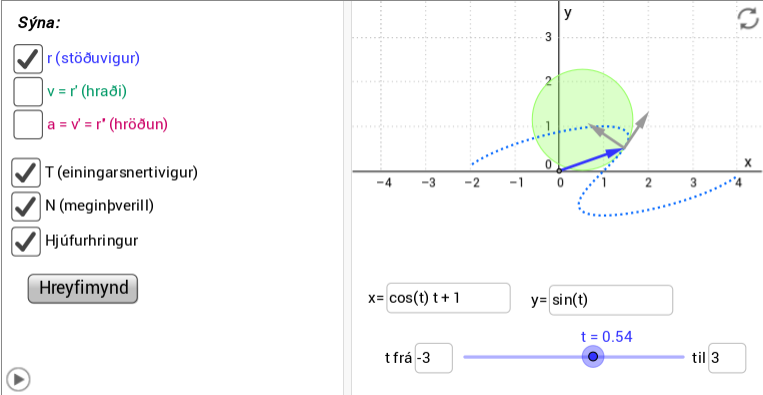
\includegraphics[width=10cm,keepaspectratio=true]{stikaferill.png}
\end{center}



\subsection{Dæmi}
\label{Kafli1:id4}
Lítum á eftirfarand stikaferla sem stika hring með miðju í (0,0) og
geisla 1.
\begin{gather}
\begin{split}\displaystyle\end{split}\notag\\\begin{split}\begin{aligned}
\mbox{${\bf r}$}_1(t) &= (\cos(t),\sin(t)), \quad \text{fyrir $t$ á bilinu $[0,2\pi].$} \\
\mbox{${\bf r}$}_2(t) &= (\cos(t^2),\sin(t^2)), \quad \text{fyrir $t$ á bilinu $[0,\sqrt{2\pi}].$} \end{aligned}\end{split}\notag
\end{gather}
Þá er tilsvarandi hraði
\begin{gather}
\begin{split}\displaystyle\end{split}\notag\\\begin{split}\begin{aligned}
\mbox{${\bf v}$}_1(t) = \mbox{${\bf r}$}_1'(t) &= (-\sin(t),\cos(t)), \quad \text{fyrir $t$ á bilinu $[0,2\pi].$} \\
\mbox{${\bf v}$}_2(t) = \mbox{${\bf r}$}_2'(t) &= (-2t\sin(t^2),2t\cos(t^2)),  \quad \text{fyrir $t$ á bilinu $[0,\sqrt{2\pi}].$}\end{aligned}\end{split}\notag
\end{gather}
og ferðin \(|\mbox{${\bf v}$}_1(t)| = 1\) og
\(|\mbox{${\bf v}$}_2(t)| = 2t\).


\subsection{Setning}
\label{Kafli1:id5}
Látum
\(\mbox{${\bf u}$},\mbox{${\bf v}$}:[a,b]\rightarrow \mbox{${\bf R}^n$}\)
vera diffranlega stikaferla og \(\lambda\) diffranlegt fall. Þá eru
stikaferlarnir
\(\mbox{${\bf u}$}(t)+\mbox{${\bf v}$}(t), \lambda(t)\mbox{${\bf u}$}(t)\)
og \(\mbox{${\bf u}$}(\lambda(t))\) diffranlegir, og ef \(n=3\)
þá er stikaferillinn
\(\mbox{${\bf u}$}(t)\times \mbox{${\bf v}$}(t)\) líka diffranlegur.
Fallið \(\mbox{${\bf u}$}(t)\cdot\mbox{${\bf v}$}(t)\) er líka
diffranlegt. Eftirfarandi listi sýnir formúlur fyrir afleiðunum:

\textbf{(a)}
\(\frac{d}{dt}(\mbox{${\bf u}$}(t)+\mbox{${\bf v}$}(t))=\mbox{${\bf u}$}'(t)+\mbox{${\bf v}$}'(t)\),

\textbf{(b)}
\(\frac{d}{dt}(\lambda(t)\mbox{${\bf u}$}(t))=\lambda'(t)\mbox{${\bf u}$}(t)+\lambda(t)\mbox{${\bf u}$}'(t)\),

\textbf{(c)}
\(\frac{d}{dt}(\mbox{${\bf u}$}(t)\cdot\mbox{${\bf v}$}(t))=\mbox{${\bf u}$}'(t)\cdot\mbox{${\bf v}$}(t)+\mbox{${\bf u}$}(t)\cdot\mbox{${\bf v}$}'(t)\),

\textbf{(d)}
\(\frac{d}{dt}(\mbox{${\bf u}$}(t)\times\mbox{${\bf v}$}(t))=\mbox{${\bf u}$}'(t)\times\mbox{${\bf v}$}(t)+\mbox{${\bf u}$}(t)\times\mbox{${\bf v}$}'(t)\),

\textbf{(e)}
\(\frac{d}{dt}(\mbox{${\bf u}$}(\lambda(t)))=\mbox{${\bf u}$}'(\lambda(t))\lambda'(t)\).

Ef \(\mbox{${\bf u}$}(t)\neq\mbox{${\bf 0}$}\) þá er

\textbf{(f)}
\(\frac{d}{dt}|\mbox{${\bf u}$}(t)|=\frac{\mbox{${\bf u}$}(t)\cdot\mbox{${\bf u}$}'(t)}{|\mbox{${\bf u}$}(t)|}\).

\index{stikaferill!samfellt diffranlegur}\index{stikaferill!þjáll}

\subsection{Skilgreining}
\label{Kafli1:index-4}\label{Kafli1:id6}
Látum
\(\mbox{${\bf r}$}:  [a,b]\rightarrow \mbox{${\bf R}^n$}; \mbox{${\bf r}$}(t)=(r_1(t),\ldots,r_n(t))\)
vera stikaferil.

Stikaferillinn er sagður \textit{samfellt diffranlegur} ef föllin
\(r_1(t),\ldots,r_n(t)\) eru öll diffranleg og afleiður þeirra eru
samfelldar. Samfellt diffranlegur stikaferill er sagður \textit{þjáll}
ef \(\mbox{${\bf r}$}'(t)\neq\mbox{${\bf 0}$}\) fyrir
öll \(t\).

Stikaferillinn er sagður \emph{samfellt diffranlegur á köflum} ef til eru
tölur \(b_0,\ldots,b_k\) þannig að \(a=b_0<b_1<\cdots<b_k=b\) og
stikaferillinn er samfellt diffranlegur á hverju bili
\([b_{i-1}, b_i]\). Það að stikaferill sé \textit{þjáll á köflum} er skilgreint á sambærilegan hátt.

\index{stikaferill!snertilína}

\subsection{Setning}
\label{Kafli1:index-5}\label{Kafli1:id7}
Látum \(\mbox{${\bf r}$}=f(t)\mbox{${\bf i}$}+g(t)\mbox{${\bf j}$}\)
vera samfellt diffranlegan stikaferil fyrir \(t\) á bili \(I\).
Ef \(f'(t) \neq 0\) á \(I\) þá hefur ferilinn \textit{snertilínu} fyrir
hvert gildi á \(t\) og hallatala hennar er
\begin{gather}
\begin{split}\displaystyle \frac{dy}{dx} = \frac{g'(t)}{f'(t)}.\end{split}\notag
\end{gather}
Ef \(g'(t) \neq 0\) á \(I\) þá hefur ferilinn \textit{þverlínu} fyrir
hvert gildi á \(t\) og hallatala hennar er
\begin{gather}
\begin{split}\displaystyle -\frac{dx}{dy} = -\frac{f'(t)}{g'(t)}.\end{split}\notag
\end{gather}
\index{stikaferill!lengd}\index{stikaferill!bogalengd}

\section{Lengd stikaferils}
\label{Kafli1:lengd-stikaferils}\label{Kafli1:index-6}

\subsection{Regla}
\label{Kafli1:regla}
Látum \(\mbox{${\bf r}$}:  [a,b]\rightarrow \mbox{${\bf R}^n$}\)
vera samfellt diffranlegan stikaferil. Lengd eða \textit{bogalengd}
stikaferilsins er skilgreind með formúlunni
\begin{gather}
\begin{split}\displaystyle s=\int_a^b |\mbox{${\bf v}$}(t)|\,dt.\end{split}\notag
\end{gather}
\index{stikun!með bogalengd}

\subsection{Skilgreining og umræða}
\label{Kafli1:index-7}\label{Kafli1:skilgreining-og-umraea}
Látum \(\mbox{${\bf r}$}: [a,b]\rightarrow \mbox{${\bf R}^n$}\) vera
samfellt diffranlegan stikaferil. Sagt er að stikaferillinn sé \emph{stikaður
með bogalengd} ef fyrir allar tölur \(t_1,
t_2\) þannig að \(a\leq t_1<t_2\leq b\) þá gildir
\begin{gather}
\begin{split}\displaystyle t_2-t_1= \int_{t_1}^{t_2} |\mbox{${\bf v}$}(t)|\,dt.\end{split}\notag
\end{gather}
(Skilyrðið segir að lengd stikaferilsins á milli punkta
\(\mbox{${\bf r}$}(t_1)\) og \(\mbox{${\bf r}$}(t_2)\) sé jöfn
muninum á \(t_2\) og \(t_1\).) Stikun með bogalengd má líka
þekkja á þeim eiginleika að \(|\mbox{${\bf v}$}(t)|=1\) fyrir öll
gildi á \(t\).


\section{Pólhnit}
\label{Kafli1:polhnit}\begin{itemize}
\item {} 
Þegar við fáumst við verkefni í mörgum víddum höfum við frelsi til að
velja hnitakerfi.

\item {} 
Heppilegt val á hnitakerfi getur skipt sköpum við lausn verkefnis.

\end{itemize}

\index{pólhnit}
\index{pólhnit}

\subsection{Skilgreining}
\label{Kafli1:index-9}\label{Kafli1:id8}
Látum \(P=(x,y)\neq \mbox{${\bf 0}$}\) vera punkt í plani. \textit{Pólhnit}
\(P\) er talnapar \([r,\theta]\) þannig að \(r\) er fjarlægð
\(P\) frá \(O=(0,0)\) og \(\theta\) er hornið á milli
striksins \(\overline{OP}\) og \(x\)-ássins. (Hornið er mælt
þannig að rangsælis stefna telst jákvæð, og leggja má við \(\theta\)
heil margfeldi af \(2\pi\).)


\subsection{Regla}
\label{Kafli1:id9}
Ef pólhnit punkts í plani eru \([r, \theta]\) þá má reikna
\textit{hornrétt hnit} hans (\(xy\)-hnit) með formúlunum
\begin{gather}
\begin{split}\displaystyle x=r\cos\theta \qquad\mbox{og}\qquad y=r\sin\theta.\end{split}\notag
\end{gather}
Ef við þekkjum \(xy\)-hnit punkts þá má finna pólhnitin út frá
jöfnunum
\begin{gather}
\begin{split}\displaystyle\end{split}\notag\\\begin{split}r=\sqrt{x^2+y^2}\qquad\mbox{og}
\qquad \tan\theta=\frac{y}{x}.\end{split}\notag
\end{gather}
(Ef \(x=0\) þá má taka \(\theta=\frac{\pi}{2}\) ef \(y>0\)
en \(\theta=-\frac{\pi}{2}\) ef \(y<0\). Þegar jafnan
\(\tan\theta=\frac{y}{x}\) er notuð til að ákvarða \(\theta\) þá
er tekin lausn á milli \(-\frac{\pi}{2}\) og \(\frac{\pi}{2}\)
ef \(x>0\) en á milli \(\frac{\pi}{2}\) og
\(\frac{3\pi}{2}\) ef \(x<0\).)


\section{Pólhnitagraf}
\label{Kafli1:polhnitagraf}
\index{pólhnitagraf}

\subsection{Skilgreining og umræða}
\label{Kafli1:id10}\label{Kafli1:index-10}
Látum \(f\) vera fall skilgreint fyrir \(\theta\) þannig að
\(\alpha\leq\theta\leq\beta\). Jafnan \(r=f(\theta)\) lýsir
mengi allra punkta í planinu sem hafa pólhnit á forminu
\([f(\theta),\theta]\) þar sem \(\alpha\leq\theta\leq\beta\).
Þetta mengi kallast \emph{pólhnitagraf} fallsins \(f\).

Pólhnitagraf er ferill í planinu sem má stika með stikaferlinum
\begin{gather}
\begin{split}\displaystyle \mbox{${\bf r}$}:[\alpha,\beta]\rightarrow{\mathbb  R}^2\end{split}\notag
\end{gather}
með formúlu
\begin{gather}
\begin{split}\displaystyle\end{split}\notag\\\begin{split}\mbox{${\bf r}$}(\theta)=[f(\theta),\theta]=
(f(\theta)\cos\theta, f(\theta)\sin\theta).\end{split}\notag
\end{gather}
\index{pólhnitagraf!snertill}

\section{Snertill við pólhnitagraf}
\label{Kafli1:snertill-vi-polhnitagraf}\label{Kafli1:index-11}

\subsection{Setning}
\label{Kafli1:id11}
Látum \(r=f(\theta)\) vera pólhnitagraf fallsins \(f\) og gerum
ráð fyrir að fallið \(f\) sé samfellt diffranlegt. Látum
\(\mbox{${\bf r}$}(\theta)\) tákna stikunina á pólhnitagrafinu sem
innleidd er í 1.7.1. Ef vigurinn
\(\mbox{${\bf r}$}'(\theta)\neq \mbox{${\bf 0}$}\) þá gefur þessi
vigur stefnu \textit{snertils} við pólhnitagrafið og út frá
\(\mbox{${\bf r}$}'(\theta)\) má reikna hallatölu snertils við
pólhnitagrafið.

\index{pólhnitagraf!flatarmál}

\section{Flatarmál}
\label{Kafli1:index-12}\label{Kafli1:flatarmal}

\subsection{Setning}
\label{Kafli1:id12}
\textit{Flatarmál} svæðisins sem afmarkast af geislunum \(\theta=\alpha\) og
\(\theta=\beta\) (með \(\alpha\leq \beta\) og
\(\beta-\alpha\leq 2\pi\)) og pólhnitagrafi \(r=f(\theta)\)
(\(f\) samfellt) er
\begin{gather}
\begin{split}\displaystyle\end{split}\notag\\\begin{split}A=\frac{1}{2}\int_\alpha^\beta r^2\,d\theta
=\frac{1}{2}\int_\alpha^\beta f(\theta)^2\,d\theta.\end{split}\notag
\end{gather}
\index{pólhnitagraf!bogalengd}

\section{Bogalengd}
\label{Kafli1:index-13}\label{Kafli1:bogalengd}

\subsection{Setning}
\label{Kafli1:id13}
Gerum ráð fyrir að fallið \(f(\theta)\) sé diffranlegt. \textit{Bogalengd}
pólhnitagrafsins \(r=f(\theta)\), þegar
\(\alpha\leq\theta\leq\beta\), er gefin með formúlunni
\begin{gather}
\begin{split}\displaystyle s=\int_\alpha^\beta \sqrt{f'(\theta)^2+f(\theta)^2}\,d\theta.\end{split}\notag
\end{gather}

\section{Einingarsnertivigur}
\label{Kafli1:einingarsnertivigur}
\index{einingarsnertivigur}

\subsection{Skilgreining}
\label{Kafli1:index-14}\label{Kafli1:id14}
Látum \(\cal C\) vera feril í plani eða rúmi. Látum
\(\mbox{${\bf r}$}\) vera stikun á \(\cal C\) og gerum ráð fyrir
að \(\mbox{${\bf r}$}\) sé þjáll stikaferill
(þ.e.a.s. \(\mbox{${\bf r}$}\) er samfellt diffranlegur stikaferill
og \(\mbox{${\bf r}$}'(t)\neq \mbox{${\bf 0}$}\) fyrir öll
\(t\)). \emph{Einingarsnertivigurinn} \(\mbox{${\bf T}$}\) við
ferilinn \(\cal C\) í punktinum \(\mbox{${\bf r}$}(t)\) er
skilgreindur með formúlunni
\begin{gather}
\begin{split}\displaystyle \mbox{${\bf T}$}=\frac{\mbox{${\bf r}$}'(t)}{|\mbox{${\bf r}$}'(t)|}=\frac{\mbox{${\bf v}$}(t)}{|\mbox{${\bf v}$}(t)|}.\end{split}\notag
\end{gather}

\section{Krappi}
\label{Kafli1:krappi}
\index{krappi}\index{krappageisli}

\subsection{Skilgreining}
\label{Kafli1:index-15}\label{Kafli1:id15}
Látum \(\cal C\) vera feril í plani eða rúmi og
\(\mbox{${\bf r}$}\) stikun á \(\cal C\) með bogalengd. (Þegar
fjallað er um stikanir með bogalengd er venja að tákna stikann með
\(s\).) Lengd hraðavigurs er alltaf 1 og því er
\(\mbox{${\bf T}$}(s)=\mbox{${\bf v}$}(s)\). \textit{Krappi}
ferilsins \(\cal
C\) í punktinum \(\mbox{${\bf r}$}(s)\) er skilgreindur sem talan
\begin{gather}
\begin{split}\displaystyle \kappa(s)=\left|\frac{d\mbox{${\bf T}$}}{ds}\right|.\end{split}\notag
\end{gather}
\textit{Krappageisli} í punktinum
\(\mbox{${\bf r}$}(s)\) er skilgreindur sem
\begin{gather}
\begin{split}\displaystyle \rho(s)=\frac{1}{\kappa(s)}.\end{split}\notag
\end{gather}

\section{Meginþverill}
\label{Kafli1:meginverill}
\index{meginþverill}

\subsection{Skilgreining}
\label{Kafli1:id16}\label{Kafli1:index-16}
Látum \(\cal C\) vera feril í plani eða rúmi og
\(\mbox{${\bf r}$}\) stikun á \(\cal C\) með bogalengd.
\textit{Meginþverill} í punkti
\(\mbox{${\bf r}$}(s)\) er skilgreindur sem vigurinn
\begin{gather}
\begin{split}\displaystyle \mbox{${\bf N}$}(s)=\frac{\mbox{${\bf T}$}'(s)}{|\mbox{${\bf T}$}'(s)|}=\frac{1}{\kappa(s)}\mbox{${\bf T}$}'(s).\end{split}\notag
\end{gather}

\subsection{Umræða}
\label{Kafli1:umraea}
Táknum með \(\theta\) hornið sem \(\mbox{${\bf T}$}\) myndar við
grunnvigurinn \(\mbox{${\bf i}$}\). Þá er
\(\kappa = \frac{d\theta}{ds}\).

{\hfill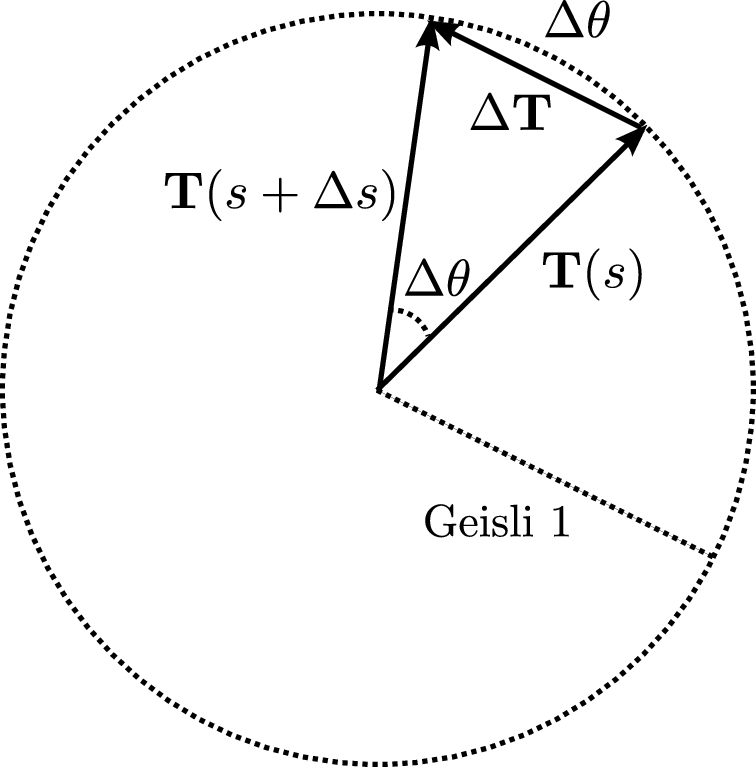
\includegraphics[width=0.400\linewidth]{krappi.png}\hfill}


\section{Hjúfurplan}
\label{Kafli1:hjufurplan}
\index{hjúfur-!plan}\index{hjúfur-!hringur}

\subsection{Skilgreining}
\label{Kafli1:index-17}\label{Kafli1:id17}
Látum \(\cal C\) vera feril í plani eða rúmi og
\(\mbox{${\bf r}$}\) stikun á \(\cal C\) með bogalengd.

\textit{Hjúfurplanið} við ferilinn í punkti
\(\mbox{${\bf r}$}(s)\) er planið sem spannað er af vigrunum
\(\mbox{${\bf T}$}(s)\) og \(\mbox{${\bf N}$}(s)\) og liggur um
punktinn \(\mbox{${\bf r}$}(s)\).

\textit{Hjúfurhringur} við ferilinn í punkti
\(\mbox{${\bf r}$}(s)\) er hringur sem liggur í hjúfurplaninu, fer í
gegnum punktinn \(\mbox{${\bf r}$}(s)\), hefur geisla
\(\rho(s)\) og hefur miðju í punktinum
\(\mbox{${\bf r}$}(s)+\rho(s)\mbox{${\bf N}$}(s)\).


\section{Tvíþverill}
\label{Kafli1:tviverill}
\index{tvíþverill}\index{Frenet ramminn}

\subsection{Skilgreining}
\label{Kafli1:id18}\label{Kafli1:index-18}
Látum \(\cal C\) vera feril í plani eða rúmi og
\(\mbox{${\bf r}$}\) stikun á \(\cal C\) með bogalengd. Vigurinn
\begin{gather}
\begin{split}\displaystyle \mbox{${\bf B}$}(s)=\mbox{${\bf T}$}(s)\times \mbox{${\bf N}$}(s)\end{split}\notag
\end{gather}
kallast \textit{tvíþverill} við ferilinn í
\(\mbox{${\bf r}$}(s)\).

\(\{\mbox{${\bf T}$}(s),\mbox{${\bf N}$}(s),\mbox{${\bf B}$}(s)\}\)
er þverstaðlaður grunnur og kallast \textbf{Frenet ramminn}.


\section{Vindingur}
\label{Kafli1:vindingur}
\index{vindingur}

\subsection{Setning og skilgreining}
\label{Kafli1:index-19}\label{Kafli1:setning-og-skilgreining}
Látum \(\cal C\) vera feril í plani eða rúmi og
\(\mbox{${\bf r}$}\) stikun á \(\cal C\) með bogalengd. Vigurinn
\(\mbox{${\bf B}$}'(s)\) er samsíða vigrinum
\(\mbox{${\bf N}$}(s)\), þ.e.a.s. \(\mbox{${\bf B}$}'(s)\) er
margfeldi af \(\mbox{${\bf N}$}(s)\). Talan \(\tau(s)\) þannig
að
\begin{gather}
\begin{split}\displaystyle \mbox{${\bf B}$}'(s)=-\tau(s)\mbox{${\bf N}$}(s)\end{split}\notag
\end{gather}
kallast \textit{vindingur} ferilsins í punktinum \(\mbox{${\bf r}$}(s)\).


\section{Frenet-Serret jöfnurnar}
\label{Kafli1:frenet-serret-jofnurnar}
\index{Frenet-Serret}

\subsection{Jöfnur}
\label{Kafli1:jofnur}\label{Kafli1:index-20}
Látum \(\cal C\) vera feril í plani eða rúmi og
\(\mbox{${\bf r}$}\) stikun á \(\cal C\) með bogalengd. Þá
gildir
\begin{gather}
\begin{split}\displaystyle\end{split}\notag\\\begin{split}\begin{aligned}
\mbox{${\bf T}$}'(s)&=\kappa\mbox{${\bf N}$}\\
\mbox{${\bf N}$}'(s)&=-\kappa\mbox{${\bf T}$}+\tau\mbox{${\bf B}$}\\
\mbox{${\bf B}$}'(s)&=-\tau\mbox{${\bf N}$}.\end{aligned}\end{split}\notag
\end{gather}

\subsection{Setning}
\label{Kafli1:id19}
Látum \(\cal C\) vera feril í plani eða rúmi. Gerum ráð fyrir að
\(\mbox{${\bf r}$}\) sé þjáll stikaferill sem stikar \(\cal C\).
Ritum \(\mbox{${\bf v}$}=\mbox{${\bf r}$}'(t)\) og
\(\mbox{${\bf a}$}=\mbox{${\bf r}$}''(t)\). Þá gildir í punktinum
\(\mbox{${\bf r}$}(t)\) að
\begin{gather}
\begin{split}\displaystyle\end{split}\notag\\\begin{split}\mbox{${\bf T}$}=\frac{\mbox{${\bf v}$}}{|\mbox{${\bf v}$}|},\qquad
\mbox{${\bf B}$}=\frac{\mbox{${\bf v}$}\times\mbox{${\bf a}$}}{|\mbox{${\bf v}$}\times\mbox{${\bf a}$}|},\qquad
\mbox{${\bf N}$}=\mbox{${\bf B}$}\times\mbox{${\bf T}$},\end{split}\notag
\end{gather}
einnig er
\begin{gather}
\begin{split}\displaystyle\end{split}\notag\\\begin{split}\kappa=\frac{|\mbox{${\bf v}$}\times\mbox{${\bf a}$}|}{|\mbox{${\bf v}$}|^3},\qquad\qquad
\tau=\frac{(\mbox{${\bf v}$}\times\mbox{${\bf a}$})\cdot \frac{d}{dt}\mbox{${\bf a}$}}{|\mbox{${\bf v}$}\times\mbox{${\bf a}$}|^2}.\end{split}\notag
\end{gather}

\chapter{Hlutafleiður}
\label{Kafli2::doc}\label{Kafli2:hlutafleiur}
\emph{“If you need help bark like a dog.'' - Gendry. ``That's stupid. If I need help I'll shout help.'' - Arya”}

- George R.R. Martin, A Clash of Kings


\section{Graf falls}
\label{Kafli2:graf-falls}
\index{graf falls}

\subsection{Skilgreining}
\label{Kafli2:skilgreining}\label{Kafli2:index-0}
Látum \(f:{\mathbb  R}^2\rightarrow {\mathbb  R}\) vera fall. \emph{Graf}
fallsins er skilgreint sem mengið
\begin{gather}
\begin{split}\displaystyle \{(x,y,f(x,y))\mid (x,y)\in{\mathbb  R}^2\}\subseteq {\mathbb  R}^3.\end{split}\notag
\end{gather}
Ef \(f:{\mathbb  R}^3\rightarrow {\mathbb  R}\) er fall, þá er
\emph{graf} fallsins skilgreint sem mengið
\begin{gather}
\begin{split}\displaystyle \{(x,y,z,f(x,y,z))\mid (x,y,z)\in{\mathbb  R}^3\}\subseteq {\mathbb  R}^4.\end{split}\notag
\end{gather}
{\hfill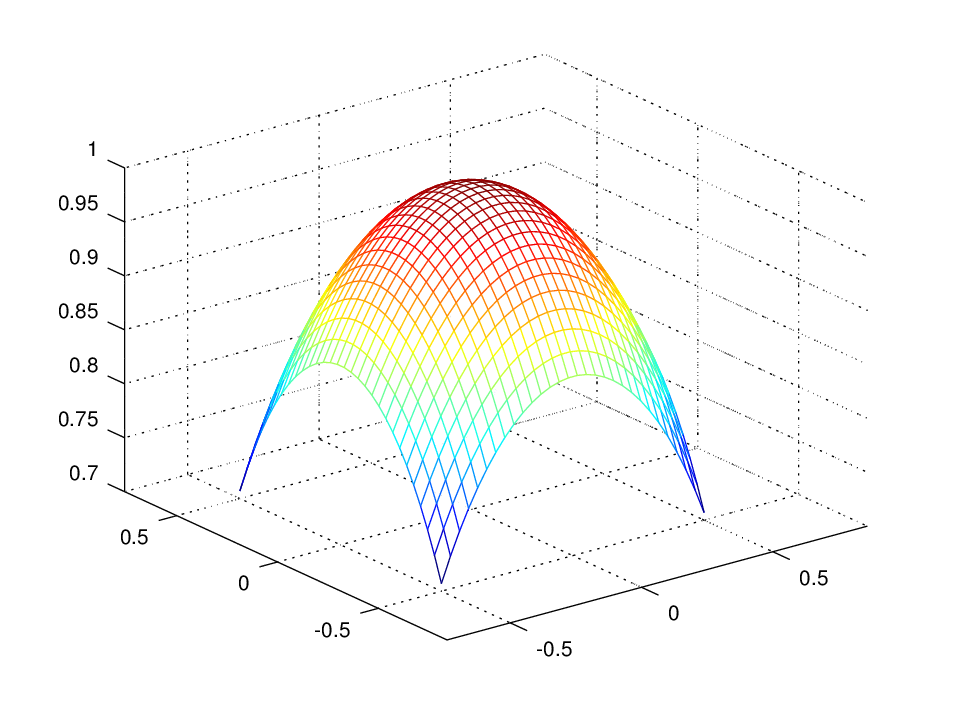
\includegraphics[width=0.600\linewidth]{surface.png}\hfill}

\emph{Graf fallsins} \(f(x,y) = \sqrt{1-x^2-y^2}\), \(-0.5\leq x,y\leq 0.5\).


\section{Jafnhæðarlínur}
\label{Kafli2:jafnhaearlinur}
\index{jafnhæðar-!lína}\index{jafnhæðar-!ferill}\index{jafnhæðar-!flötur}

\subsection{Skilgreining}
\label{Kafli2:id1}\label{Kafli2:index-1}
Látum \(f:{\mathbb  R}^2\rightarrow {\mathbb  R}\) vera fall. Ef
\(c\) er fasti þá er mengið
\begin{gather}
\begin{split}\displaystyle \{(x,y)\mid f(x,y)=c\}\subseteq {\mathbb  R}^2\end{split}\notag
\end{gather}
kallað \textit{jafnhæðarlína} eða \textit{jafnhæðarferill} fallsins
\(f\) fyrir fastann \(c\).

Látum \(f:{\mathbb  R}^3\rightarrow {\mathbb  R}\) vera fall. Ef
\(c\) er fasti þá er mengið
\begin{gather}
\begin{split}\displaystyle \{(x,y,z)\mid f(x,y,z)=c\}\end{split}\notag
\end{gather}
kallað \textit{jafnhæðarflötur} fallsins \(f\) fyrir
fastann \(c\).

{\hfill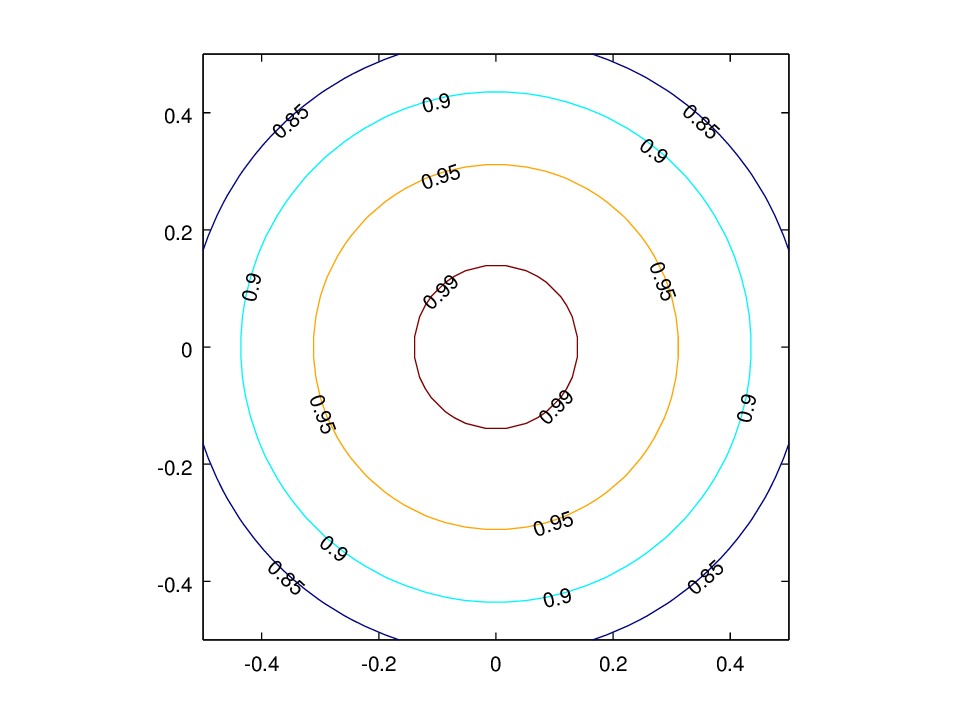
\includegraphics[width=0.600\linewidth]{contour.png}\hfill}

\emph{Nokkrar jafnæðarlínur fallsins} \(f(x,y) = \sqrt{1-x^2-y^2}\), \(-0.5\leq x,y\leq 0.5\).


\section{Fjarlægð milli punkta}
\label{Kafli2:fjarlaeg-milli-punkta}
\index{fjarlægð}

\subsection{Skilgreining}
\label{Kafli2:id2}\label{Kafli2:index-2}
\emph{Fjarlægðin} milli tveggja punkta
\(\mbox{${\bf x}$}=(x_1,x_2, \ldots,x_n)\) og
\(\mbox{${\bf y}$}=(y_1,y_2, \ldots,y_n)\) í
\(\mbox{${\bf R}^n$}\) er skilgreind sem talan
\begin{gather}
\begin{split}\displaystyle |\mbox{${\bf x}$}-\mbox{${\bf y}$}|=\sqrt{(x_1-y_1)^2+(x_2-y_2)^2+\cdots+(x_n-y_n)^2}.\end{split}\notag
\end{gather}

\section{Opnar kúlur}
\label{Kafli2:opnar-kulur}
\index{opin kúla}

\subsection{Skilgreining}
\label{Kafli2:index-3}\label{Kafli2:id3}
Látum \(P=(p_1,p_2,\ldots,p_n)\) vera punkt í
\(\mbox{${\bf R}^n$}\). Skilgreinum \emph{opnu kúluna} með miðju í
\(P\) og geisla \(r\) sem mengið
\begin{gather}
\begin{split}\displaystyle B_r(P)=\{Q\in\mbox{${\bf R}^n$}\mid |Q-P|<r\}.\end{split}\notag
\end{gather}
Í \({\mathbb  R}^2\) er eðlilegra að tala um \emph{opna skífu} eða \emph{opinn
disk} í stað opinnar kúlu og í \({\mathbb  R}\) þá er talað um opin
bil.


\section{Opin mengi}
\label{Kafli2:opin-mengi}
\index{opið mengi}\index{lokað mengi}\index{fyllimengi}

\subsection{Skilgreining}
\label{Kafli2:index-4}\label{Kafli2:id4}
Látum \(U\) vera hlutmengi í \(\mbox{${\bf R}^n$}\).

Sagt er að \(U\) sé \textit{opið mengi} ef um sérhvern punkt \(P\) í
\(U\) gildir að til er tala \(r>0\) þannig að
\(B_r(P)\subseteq U\).

Mengið \(U\) er sagt \textit{lokað} ef \textit{fyllimengið} er opið. (\emph{Fyllimengi}
\(U\) er skilgreint sem mengið
\(\mbox{${\bf R}^n$}\setminus U=\{Q\in \mbox{${\bf R}^n$}\mid Q\mbox{$\;\not\in\;$}U\}\).)


\section{Jaðarpunktur}
\label{Kafli2:jaarpunktur}
\index{jaðarpunktur}

\subsection{Skilgreining}
\label{Kafli2:index-5}\label{Kafli2:id5}
Látum \(U\) vera mengi í \(\mbox{${\bf R}^n$}\). Punktur
\(P\) í \(\mbox{${\bf R}^n$}\) er sagður \textit{jaðarpunktur}
\(U\) ef sérhver opin kúla \(B_r(P)\) með \(r>0\) inniheldur
bæði punkt úr \(U\) og punkt úr
\(\mbox{${\bf R}^n$}\setminus U\). (Athugið að bæði er mögulegt að
jaðarpunktur \(U\) sé í \(U\) og að hann sé ekki í \(U\).)


\section{Skilgreiningarmengi}
\label{Kafli2:skilgreiningarmengi}
\index{skilgreiningarmengi}

\subsection{Skilgreining}
\label{Kafli2:id6}\label{Kafli2:index-6}
Fyrir fall \(f(x_1,x_2,\ldots,x_n)\) þá táknar \({\cal D}(f)\)
\textit{skilgreiningarmengi} fallsins \(f\). Ef fallið er gefið með formúlu
og ekkert sagt um \({\cal D}(f)\) þá lítum við svo á að
\({\cal D}(f)\) sé mengi allra punkta í \(\mbox{${\bf R}^n$}\)
þannig að formúlan gefi vel skilgreinda tölu.

\index{markgildi}\index{stefna á}

\section{Markgildi}
\label{Kafli2:index-7}\label{Kafli2:markgildi}

\subsection{Skilgreining}
\label{Kafli2:id7}
Látum \(f(x_1,x_2,\ldots,x_n)\) vera fall af \(n\) breytistærðum
með skilgreiningarmengi \({\cal D}(f)\subseteq \mbox{${\bf R}^n$}\).
Látum \(P=(p_1,p_2,\ldots,p_n)\) vera punkt í
\(\mbox{${\bf R}^n$}\) þannig að sérhver opin kúla um \(P\)
inniheldur meira en einn punkt úr \({\cal D}(f)\).

Segjum að \(f(x_1,x_2,\ldots,x_n)\) \textit{stefni á} tölu \(L\) þegar
\((x_1,x_2,\ldots,x_n)\) stefnir á \((p_1,p_2,\ldots,p_n)\) ef
eftirfarandi gildir:

Fyrir sérhverja tölu \(\epsilon>0\) er til tala \(\delta>0\)
þannig að ef \((x_1,x_2,\ldots,x_n)\in{\cal D}(f)\) og
\begin{gather}
\begin{split}\displaystyle\end{split}\notag\\\begin{split}|(x_1,x_2,\ldots,x_n)-(p_1,p_2,\ldots,p_n)|<\delta\end{split}\notag
\end{gather}
þá er
\begin{gather}
\begin{split}\displaystyle
|f(x_1,x_2,\ldots,x_n)-L|<\epsilon.\end{split}\notag
\end{gather}

\subsection{Ritháttur}
\label{Kafli2:rithattur}
Ef \(f(x_1,x_2,\ldots,x_n)\) stefnir á tölu \(L\) þegar
\((x_1,x_2,\ldots,x_n)\) stefnir á \((p_1,p_2,\ldots,p_n)\) þá
er ritað
\begin{gather}
\begin{split}\displaystyle\end{split}\notag\\\begin{split}\lim_{(x_1,x_2,\ldots,x_n)\rightarrow (p_1,p_2,\ldots,p_n)}
f(x_1,x_2,\ldots,x_n)=L.\end{split}\notag
\end{gather}
og \(L\) kallast \textit{markgildi} fallsins \(f\) í punktinum \((x_1,x_2,\ldots,x_n)\).


\subsection{Skilgreining (Skilgreining 2.8.1 sett fram fyrir föll af tveimur breytum.)}
\label{Kafli2:skilgreining-skilgreining-2-8-1-sett-fram-fyrir-foll-af-tveimur-breytum}
Látum \(f(x,y)\) vera fall skilgreint á mengi
\({\cal D}(f)\subseteq {\mathbb  R}^2\). Látum \((a,b)\) vera
punkt í \({\mathbb  R}^2\) þannig að sérhver opin skífa um
\((a,b)\) inniheldur meira en einn punkt úr \({\cal D}(f)\).

Segjum að \(f(x,y)\) stefni á tölu \(L\) þegar \((x,y)\)
stefnir á \((a,b)\) ef eftirfarandi gildir:

Fyrir sérhverja tölu \(\epsilon>0\) er til tala \(\delta>0\)
þannig að ef \((x,y)\in{\cal D}(f)\) og
\begin{gather}
\begin{split}\displaystyle\end{split}\notag\\\begin{split}\delta > |(x,y)-(a,b)| = \sqrt{(x-a)^2+(y-b)^2}\end{split}\notag
\end{gather}
þá er
\begin{gather}
\begin{split}\displaystyle
|f(x,y)-L|<\epsilon.\end{split}\notag
\end{gather}

\section{Reglur um markgildi}
\label{Kafli2:reglur-um-markgildi}

\subsection{Setning}
\label{Kafli2:setning}
Látum \(f\) og \(g\) vera föll af tveimur breytum. Gerum ráð
fyrir að
\begin{gather}
\begin{split}\displaystyle\end{split}\notag\\\begin{split}\lim_{(x,y)\rightarrow (a,b)}f(x,y)=L\quad\mbox{og}\quad
\lim_{(x,y)\rightarrow (a,b)}g(x,y)=M,\end{split}\notag
\end{gather}
og að sérhver \textit{grennd} um \((a,b)\) innihaldi fleiri en einn punkt þar
sem bæði föllin \(f\) og \(g\) eru skilgreind. Þá gildir

\textbf{(a)} \(\lim_{(x,y)\rightarrow (a,b)}(f(x,y)\pm g(x,y))=L\pm M\).

\textbf{(b)} \(\lim_{(x,y)\rightarrow (a,b)}f(x,y) g(x,y)=LM\).

\textbf{(c)} \(\lim_{(x,y)\rightarrow (a,b)}\frac{f(x,y)}{g(x,y)}=
\frac{L}{M}\), svo framarlega sem \(M\neq 0\).

\textbf{(d)} \(\lim_{(x,y)\rightarrow (a,b)}F(f(x,y))=F(L)\) ef \(F\)
er fall af einni breytistærð sem er samfellt í punktinum \(L\).

\index{samfelldni}

\section{Samfelldni}
\label{Kafli2:index-8}\label{Kafli2:samfelldni}

\subsection{Skilgreining}
\label{Kafli2:id8}
Látum \(f\) vera fall af \(n\) breytistærðum skilgreint á mengi
\({\cal D}(f)\) í \(\mbox{${\bf R}^n$}\). Fallið \(f\) er
sagt \emph{samfellt í punkti} \((p_1,p_2,\ldots,p_n)\) í
\({\cal D}(f)\) ef
\begin{gather}
\begin{split}\displaystyle\end{split}\notag\\\begin{split}\lim_{(x_1,x_2,\ldots,x_n)\rightarrow (p_1,p_2,\ldots,p_n)}
f(x_1,x_2,\ldots,x_n)=f(p_1,p_2,\ldots,p_n).\end{split}\notag
\end{gather}
Sagt er að fallið sé \textit{samfellt} ef það er samfellt í öllum punktum
skilgreiningarmengis síns.


\section{Hlutafleiður}
\label{Kafli2:id9}
\index{hlutafleiða}

\subsection{Skilgreining}
\label{Kafli2:id10}\label{Kafli2:index-9}
Látum \(f(x,y)\) vera fall af tveimur breytum \(x\) og \(y\)
sem er skilgreint á opinni skífu með miðju í punktinum \((a,b)\).

Skilgreinum \textit{hlutafleiðu} m.t.t. \(x\) í \((a,b)\) með
\begin{gather}
\begin{split}\displaystyle f_1(a,b)=\lim_{h\rightarrow 0}\frac{f(a+h,b)-f(a,b)}{h}\end{split}\notag
\end{gather}
og \textit{hlutafleiðu} m.t.t. \(y\) í \((a,b)\) með
\begin{gather}
\begin{split}\displaystyle f_2(a,b)=\lim_{k\rightarrow 0}\frac{f(a,b+k)-f(a,b)}{k}\end{split}\notag
\end{gather}
ef markgildin eru til.

{\hfill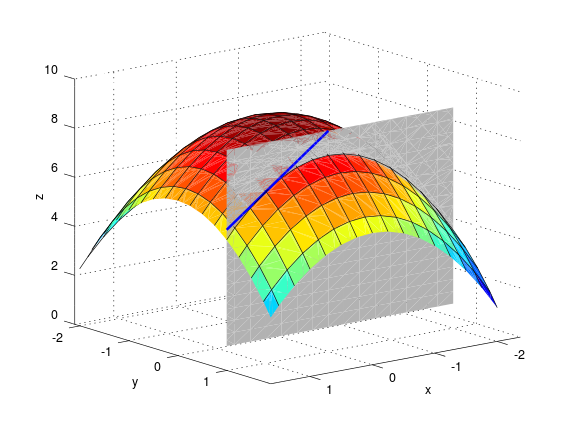
\includegraphics[width=0.600\linewidth]{xpart.png}\hfill}

\emph{Hlutafleiða m.t.t.} \(x\) \emph{fyrir} \(y=1\).

{\hfill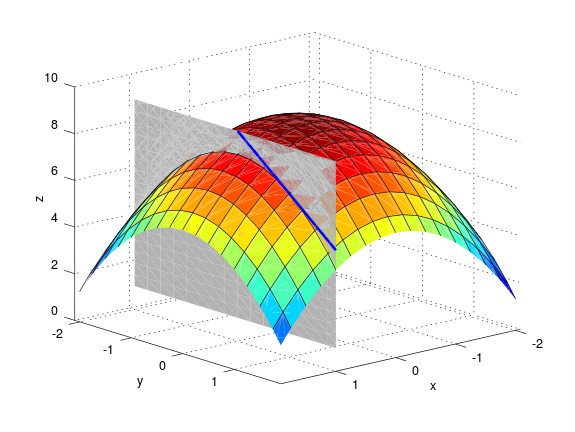
\includegraphics[width=0.600\linewidth]{ypart.png}\hfill}

\emph{Hlutafleiða m.t.t.} \(y\) \emph{fyrir} \(x=1\).


\subsection{Skilgreining}
\label{Kafli2:id11}
Látum \(f(x,y,z)\) vera fall af þremur breytum \(x\), \(y\)
og \(z\) sem er skilgreint á opinni kúlu með miðju í punktinum
\((a, b,c)\).

Skilgreinum \emph{hlutafleiðu m.t.t.} \(x\) í \((a,b,c)\) með
\begin{gather}
\begin{split}\displaystyle f_1(a,b,c)=\lim_{h\rightarrow 0}\frac{f(a+h,b,c)-f(a,b,c)}{h},\end{split}\notag
\end{gather}
\emph{hlutafleiðu m.t.t.} \(y\) í \((a,b,c)\) með
\begin{gather}
\begin{split}\displaystyle f_2(a,b,c)=\lim_{k\rightarrow 0}\frac{f(a,b+k,c)-f(a,b,c)}{k}\end{split}\notag
\end{gather}
og \emph{hlutafleiðu m.t.t.} \(z\) í \((a,b,c)\) með
\begin{gather}
\begin{split}\displaystyle f_3(a,b,c)=\lim_{\ell\rightarrow 0}\frac{f(a,b,c+\ell)-f(a,b,c)}{\ell}\end{split}\notag
\end{gather}
ef markgildin eru til.


\subsection{Skilgreining}
\label{Kafli2:id12}
Látum \(f\) vera fall af \(n\) breytum
\(x_1,x_2,\ldots,x_n\) sem er skilgreint á opinni kúlu um punktinn
\(\mathbf{a}=(a_1, a_2, \ldots, a_n).\)

Hlutafleiða \(f\) með tilliti til breytunnar \(x_k\) í punktinum
\(\mathbf{a}\) er skilgreind sem markgildið
\begin{gather}
\begin{split}\displaystyle f_k(\mathbf{a})=\lim_{h\rightarrow 0}\frac{f(\mathbf{a}+h\mbox{${\bf e}$}_k)-f(\mathbf{a})}{h}\end{split}\notag
\end{gather}
ef markgildið er til. (Hér stendur \(\mbox{${\bf e}$}_k\) fyrir
vigurinn sem er með 0 í öllum hnitum nema því \(k\)-ta þar sem er
1.)


\subsection{Ritháttur}
\label{Kafli2:id13}
Ritum \(z=f(x,y)\).  Ýmis konar ritháttur er fyrir hlutafleiður, m.a.
\begin{gather}
\begin{split}\displaystyle\end{split}\notag\\\begin{split}\begin{aligned}
f_1(x,y)&=\frac{\partial z}{\partial x}=  \frac{\partial }{\partial x}f(x,y)
=D_1f(x,y)=f_x(x,y)=D_xf(x,y)=\partial_xf(x,y) \\
f_2(x,y)&=\frac{\partial z}{\partial y}=  \frac{\partial }{\partial y}f(x,y)
=D_2f(x,y)=f_y(x,y)=D_yf(x,y)=\partial_yf(x,y). \end{aligned}\end{split}\notag
\end{gather}
Þegar við viljum tákna gildið á hlutafleiðu \(f\) í ákveðnum punkti
\((x,y)=(a,b)\) þá eru líka ýmsir möguleikar, til dæmis
\begin{gather}
\begin{split}\displaystyle\end{split}\notag\\\begin{split}\begin{aligned}
\frac{\partial z}{\partial x}\bigg|_{(a,b)}&=
\left(\frac{\partial }{\partial x}f(x,y)\right)\bigg|_{(a,b)}
=f_1(a,b)=D_1f(a,b) \\
\frac{\partial z}{\partial y}\bigg|_{(a,b)}&=
\left(\frac{\partial }{\partial y}f(x,y)\right)\bigg|_{(a,b)}
=f_2(a,b)=D_2f(a,b). \end {aligned}\end{split}\notag
\end{gather}
\begin{notice}{warning}{Aðvörun:}
Strangt til tekið merkir rithátturinn \(\frac{\partial}{\partial x} f(a,b)\) að við stingum fyrst
inn tölunum \(a\) og \(b\) og diffrum síðan með tilliti til \(x\). En þar sem \(f(a,b)\) er
óháð \(x\) er útkoman 0.
\end{notice}


\section{Snertiplan}
\label{Kafli2:snertiplan}
Látum \(f(x,y)\) vera fall af tveimur breytistærðum þannig að
hlutafleiðurnar \(f_1(a,b)\) og \(f_2(a,b)\) séu skilgreindar.

{\hfill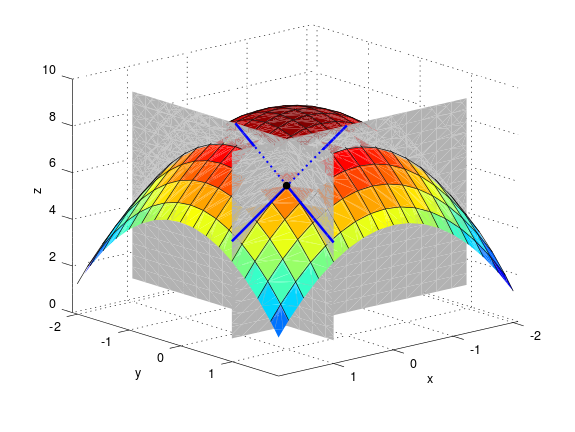
\includegraphics[width=0.600\linewidth]{bothpart.png}\hfill}

Í punktinum \((a,b,f(a,b))\) er

\(\mbox{${\bf T}$}_1 = \mbox{${\bf i}$}+ f_1(a,b)\mbox{${\bf k}$}\qquad\)
\textit{snertivigur} við ferilinn \(f(x,b) = z\) og

\(\mbox{${\bf T}$}_2 = \mbox{${\bf j}$}+ f_2(a,b)\mbox{${\bf k}$}\qquad\)
\textit{snertivigur} við ferilinn \(f(a,y) = z\).

Táknum með \(S\) planið sem hefur stikunina
\begin{gather}
\begin{split}\displaystyle (a,b,f(a,b))+s\mbox{${\bf T}$}_1+t\mbox{${\bf T}$}_2, \quad -\infty < s,t < \infty.\end{split}\notag
\end{gather}
Vigurinn
\begin{gather}
\begin{split}\displaystyle \mbox{${\bf n}$}=\mbox{${\bf T}$}_2\times \mbox{${\bf T}$}_1=f_1(a,b)\mbox{${\bf i}$}+f_2(a,b)\mbox{${\bf j}$}-\mbox{${\bf k}$}\end{split}\notag
\end{gather}
er þvervigur á \(S\) og jafna plansins \(S\) er
\begin{gather}
\begin{split}\displaystyle z=f(a,b)+f_1(a,b)(x-a)+f_2(a,b)(y-b).\end{split}\notag
\end{gather}
\textit{Þverlína} á \(S\) hefur stikun
\begin{gather}
\begin{split}\displaystyle (a,b,f(a,b)) + u \mbox{${\bf n}$}, \quad -\infty < u < \infty.\end{split}\notag
\end{gather}
Ef \(f(x,y)\) er ’nógu nálægt’ (skilgreint nánar síðar) planinu
\(S\) þegar \((x,y)\) er nálægt punktinum \((a,b)\) þá
kallast \(S\) \textit{snertiplan} við grafið \(z=f(x,y)\) í punktinum
\((a,b,f(a,b))\).


\section{Hlutafleiður af hærra stigi}
\label{Kafli2:hlutafleiur-af-haerra-stigi}
\index{hlutafleiða!annars stigs}\index{hlutafleiða!hrein}\index{hlutafleiða!blönduð}

\subsection{Skilgreining}
\label{Kafli2:id14}\label{Kafli2:index-10}
Ritum \(z=f(x,y)\). \emph{Annars stigs hlutafleiður} \(f\) eru
skilgreindar með formúlunum
\begin{gather}
\begin{split}\displaystyle\end{split}\notag\\\begin{split}\frac{\partial^2 z}{\partial x^2}=
\frac{\partial}{\partial x} \frac{\partial z}{\partial x}
=f_{11}(x,y)=f_{xx}(x,y),\end{split}\notag
\end{gather}\begin{gather}
\begin{split}\displaystyle\end{split}\notag\\\begin{split}\frac{\partial^2 z}{\partial y^2}=
\frac{\partial}{\partial y} \frac{\partial z}{\partial y}
=f_{22}(x,y)=f_{yy}(x,y),\end{split}\notag
\end{gather}\begin{gather}
\begin{split}\displaystyle\end{split}\notag\\\begin{split}\frac{\partial^2 z}{\partial x\partial y}=
\frac{\partial}{\partial x} \frac{\partial z}{\partial y}
=f_{21}(x,y)=f_{yx}(x,y),\end{split}\notag
\end{gather}\begin{gather}
\begin{split}\displaystyle\end{split}\notag\\\begin{split}\frac{\partial^2 z}{\partial y\partial x}=
\frac{\partial}{\partial y} \frac{\partial z}{\partial x}
=f_{12}(x,y)=f_{xy}(x,y).\end{split}\notag
\end{gather}
Hlutafleiðurnar \(f_{11}(x,y)\) og \(f_{22}(x,y)\) kallast
hreinar hlutafleiður og \(f_{12}(x,y)\) og \(f_{21}(x,y)\)
kallast blandaðar hlutafleiður.


\subsection{Setning}
\label{Kafli2:id15}
Látum \(f(x,y)\) vera fall sem er skilgreint á opinni skífu
\(D\) með miðju í \(P=(a,b)\) . Gerum ráð fyrir að
hlutafleiðurnar \(f_1(x,y)\), \(f_2(x,y)\), \(f_{12}(x,y)\)
og \(f_{21}(x,y)\) séu allar skilgreindar á \(D\) og að þær séu
allar samfelldar á \(D\). Þá gildir að
\begin{gather}
\begin{split}\displaystyle f_{12}(a,b)=f_{21}(a,b).\end{split}\notag
\end{gather}

\subsection{Hugmynd að skilgreiningu}
\label{Kafli2:hugmynd-a-skilgreiningu}
Skilgreiningu 5.6 má útvíkka á augljósan hátt til að skilgreina 2. stigs
hlutafleiður fyrir föll af fleiri en tveimur breytum. Einnig er augljóst
hvernig má skilgreina hlutafleiður af hærri stigum en 2, til dæmis ef
\(w=f(x,y,z)\) þá
\begin{gather}
\begin{split}\displaystyle\end{split}\notag\\\begin{split}\frac{\partial^3 w}{\partial x\partial y^2} \quad\quad\mbox{(diffra
    fyrst tvisvar m.t.t. }y\mbox{, svo einu sinni m.t.t. } x\mbox{)}\end{split}\notag
\end{gather}
og
\begin{gather}
\begin{split}\displaystyle\end{split}\notag\\\begin{split}\frac{\partial^3 w}{\partial y\partial z\partial y} \quad\quad\mbox{(diffra
    fyrst m.t.t. } y\mbox{, svo m.t.t. } z
\mbox{ og að lokum m.t.t. }y\mbox{)}.\end{split}\notag
\end{gather}

\subsection{Setning (Almenn útgáfa af Setningu 2.13.2)}
\label{Kafli2:setning-almenn-utgafa-af-setningu-2-13-2}
Látum \(f\) vera fall \(n\) breytistærðum sem er skilgreint á
opinni kúlu með miðju í \(P=(x_1, x_2,\ldots, x_n)\).

Skoðum tvær hlutafleiður \(f\) í punktum \(P\) þar sem er
diffrað með tilliti til sömu breytistærða og jafn oft með tilliti til
hverrar breytistærðar. Ef þessar hlutafleiður eru samfelldar í punktinum
\(P\) og allar hlutafleiður af lægra stigi eru skilgreindar á
\(D\) og samfelldar á \(D\) þá eru hlutafleiðurnar sem við erum
að skoða jafnar í \(P\).


\subsection{Dæmi:}
\label{Kafli2:daemi}
Ef \(w = f(x,y,z)\) er fall af þremur breytistærðum þá er t.d.
\begin{gather}
\begin{split}\displaystyle \frac{\partial^4 w}{\partial x^2\partial y \partial z} = \frac{\partial^4 w}{\partial x \partial y \partial x \partial z}\end{split}\notag
\end{gather}
ef skilyrðin í setningunni eru uppfyllt.

\index{keðjuregla}

\section{\textit{Keðjuregla}}
\label{Kafli2:id16}\label{Kafli2:index-11}
\index{keðjuregla!í einni breytistærð}

\subsection{Setning (Keðjureglan í einni breytistærð.)}
\label{Kafli2:index-12}\label{Kafli2:setning-kejureglan-i-einni-breytistaer}
Gerum ráð fyrir að fallið \(f(u)\) sé diffranlegt í punktinum
\(u=g(x)\) og að fallið \(g(x)\) sé diffranlegt í punktinum
\(x\). Þá er fallið \((f\circ g)(x)=f(g(x))\) diffranlegt í
\(x\) og
\begin{gather}
\begin{split}\displaystyle (f\circ g)'(x)=f'(g(x))g'(x).\end{split}\notag
\end{gather}

\subsection{Setning}
\label{Kafli2:id17}
Látum \(f(x,y)\) vera fall þar sem \(x=x(t)\) og \(y=y(t)\)
eru föll af breytu \(t\). Gerum ráð fyrir að á opinni skífu um
punktinum \((x(t),y(t))\) séu báðar fyrsta stigs hlutafleiður
\(f\) skilgreindar og samfelldar. Gerum enn fremur ráð fyrir að
föllin \(x(t)\) og \(y(t)\) séu bæði diffranleg í punktinum
\(t\). Þá er fallið
\begin{gather}
\begin{split}\displaystyle g(t)=f(x(t),y(t))\end{split}\notag
\end{gather}
diffranlegt í \(t\) og
\begin{gather}
\begin{split}\displaystyle g'(t)=f_1(x(t),y(t))x'(t)+f_2(x(t),y(t))y'(t).\end{split}\notag
\end{gather}

\subsection{Ritháttur}
\label{Kafli2:id18}
Ritum \(z=f(x,y)\) þar sem \(x=x(t)\) og \(y=y(t)\) eru föll
af breytu \(t\). Þá er
\begin{gather}
\begin{split}\displaystyle\end{split}\notag\\\begin{split}\frac{dz}{dt}=\frac{\partial z}{\partial x}\frac{dx}{dt}
+\frac{\partial z}{\partial y}\frac{dy}{dt}.\end{split}\notag
\end{gather}
{\hfill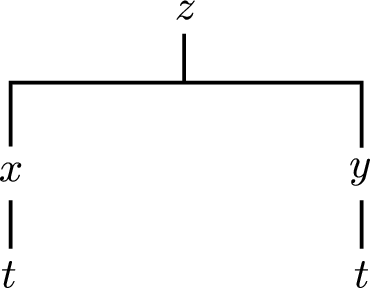
\includegraphics[width=0.270\linewidth]{chain1.png}\hfill}


\subsection{Setning}
\label{Kafli2:id19}
Látum \(f(x,y)\) vera fall af breytistærðum \(x\) og \(y\)
sem aftur eru föll af breytum \(s\) og \(t\), það er að segja
\(x=x(s,t)\) og \(y=y(s,t)\). Ritum svo
\begin{gather}
\begin{split}\displaystyle g(s,t)=f(x(s,t),y(s,t)).\end{split}\notag
\end{gather}
Þá gildir (að gefnum sambærilegum skilyrðum og í 2.14.2) að
\begin{gather}
\begin{split}\displaystyle g_1(s,t)=f_1(x(s,t),y(s,t))x_1(s,t)+f_2(x(s,t),y(s,t))y_1(s,t),\end{split}\notag\\\begin{split}og\end{split}\notag
\end{gather}\begin{gather}
\begin{split}\displaystyle g_2(s,t)=f_1(x(s,t),y(s,t))x_2(s,t)+f_2(x(s,t),y(s,t))y_2(s,t).\end{split}\notag
\end{gather}

\subsection{Ritháttur}
\label{Kafli2:id20}
Ritum \(z=f(x,y)\) þar sem \(x=x(s,t)\) og \(y=y(s,t)\) eru
föll af breytum \(s\) og \(t\). Þá er
\begin{gather}
\begin{split}\displaystyle\end{split}\notag\\\begin{split}\frac{\partial z}{\partial s}=
\frac{\partial z}{\partial x}\frac{\partial x}{\partial s}
+\frac{\partial z}{\partial y}\frac{\partial y}{\partial s}, \quad \text{og}\quad \frac{\partial z}{\partial t}=
\frac{\partial z}{\partial x}\frac{\partial x}{\partial t}
+\frac{\partial z}{\partial y}\frac{\partial y}{\partial t}.\end{split}\notag
\end{gather}\begin{figure}[htbp]
\centering

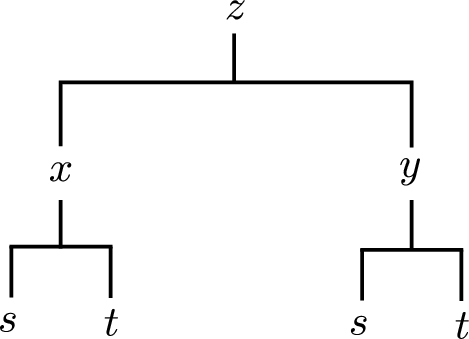
\includegraphics[width=0.300\linewidth]{chain2.png}
\end{figure}


\subsection{Ritháttur}
\label{Kafli2:id21}
Ritum \(z=f(x,y)\) þar sem \(x=x(s,t)\) og \(y=y(s,t)\) eru
föll af breytum \(s\) og \(t\). Þá er
\begin{gather}
\begin{split}\displaystyle\end{split}\notag\\\begin{split}\begin{bmatrix}\frac{\partial z}{\partial s}
& \frac{\partial z}{\partial t}\end{bmatrix}
=\begin{bmatrix}\frac{\partial z}{\partial x}
& \frac{\partial z}{\partial y}\end{bmatrix}
\begin{bmatrix}\frac{\partial x}{\partial s}
& \frac{\partial x}{\partial t}\\
\frac{\partial y}{\partial s}
& \frac{\partial y}{\partial t}
\end{bmatrix}\end{split}\notag
\end{gather}

\subsection{Setning}
\label{Kafli2:id22}
Látum \(u\) vera fall af \(n\) breytum
\(x_1, x_2, \ldots, x_n\) þannig að hvert \(x_i\) má rita sem
fall af \(m\) breytum \(t_1, t_2, \ldots, t_m\). Gerum ráð fyrir
að allar hlutafleiðurnar \(\frac{\partial u}{\partial x_i}\) og
\(\frac{\partial x_i}{\partial t_j}\) séu til og samfelldar. Þegar
\(u\) er skoðað sem fall af breytunum \(t_1, t_2, \ldots, t_m\)
fæst að
\begin{gather}
\begin{split}\displaystyle\end{split}\notag\\\begin{split}\frac{\partial u}{\partial t_j}=
\frac{\partial u}{\partial x_1}\frac{\partial x_1}{\partial t_j}
+\frac{\partial u}{\partial x_2}\frac{\partial x_2}{\partial t_j}
+\cdots+
\frac{\partial u}{\partial x_n}\frac{\partial x_n}{\partial t_j}.\end{split}\notag
\end{gather}
{\hfill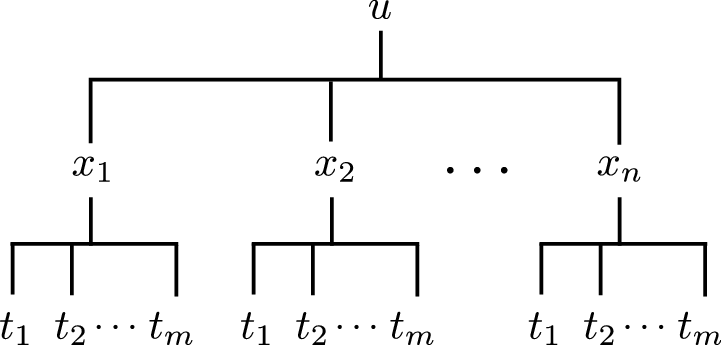
\includegraphics[width=0.500\linewidth]{chain3.png}\hfill}


\subsection{Dæmi}
\label{Kafli2:id23}
Látum \(T\) vera fall af fall af \(x\), \(y\) og \(t\),
og \(x\) og \(y\) föll af \(t\). Finnum
\(\frac{ dT}{dt}\).

{\hfill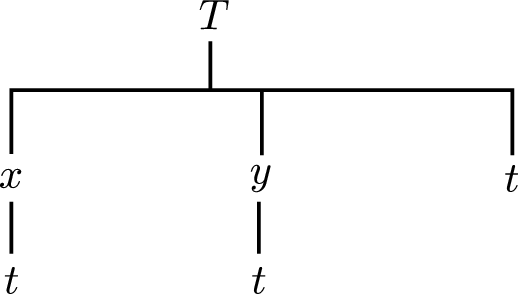
\includegraphics[width=0.400\linewidth]{chain5.png}\hfill}
\begin{gather}
\begin{split}\displaystyle \frac{d T}{d t} = \frac{\partial T}{\partial x} \frac{d x}{d t} +\frac{\partial T}{\partial y} \frac{d y}{d t} + \frac{\partial T}{\partial t} .\end{split}\notag
\end{gather}

\subsection{Dæmi}
\label{Kafli2:id24}
Látum \(T\) vera fall af fall af \(x\), \(y\), \(s\) og
\(t\), og \(x\) og \(y\) föll af \(s\) og \(t\).
Finnum \(\frac{ \partial T}{\partial t}\).

{\hfill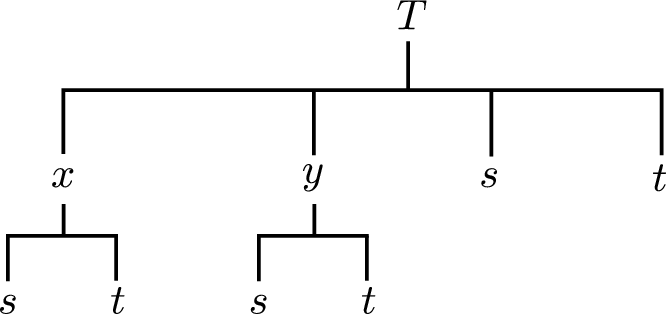
\includegraphics[width=0.500\linewidth]{chain6.png}\hfill}
\begin{gather}
\begin{split}\displaystyle \frac{\partial T}{\partial t} = \frac{\partial T}{\partial x} \frac{\partial x}{\partial t} +\frac{\partial T}{\partial y} \frac{\partial y}{\partial t} + \left(\frac{\partial T}{\partial t}\right)_{x,y,s} .\end{split}\notag
\end{gather}

\subsection{Dæmi}
\label{Kafli2:id25}
Látum \(z\) vera fall af fall af \(u\), \(v\) og \(r\),
\(u\) og \(v\) vera föll af \(x\), \(y\) og \(r\) og
\(r\) vera fall af \(x\) og \(y\). Skrifum niður
\(\frac{\partial z}{\partial x}\).

{\hfill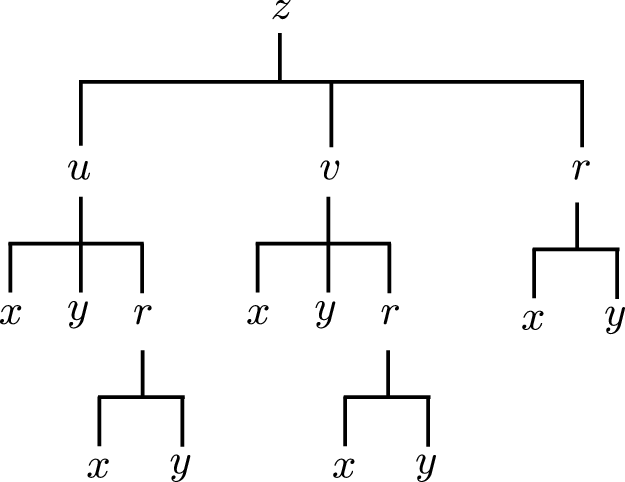
\includegraphics[width=0.400\linewidth]{chain4.png}\hfill}
\begin{gather}
\begin{split}\displaystyle\end{split}\notag\\\begin{split}\displaystyle\frac{\partial z}{\partial x} = \frac{\partial z}{\partial u} \frac{\partial u}{\partial x} +\frac{\partial z}{\partial u} \frac{\partial u}{\partial r} \frac{\partial r}{\partial x}
+ \frac{\partial z}{\partial v} \frac{\partial v}{\partial x} + \frac{\partial z}{\partial v} \frac{\partial v}{\partial r} \frac{\partial r}{\partial x} +\frac{\partial z}{\partial r} \frac{\partial r}{\partial x}.\end{split}\notag
\end{gather}

\section{Jákvætt einsleit föll}
\label{Kafli2:jakvaett-einsleit-foll}
\index{fall!jákvætt einsleitt fall}\index{jákvætt einsleitt fall}

\subsection{Skilgreining}
\label{Kafli2:index-13}\label{Kafli2:id26}
Fall \(f(x_1, x_2, \ldots, x_n)\) er sagt vera \emph{jákvætt einsleitt af
stigi} \(k\) (e. positively homogeneous of degree \(k\)) ef
fyrir sérhvern punkt \((x_1, x_2, \ldots, x_n)\) og sérhverja tölu
\(t>0\) gildir að
\begin{gather}
\begin{split}\displaystyle f(tx_1, tx_2, \ldots, tx_n)=t^kf(x_1, x_2, \ldots, x_n).\end{split}\notag
\end{gather}

\subsection{Setning}
\label{Kafli2:id27}
Ef fall \(f(x_1, x_2, \ldots, x_n)\) hefur samfelldar fyrsta stigs
hlutafleiður og er jákvætt einsleitt af stigi \(k\) þá er
\begin{gather}
\begin{split}\displaystyle \sum_{i=1}^n x_if_i(x_1, x_2, \ldots, x_n)=kf(x_1, x_2, \ldots, x_n).\end{split}\notag
\end{gather}

\section{Diffranleiki í einni breytistærð}
\label{Kafli2:diffranleiki-i-einni-breytistaer}

\subsection{Skilgreining}
\label{Kafli2:id28}
Látum \(f\) vera fall af einni breytistærð og gerum ráð fyrir að
\(f\) sé skilgreint á opnu bili sem inniheldur punktinn \(a\).
Fallið \(f\) er sagt vera \textit{diffranlegt} í punkti \(a\) ef
markgildið
\begin{gather}
\begin{split}\displaystyle f'(a)=\lim_{h\rightarrow 0}\frac{f(a+h)-f(a)}{h}\end{split}\notag
\end{gather}
er til.

\index{diffranleiki!falls af einni breytistærð}

\section{Diffranleiki í einni breytistærð - önnur lýsing}
\label{Kafli2:index-14}\label{Kafli2:diffranleiki-i-einni-breytistaer-onnur-lysing}

\subsection{Skilgreining}
\label{Kafli2:id29}
Látum \(f\) vera fall af einni breytistærð og gerum ráð fyrir að
\(f\) sé skilgreint á opnu bili sem inniheldur punktinn \(a\).
Fallið \(f\) er sagt vera \textit{diffranlegt} í punkti \(a\) ef til er
tala \(m\) þannig að ef \(L(x)=f(a)+m(x-a)\) þá er
\begin{gather}
\begin{split}\displaystyle \lim_{h\rightarrow 0}\frac{f(a+h)-L(a+h)}{h}=0.\end{split}\notag
\end{gather}
(Talan \(m\) verður að vera jöfn \(f'(a)\).)

Fallið \(f\) er ’nálægt’ línunni \(L\) nálægt punktinum
\(a\).


\section{Diffranleiki}
\label{Kafli2:diffranleiki}
\index{diffranleiki!falls af tveimur breytistærðum}

\subsection{Skilgreining}
\label{Kafli2:id30}\label{Kafli2:index-15}
Fall \(f(x,y)\) sem er skilgreint á opinni skífu umhverfis
\((a,b)\) er sagt vera \textit{diffranlegt} í punktinum \((a,b)\) ef
báðar fyrsta stigs hlutafleiður \(f\) eru skilgreindar í
\((a,b)\) og ef
\begin{gather}
\begin{split}\displaystyle\end{split}\notag\\\begin{split}\lim_{(h,k)\rightarrow (0,0)}
\frac{f(a+h, b+k)-S(a+h,b+k)}{\sqrt{h^2+k^2}}=0\end{split}\notag
\end{gather}
þar sem \(S(x,y) = f(a,b) + f_1(a,b)(x-a)+f_2(a,b)(y-b)\).

Fallið \(f\) er ’nálægt’ sléttunni \(S\) nálægt punktinum
\((a,b)\).

\index{snertiplan}

\section{Snertiplan}
\label{Kafli2:index-16}\label{Kafli2:id31}
Ef \(f\) er diffranlegt í \((a,b)\) þá kallast planið \(S\)
\textit{snertiplan} við graf fallsins.

{\hfill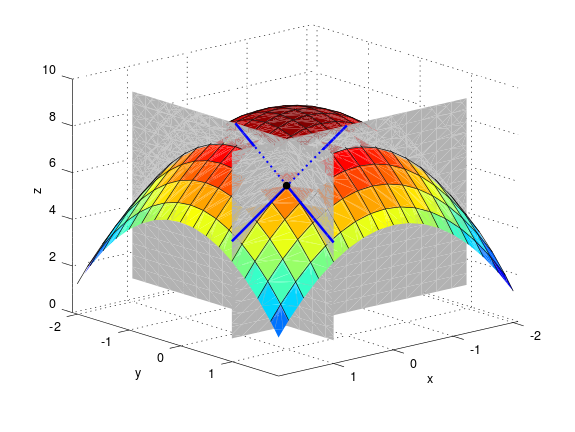
\includegraphics[width=0.600\linewidth]{bothpart.png}\hfill}

\(S(x,y) = f(a,b) + f_1(a,b)(x-a)+f_2(a,b)(y-b)\).


\section{Diffranleiki}
\label{Kafli2:id32}
\index{meðalgildissetningin}

\subsection{Setning (Meðalgildissetningin)}
\label{Kafli2:index-17}\label{Kafli2:setning-mealgildissetningin}
Gerum ráð fyrir að fallið \(f\) sé samfellt á lokaða bilinu
\([a,b]\) og diffranlegt á opna bilinu \((a,b)\). Þá er til
punktur \(c\) á opna bilinu \((a,b)\) þannig að
\begin{gather}
\begin{split}\displaystyle f(b)-f(a)=f'(c)(b-a).\end{split}\notag
\end{gather}

\subsection{Setning}
\label{Kafli2:id33}
Látum \(f(x,y)\) vera fall sem er skilgreint á opinni skífu
\(\cal D\) með miðju í \((a,b)\) þannig að á þessari skífu eru
báðar fyrsta stigs hlutafleiður \(f\) skilgreindar og samfelldar.
Gerum ráð fyrir að \(h\) og \(k\) séu tölur þannig að
\((x+h, y+k)\in{\cal D}\). Þá eru til tölur \(\theta_1\) og
\(\theta_2\) á milli 0 og 1 þannig að
\begin{gather}
\begin{split}\displaystyle f(a+h,b+k)-f(a,b)=hf_1(a+\theta_1h,b+k)+kf_2(a,b+\theta_2k).\end{split}\notag
\end{gather}

\subsection{Setning}
\label{Kafli2:id34}
Látum \(f(x,y)\) vera fall sem er skilgreint á opinni skífu
\(\cal D\) með miðju í \((a,b)\) þannig að á þessari skífu eru
báðar fyrsta stigs hlutafleiður \(f\) skilgreindar og samfelldar. Þá
er fallið \(f\) diffranlegt í \((a,b)\).


\subsection{Setning}
\label{Kafli2:id35}
Gerum ráð fyrir að \(f(x,y)\) sé fall sem er diffranlegt í punktinum
\((a,b)\). Þá er \(f\) samfellt í \((a,b)\).


\subsection{\textit{Keðjuregla}}
\label{Kafli2:id36}
Ritum \(z=f(x,y)\) þar sem \(x=x(s,t)\) og \(y=y(s,t)\).
Gerum ráð fyrir að
\begin{enumerate}
\item {} 
\(x(a,b)=p\) og \(y(a,b)=q\);

\item {} 
fyrsta stigs hlutafleiður \(x(s,t)\) og \(y(s,t)\) eru
skilgreindar í punktinum \((a,b)\);

\item {} 
fallið \(f\) er diffranlegt í punktinum \((p,q)\).

\end{enumerate}

Þá eru fyrsta stigs hlutafleiður \(z\) með tilliti til breytanna
\(s\) og \(t\) skilgreindar í punktinum \((a,b)\) og um þær
gildir að
\begin{gather}
\begin{split}\displaystyle\end{split}\notag\\\begin{split}\frac{\partial z}{\partial s}=
\frac{\partial z}{\partial x}\frac{\partial x}{\partial s}
+\frac{\partial z}{\partial y}\frac{\partial y}{\partial s}\end{split}\notag
\end{gather}
og
\begin{gather}
\begin{split}\displaystyle\end{split}\notag\\\begin{split}\frac{\partial z}{\partial t}=
\frac{\partial z}{\partial x}\frac{\partial x}{\partial t}
+\frac{\partial z}{\partial y}\frac{\partial y}{\partial t}.\end{split}\notag
\end{gather}

\section{Diffur}
\label{Kafli2:diffur}
\index{diffur}

\subsection{Skilgreining}
\label{Kafli2:index-18}\label{Kafli2:id37}
Ritum \(z=f(x_1, x_2, \ldots, x_n)\). \textit{Diffrið} af \(z\) er
skilgreint sem
\begin{gather}
\begin{split}\displaystyle\end{split}\notag\\\begin{split}dz=df=\frac{\partial z}{\partial x_1}dx_1
+\frac{\partial z}{\partial x_2}dx_2
+\cdots+\frac{\partial z}{\partial x_n}dx_n.\end{split}\notag
\end{gather}
Diffrið er nálgun á
\begin{gather}
\begin{split}\displaystyle\end{split}\notag\\\begin{split}\Delta f=f(x_1+dx_1, x_2+dx_2,\ldots,
x_n+dx_n)-f(x_1,x_2,\ldots,x_n).\end{split}\notag
\end{gather}

\section{Varpanir \(\mbox{${\bf R}^n$}\rightarrow\mbox{${\bf R}^m$}\)}
\label{Kafli2:varpanir}

\subsection{Táknmál}
\label{Kafli2:taknmal}
Látum
\(\mbox{${\bf f}$}:\mbox{${\bf R}^n$}\rightarrow\mbox{${\bf R}^m$}\)
tákna vörpun. Ritum \(\mbox{${\bf f}$}=(f_1,\ldots,f_m)\) þar sem
hvert \(f_i\) er fall
\(\mbox{${\bf R}^n$}\rightarrow{\mathbb  R}\). Fyrir punkt í
\(\mbox{${\bf R}^n$}\) ritum við
\(\mbox{${\bf x}$}=(x_1,x_2,\ldots,x_n)\). Síðan ritum við
\(\mbox{${\bf y}$}=\mbox{${\bf f}$}(\mbox{${\bf x}$})\) þar sem
\(\mbox{${\bf y}$}=(y_1,y_2,\ldots,y_m)\) og


\section{Jacobi-fylki}
\label{Kafli2:jacobi-fylki}
\index{Jacobi-!fylki}

\subsection{Skilgreining}
\label{Kafli2:id38}\label{Kafli2:index-19}
Notum táknmálið úr 2.22.1. Ef allar hlutafleiðurnar \(\partial
y_i/\partial x_j\) eru skilgreindar í punktinum \(\mbox{${\bf x}$}\)
þá skilgreinum við \emph{Jacobi-fylki} \(f\) í punktinum
\(\mbox{${\bf x}$}\) sem \(m\times n\) fylkið
\begin{gather}
\begin{split}\displaystyle\end{split}\notag\\\begin{split}D\mbox{${\bf f}$}(\mbox{${\bf x}$})=\begin{bmatrix}
\frac{\partial y_1}{\partial x_1}&\frac{\partial y_1}{\partial x_2}&
\cdots&\frac{\partial y_1}{\partial x_n}\\
\frac{\partial y_2}{\partial x_1}&\frac{\partial y_2}{\partial x_2}&
\cdots&\frac{\partial y_2}{\partial x_n}\\
\vdots&\vdots&\ddots&\vdots\\
\frac{\partial y_m}{\partial x_1}&\frac{\partial y_m}{\partial x_2}&
\cdots&\frac{\partial y_m}{\partial x_n}
\end{bmatrix}\end{split}\notag
\end{gather}
\index{diffranleiki!varpana}

\section{Diffranleiki varpana \(\mbox{${\bf R}^n$}\rightarrow\mbox{${\bf R}^m$}\)}
\label{Kafli2:diffranleiki-varpana}\label{Kafli2:index-20}

\subsection{Skilgreining}
\label{Kafli2:id39}
Notum táknmálið úr 2.22.1 og 2.23.1. Látum
\(\mbox{${\bf a}$}=(a_1, a_2, \ldots, a_n)\) vera fastan punkt í
\(\mbox{${\bf R}^n$}\) og ritum
\(\mbox{${\bf h}$}=(h_1,h_2,\ldots,h_n)\). Vörpunin
\(\mbox{${\bf f}$}\) er sögð diffranleg í punktinum
\(\mbox{${\bf a}$}\) ef
\begin{gather}
\begin{split}\displaystyle\end{split}\notag\\\begin{split}\lim_{\mbox{${\bf h}$}\rightarrow
  \mbox{${\bf 0}$}}\frac{|\mbox{${\bf f}$}(\mbox{${\bf a}$}+\mbox{${\bf h}$})-\mbox{${\bf f}$}(\mbox{${\bf a}$})-D\mbox{${\bf f}$}(\mbox{${\bf a}$})\mbox{${\bf h}$}|}{|\mbox{${\bf h}$}|}=0.\end{split}\notag
\end{gather}
Vörpunin \(f\) er ’nálægt’ línulegu vörpuninni
\(D\mbox{${\bf f}$}\) nálægt punktinum \(\mbox{${\bf a}$}\).

Línulega vörpunin \(D\mbox{${\bf f}$}\) kallast afleiða
\(\mbox{${\bf f}$}\).


\section{\textit{Keðjuregla}}
\label{Kafli2:id40}

\subsection{Setning}
\label{Kafli2:id41}
Látum
\(\mbox{${\bf f}$}:\mbox{${\bf R}^n$}\rightarrow \mbox{${\bf R}^m$}\)
og
\(\mbox{${\bf g}$}:\mbox{${\bf R}^m$}\rightarrow \mbox{${\bf R}^k$}\)
vera varpanir. Gerum ráð fyrir að vörpunin \(\mbox{${\bf f}$}\) sé
diffranleg í punkti \(\mbox{${\bf x}$}\) og vörpunin
\(\mbox{${\bf g}$}\) sé diffranleg í punktinum
\(\mbox{${\bf y}$}=\mbox{${\bf f}$}(\mbox{${\bf x}$})\). Þá er
samskeytta vörpunin
\(\mbox{${\bf g}$}\circ\mbox{${\bf f}$}:\mbox{${\bf R}^n$}\rightarrow\mbox{${\bf R}^k$}\)
diffranleg í \(\mbox{${\bf x}$}\) og
\begin{gather}
\begin{split}\displaystyle D(\mbox{${\bf g}$}\circ\mbox{${\bf f}$})(\mbox{${\bf x}$})=D\mbox{${\bf g}$}(\mbox{${\bf f}$}(\mbox{${\bf x}$}))D\mbox{${\bf f}$}(\mbox{${\bf x}$}).\end{split}\notag
\end{gather}
\index{stigull}

\section{Stigull}
\label{Kafli2:stigull}\label{Kafli2:index-21}

\subsection{Skilgreining}
\label{Kafli2:id42}
Látum \(f(x,y)\) vera fall og \((x,y)\) punkt þar sem báðar
fyrsta stigs hlutafleiður \(f\) eru skilgreindar. Skilgreinum
\textit{stigul} \(f\) í punktinum \((x,y)\) sem vigurinn
\begin{gather}
\begin{split}\displaystyle \nabla f(x,y)=f_1(x,y)\mbox{${\bf i}$}+f_2(x,y)\mbox{${\bf j}$}.\end{split}\notag
\end{gather}
\textit{Stigull} \(f\) er stundum táknaður með \textbf{grad}\(\,f\).


\subsection{Ritháttur}
\label{Kafli2:id43}
Oft hentugt að rita
\begin{gather}
\begin{split}\displaystyle \nabla=\mbox{${\bf i}$}\frac{\partial}{\partial x}+ \mbox{${\bf j}$}\frac{\partial}{\partial y}.\end{split}\notag
\end{gather}
Þá er litið svo á að \(\nabla\) sé \textit{diffurvirki},
þ.e.a.s. \(\nabla\) gefur fyrirmæli um hvað á að gera við
\(f\) til að fá \(\nabla f(x,y)\).


\section{Dæmi}
\label{Kafli2:id44}
{\hfill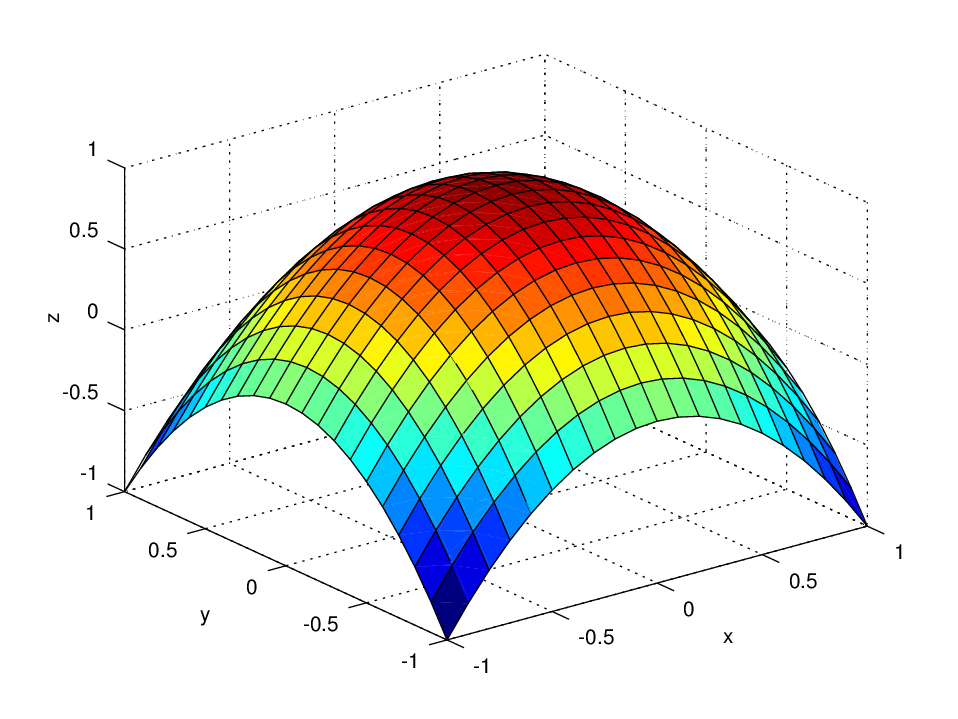
\includegraphics[width=0.600\linewidth]{gradfurf.png}\hfill}

\emph{Graf} \(z=1-x^2-y^2\)

{\hfill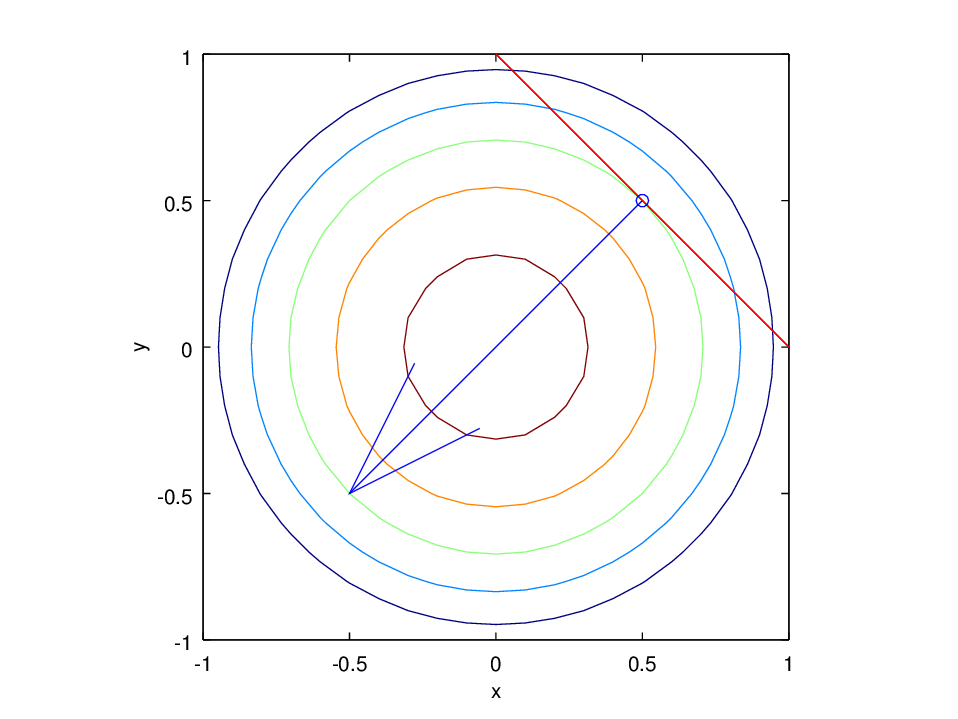
\includegraphics[width=0.600\linewidth]{gradient.png}\hfill}

\emph{Jafnhæðarlínur} \(z=1-x^2-y^2\). \emph{Stigull og snertilína við jafnhæðarlínuna} \(z=0.5\) \emph{í} \((x,y) = (0.5,0.5)\).


\subsection{Setning}
\label{Kafli2:id45}
Gerum ráð fyrir að fallið \(f(x,y)\) sé diffranlegt í punktinum
\((a,b)\) og að \(\nabla f(a,b) \neq \mathbf{0}\). Þá er
vigurinn \(\nabla f(a,b)\) hornréttur á þá jafnhæðarlínu \(f\)
sem liggur í gegnum punktinn \((a,b)\).

\index{snertilína!við jafnhæðarferil}

\section{Snertilína við jafnhæðarferil}
\label{Kafli2:snertilina-vi-jafnhaearferil}\label{Kafli2:index-22}

\subsection{Setning}
\label{Kafli2:id46}
Gerum ráð fyrir að fallið \(f(x,y)\) sé diffranlegt í punktinum
\((a,b)\) og að \(\nabla f(a,b) \neq \mathbf{0}\). Jafna
\textit{snertilínu} við \textit{jafnhæðarferil} \(f\) í punktinum \((a,b)\) er
gefin með formúlunni
\begin{gather}
\begin{split}\displaystyle \nabla f(a,b)\cdot (x,y)=\nabla f(a,b)\cdot (a,b),\end{split}\notag
\end{gather}
eða
\begin{gather}
\begin{split}\displaystyle f_1(a,b)(x-a)+f_2(a,b)(y-b)=0.\end{split}\notag
\end{gather}
\index{stefnuafleiða}

\section{Stefnuafleiða}
\label{Kafli2:index-23}\label{Kafli2:stefnuafleia}

\subsection{Skilgreining}
\label{Kafli2:id47}
Látum \(\mbox{${\bf u}$}=u\mbox{${\bf i}$}+v\mbox{${\bf j}$}\) vera
einingarvigur. \textit{Stefnuafleiða} \(f\) í punktinum \((a,b)\) í
stefnu \(\mbox{${\bf u}$}\) er skilgreind sem
\begin{gather}
\begin{split}\displaystyle D_{\mbox{${\bf u}$}}f(a,b)=\lim_{h\rightarrow 0^+}\frac{f(a+hu, b+hv)-f(a,b)}{h}\end{split}\notag
\end{gather}
ef markgildið er skilgreint.

\begin{notice}{warning}{Aðvörun:}
Í skilgreiningunni á stefnuafleiðu er tekið einhliða markgildi. Berið það saman við skilgreiningu á hlutafleiðu þar sem markgildið er tvíhliða.
\end{notice}


\subsection{Setning}
\label{Kafli2:id48}
Gerum ráð fyrir að fallið \(f\) sé diffranlegt í \((a,b)\) og
\(\mbox{${\bf u}$}=u\mbox{${\bf i}$}+v\mbox{${\bf j}$}\) sé
einingarvigur. Þá er stefnuafleiðan í punktinum \((a,b)\) í stefnu
\(\mbox{${\bf u}$}\) skilgreind og gefin með formúlunni
\begin{gather}
\begin{split}\displaystyle D_{\mbox{${\bf u}$}}f(a,b)=\mbox{${\bf u}$}\cdot \nabla f(a,b).\end{split}\notag
\end{gather}

\subsection{Setning}
\label{Kafli2:id49}
Látum \(f\) vera gefið fall og gerum ráð fyrir að \(f\) sé
diffranlegt í punktinum \((a,b)\).

(a) Hæsta gildið á stefnuafleiðunni \(D_{\mbox{${\bf u}$}}f(a,b)\)
fæst þegar \(\mbox{${\bf u}$}\) er einingarvigur í stefnu
\(\nabla f(a,b)\), þ.e.a.s.
\(\mbox{${\bf u}$}=\frac{\nabla f(a,b)}{|\nabla f(a,b)|}\).

(b) Lægsta gildið á stefnuafleiðunni \(D_{\mbox{${\bf u}$}}f(a,b)\)
fæst þegar \(\mbox{${\bf u}$}\) er einingarvigur í stefnu
\(-\nabla f(a,b)\), þ.e.a.s.
\(\mbox{${\bf u}$}=-\frac{\nabla f(a,b)}{|\nabla f(a,b)|}\).

(c) Ef \(\cal C\) er sú hæðarlína \(f\) sem liggur í gegnum
\((a,b)\) og \(\mbox{${\bf u}$}\) er einingarsnertivigur við
\(\cal C\) í punktinum \((a,b)\) þá er
\(D_{\mbox{${\bf u}$}}f(a,b)=0\).

{\hfill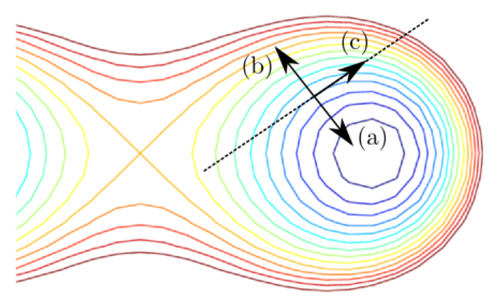
\includegraphics[width=0.500\linewidth]{contours.png}\hfill}


\subsection{Setning}
\label{Kafli2:id50}
Látum \(f\) vera gefið fall og gerum ráð fyrir að \(f\) sé
diffranlegt í punktinum \((a,b)\).

(a) Í punktinum \((a,b)\) þá vex \(f\) hraðast ef haldið er í
stefnu \(\nabla f(a,b)\).

(b) Í punktinum \((a,b)\) þá minnkar \(f\) hraðast ef haldið er
í stefnu \(-\nabla f(a,b)\).

(c) Ef \(\cal C\) er sú hæðarlína \(f\) sem liggur í gegnum
\((a,b)\) og \(\mbox{${\bf u}$}\) er einingarsnertivigur við
\(\cal C\) í punktinum \((a,b)\) þá er er vaxtarhraði \(f\)
í stefnu \(\mbox{${\bf u}$}\) jafn 0.


\section{Stigull (aftur)}
\label{Kafli2:stigull-aftur}

\subsection{Skilgreining}
\label{Kafli2:id51}
Látum \(f\) vera fall af þremur breytistærðum, þannig að allar þrjár
fyrsta stigs hlutafleiður \(f\) í punktinum \((x,y,z)\) séu
skilgreindar. \textit{Stigull} \(f\) í punktinum \((x,y,z)\) er
skilgreindur sem vigurinn
\begin{gather}
\begin{split}\displaystyle \nabla f(x,y,z)=f_1(x,y,z)\mbox{${\bf i}$}+f_2(x,y,z)\mbox{${\bf j}$}+f_3(x,y,z)\mbox{${\bf k}$}.\end{split}\notag
\end{gather}
\index{snertiplan!við jafnhæðarflöt}

\section{Snertiplan við jafnhæðarflöt}
\label{Kafli2:snertiplan-vi-jafnhaearflot}\label{Kafli2:index-24}

\subsection{Setning}
\label{Kafli2:id52}
Látum \(f\) vera fall af þremur breytistærðum þannig að fallið
\(f\) er diffranlegt í punktinum \((a,b,c)\). Látum
\(\cal F\) tákna þann \textit{jafnhæðarflöt} \(f\) sem liggur um
\((a,b,c)\). Stigullinn \(\nabla f(a,b,c)\) er hornréttur á
flötinn \(\cal F\) í punktinum \((a,b,c)\) og \textit{snertiplan} (ef
\(\nabla f(a,b,c)\neq\mbox{${\bf 0}$}\)) við jafnhæðarflötinn í
punktinum \((a,b,c)\) er gefið með jöfnunni
\begin{gather}
\begin{split}\displaystyle \nabla f(a,b,c)\cdot(x,y,z)=\nabla f(a,b,c)\cdot(a,b,c)\end{split}\notag
\end{gather}
eða með umritun
\begin{gather}
\begin{split}\displaystyle f_1(a,b,c)(x-a)+f_2(a,b,c)(y-b)+f_3(a,b,c)(z-c)=0.\end{split}\notag
\end{gather}

\section{Fólgin föll og Taylor-nálganir}
\label{Kafli2:folgin-foll-og-taylor-nalganir}
\index{fólgið fall}\index{fall!fólgið fall}

\subsection{Upprifjun}
\label{Kafli2:index-25}\label{Kafli2:upprifjun}
Skoðum feril sem gefinn er með jöfnu \(F(x,y)=0\) og gerum ráð fyrir
að báðar fyrsta stigs hlutafleiður \(F\) séu samfelldar. Látum
\((x_0,y_0)\) vera punkt á ferlinum. Ef \(F_2(x_0,y_0)\neq 0\)
þá má skoða \(y\) sem fall af \(x\) í grennd við punktinn
\((x_0,y_0)\) og fallið \(y=y(x)\) er diffranlegt í punktinum
\(x_0\) og afleiðan er gefin með formúlunni
\begin{gather}
\begin{split}\displaystyle y'(x_0)=-\frac{F_1(x_0,y_0)}{F_2(x_0,y_0)}.\end{split}\notag
\end{gather}
Sagt að jafnan \(F(x,y)=0\) skilgreini \(y\) sem \textit{fólgið fall}
af \(x\) í grennd við \((x_0,y_0)\).


\subsection{Setning}
\label{Kafli2:id53}
Látum \(F\) vera fall af \(n\)-breytum \(x_1, \ldots,
x_n\) og gerum ráð fyrir að allar fyrsta stigs hlutafleiður \(F\) séu
samfelldar. Látum \((a_1,\ldots,a_n)\) vera punkt þannig að
\(F(a_1,\ldots,a_n)=0\). Ef \(F_n(a_1,\ldots,a_n)\neq 0\) þá er
til samfellt diffranlegt fall \(\varphi(x_1, \ldots, x_{n-1})\)
skilgreint á opinni kúlu \(B\) utan um \((a_1,\ldots,a_{n-1})\)
þannig að
\begin{gather}
\begin{split}\displaystyle \varphi(a_1,\ldots,a_{n-1})=a_n\end{split}\notag
\end{gather}
og
\begin{gather}
\begin{split}\displaystyle F(x_1,\ldots, x_{n-1}, \varphi(x_1, \ldots, x_{n-1}))=0\end{split}\notag
\end{gather}
fyrir alla punkta \((x_1, \ldots, x_{n-1})\) í \(B\).

Ennfremur gildir að
\begin{gather}
\begin{split}\displaystyle\end{split}\notag\\\begin{split}\varphi_i(a_1,\ldots,a_{n-1})
=-\frac{F_i(a_1,\ldots,a_n)}{F_n(a_1,\ldots,a_n)}.\end{split}\notag
\end{gather}
\index{Jacobi-!ákveða}

\subsection{Skilgreining}
\label{Kafli2:index-26}\label{Kafli2:id54}
\textit{Jacobi-ákveða} tveggja falla \(u=u(x,y)\) og \(v=v(x,y)\) með
tilliti til breytanna \(x\) og \(y\) er skilgreind sem
\begin{gather}
\begin{split}\displaystyle\end{split}\notag\\\begin{split}\frac{\partial(u,v)}{\partial(x,y)}=
\begin{vmatrix}
\frac{\partial u}{\partial x}&\frac{\partial u}{\partial y}\\
\frac{\partial v}{\partial x}&\frac{\partial v}{\partial y}
\end{vmatrix}.\end{split}\notag
\end{gather}
Ef \(F\) og \(G\) eru föll af breytum \(x,y,z,\ldots\) þá
skilgreinum við, til dæmis,
\begin{gather}
\begin{split}\displaystyle\end{split}\notag\\\begin{split}\frac{\partial(F,G)}{\partial(x,y)}=
\begin{vmatrix}
\frac{\partial F}{\partial x}&\frac{\partial F}{\partial y}\\
\frac{\partial G}{\partial x}&\frac{\partial G}{\partial y}
\end{vmatrix}\quad \mbox{og}\quad
\frac{\partial(F,G)}{\partial(y,z)}=
\begin{vmatrix}
\frac{\partial F}{\partial y}&\frac{\partial F}{\partial z}\\
\frac{\partial G}{\partial y}&\frac{\partial G}{\partial z}
\end{vmatrix}.\end{split}\notag
\end{gather}
Ef við höfum föll \(F, G, H\) af breytum \(x,y,z,w,\ldots\) þá
skilgreinum við, til dæmis,
\begin{gather}
\begin{split}\displaystyle\end{split}\notag\\\begin{split}\frac{\partial(F,G,H)}{\partial(w,z,y)}=
\begin{vmatrix}
\frac{\partial F}{\partial w}&\frac{\partial F}{\partial z}
&\frac{\partial F}{\partial y}\\
\frac{\partial G}{\partial w}&\frac{\partial G}{\partial z}
&\frac{\partial G}{\partial y}\\
\frac{\partial H}{\partial w}&\frac{\partial H}{\partial z}
&\frac{\partial H}{\partial y}
\end{vmatrix}.\end{split}\notag
\end{gather}
\index{Cramer}

\subsection{Setning (Upprifjun á reglu Cramers.)}
\label{Kafli2:index-27}\label{Kafli2:setning-upprifjun-a-reglu-cramers}
Látum \(A\) vera andhverfanlegt \(n\times n\) fylki og
\(\mbox{${\bf b}$}\) vigur í \(\mbox{${\bf R}^n$}\). Gerum ráð
fyrir að \(\mbox{${\bf x}$}=(x_1, x_2, \ldots, x_n)\) sé lausn á
\(A\mbox{${\bf x}$}=\mbox{${\bf b}$}\). Skilgreinum \(B_i\) sem
\(n\times n\) fylkið sem fæst með því að setja vigurinn
\(\mbox{${\bf b}$}\) í staðinn fyrir dálk \(i\) í \(A\). Þá
er
\begin{gather}
\begin{split}\displaystyle x_i=\frac{\det B_i}{\det A}.\end{split}\notag
\end{gather}
\index{setning!um fólgin föll}\index{fólgið fall!setning}

\subsection{Setning (\textit{Setningin um fólgin föll})}
\label{Kafli2:id55}\label{Kafli2:index-28}
Skoðum jöfnuhneppi
\begin{gather}
\begin{split}\displaystyle\end{split}\notag\\\begin{split}\begin{aligned}
F_{(1)}(x_1,\ldots,x_m, y_1, \ldots, y_n)&=0\\
F_{(2)}(x_1,\ldots,x_m, y_1, \ldots, y_n)&=0\\
\vdots\\
F_{(n)}(x_1,\ldots,x_m, y_1, \ldots, y_n)&=0.\end{aligned}\end{split}\notag
\end{gather}
Látum \(P_0=(a_1,\ldots, a_m, b_1,\ldots, b_n)\) vera punkt sem
uppfyllir jöfnurnar. Gerum ráð fyrir að allar fyrsta stigs hlutafleiður
fallanna \(F_{(1)},\ldots, F_{(n)}\) séu samfelldar á opinni kúlu
umhverfis \(P_0\) og að
\begin{gather}
\begin{split}\displaystyle\end{split}\notag\\\begin{split}\frac{\partial(F_{(1)}, \ldots, F_{(n)})}
{\partial( y_1, \ldots, y_n)}\,\bigg|_{P_0}\neq 0.\end{split}\notag
\end{gather}
\begin{DUlineblock}{0em}
\item[] \(\text{Þá eru til föll} \qquad \varphi_1(x_1,\ldots,x_m),\ldots,\varphi_n(x_1,\ldots,x_m)\)
\item[] á opinni kúlu \(B\) umhverfis \((a_1,\ldots,a_m)\) þannig að
\end{DUlineblock}
\begin{gather}
\begin{split}\displaystyle \varphi_1(a_1,\ldots,a_m)=b_1,\ldots,\varphi_n(a_1,\ldots,a_m)=b_n \qquad \text{og}\end{split}\notag
\end{gather}\begin{gather}
\begin{split}\displaystyle\end{split}\notag\\\begin{split}\begin{aligned}
F_{(1)}(x_1,\ldots,x_m, \varphi_1(x_1,\ldots,x_m),\ldots,
\varphi_n(x_1,\ldots,x_m))&=0\\
F_{(2)}(x_1,\ldots,x_m, \varphi_1(x_1,\ldots,x_m),\ldots,
\varphi_n(x_1,\ldots,x_m))&=0\\
\vdots\\
F_{(n)}(x_1,\ldots,x_m, \varphi_1(x_1,\ldots,x_m),\ldots,
\varphi_n(x_1,\ldots,x_m))&=0\end{aligned}\end{split}\notag
\end{gather}
fyrir alla punkta \((x_1,\ldots,x_m)\) í \(B\). Enn fremur fæst
að
\begin{gather}
\begin{split}\displaystyle\end{split}\notag\\\begin{split}\frac{\partial \varphi_i}{\partial x_j}
=\frac{\partial y_i}{\partial x_j}
=-\frac{\frac{\partial(F_{(1)}, \ldots, F_{(n)})}
{\partial( y_1, \ldots,x_j,\ldots y_n)}}
{\frac{\partial(F_{(1)}, \ldots, F_{(n)})}{\partial( y_1, \ldots, y_n)}}.\end{split}\notag
\end{gather}
\index{setning!um staðbundna andhverfu}

\subsection{Setning (Setningin um staðbundna andhverfu)}
\label{Kafli2:index-29}\label{Kafli2:setning-setningin-um-stabundna-andhverfu}
\begin{DUlineblock}{0em}
\item[] Látum
\end{DUlineblock}
\begin{gather}
\begin{split}\displaystyle\end{split}\notag\\\begin{split}\mbox{${\bf f}$}(x_1,\ldots,
x_n)=(f_1(x_1,\ldots,x_n),\ldots,f_n(x_1,\ldots,x_n))\end{split}\notag
\end{gather}
vera vörpun af \(n\) breytistærðum sem tekur gildi í
\(\mbox{${\bf R}^n$}\) og er skilgreind á opnu mengi í
\(\mbox{${\bf R}^n$}\). Gerum ráð fyrir að allar fyrsta stigs
hlutafleiður fallanna \(f_1, \ldots, f_n\) séu samfelld föll. Ef
Jacobi-fylkið \(D\mbox{${\bf f}$}(\mbox{${\bf x}$}_0)\) er
andhverfanlegt í punkti \(\mbox{${\bf x}$}_0\) á skilgreiningarsvæði
\(\mbox{${\bf f}$}\) þá er til opin kúla
\(B_{\mbox{${\bf x}$}}\) utan um \(\mbox{${\bf x}$}_0\) og opin
kúla \(B_{\mbox{${\bf y}$}}\) utan um
\(\mbox{${\bf y}$}_0=f(\mbox{${\bf x}$}_0)\) og vörpun
\textbar{} \(\mbox{${\bf g}$}:B_{\mbox{${\bf y}$}}\rightarrow B_{\mbox{${\bf x}$}}\)
þannig að
\(\mbox{${\bf g}$}(\mbox{${\bf f}$}(\mbox{${\bf x}$}))=\mbox{${\bf x}$}\)
fyrir alla punkta \(\mbox{${\bf x}$}\in B_{\mbox{${\bf x}$}}\) og
\(\mbox{${\bf f}$}(\mbox{${\bf g}$}(\mbox{${\bf y}$}))=\mbox{${\bf y}$}\)
fyrir alla punkta \(\mbox{${\bf y}$}\in B_{\mbox{${\bf y}$}}\).

\index{Taylor-!regla í einni breytistærð}

\subsection{Upprifjun (Taylor-regla í einni breytistærð.)}
\label{Kafli2:upprifjun-taylor-regla-i-einni-breytistaer}\label{Kafli2:index-30}
Látum \(f\) vera \(n+1\)-diffranlegt fall af einni breytistærð.
Margliðan
\begin{gather}
\begin{split}\displaystyle\end{split}\notag\\\begin{split}P_{(n)}(x)=f(a)+f'(a)(x-a)+\frac{f''(a)}{2!}(x-a)^2
+\cdots+\frac{f^{(n)}(a)}{n!}(x-a)^n\end{split}\notag
\end{gather}
kallast \(n\)\emph{-ta stigs Taylor-margliða} \(f\) \emph{með miðju í}
\(a\). Til er punktur \(s\) á milli \(a\) og \(x\)
þannig að
\begin{gather}
\begin{split}\displaystyle E_{(n)}(x)=f(x)-P_{(n)}(x)=\frac{f^{(n+1)}(s)}{(n+1)!}(x-a)^{n+1}.\end{split}\notag
\end{gather}
Fáum svo að
\begin{gather}
\begin{split}\displaystyle\end{split}\notag\\\begin{split}\begin{aligned}
&f(x)=P_{(n)}(x)+E_{(n)}(x) \\
&=f(a)+f'(a)(x-a)+\cdots+\frac{f^{(n)}(a)}{n!}(x-a)^n
+\frac{f^{(n+1)}(s)}{(n+1)!}(x-a)^{n+1}, \end{aligned}\end{split}\notag
\end{gather}
sem er kallað \(n\)\emph{-ta stigs Taylor-formúla.}

\index{Taylor-!margliða}

\subsection{Skilgreining}
\label{Kafli2:id56}\label{Kafli2:index-31}
Látum \(f(x,y)\) vera fall þannig að fyrsta stigs hlutafleiður
\(f\) eru skilgreindar og samfelldar. Margliðan
\begin{gather}
\begin{split}\displaystyle P_{(1)}(x,y)=f(a,b)+f_1(a,b)(x-a)+f_2(a,b)(y-b)\end{split}\notag
\end{gather}
kallast \emph{fyrsta stigs Taylor-margliða} \(f\) \emph{með miðju í}
\((a,b)\).


\subsection{Skilgreining}
\label{Kafli2:id57}
Látum \(f(x,y)\) vera fall þannig að fyrsta og annars stigs
hlutafleiður \(f\) eru skilgreindar og samfelldar. Margliðan
\begin{gather}
\begin{split}\displaystyle\end{split}\notag\\\begin{split}\begin{aligned}
P_{(2)}&(x,y)=f(a,b)+f_1(a,b)(x-a)+f_2(a,b)(y-b)\\
&+\frac{1}{2}\big(f_{11}(a,b)(x-a)^2+
2f_{12}(a,b)(x-a)(y-b)+f_{22}(a,b)(y-b)^2\big)\end{aligned}\end{split}\notag
\end{gather}
kallast \emph{annars stigs Taylor-margliða} \(f\) \emph{með miðju í}
\((a,b)\).


\subsection{Skilgreining og athugasemd}
\label{Kafli2:skilgreining-og-athugasemd}
Skilgreinum tvo \textit{diffurvirkja} \(D_1\) og \(D_2\) þannig að
\begin{gather}
\begin{split}\displaystyle\end{split}\notag\\\begin{split}D_1f(a,b)=f_1(a,b)\qquad\mbox{og}\qquad
D_2f(a,b)=f_2(a,b).\end{split}\notag
\end{gather}
Athugið að ef hlutafleiður \(f\) af nógu háum stigum eru allar
skilgreindar og samfelldar þá er \(D_1D_2=D_2D_1\), þ.e.a.s. ekki
skiptir máli í hvaða röð er diffrað, bara hve oft er diffrað með tilliti
til hvorrar breytu.

\index{tvíliðuregla}

\subsection{Upprifjun (\textit{Tvíliðuregla})}
\label{Kafli2:index-32}\label{Kafli2:id58}
Skilgreinum
\begin{gather}
\begin{split}\displaystyle {n\choose j}=\frac{n!}{j!(n-j)!}.\end{split}\notag
\end{gather}
Talan \({n\choose j}\) (lesið \(n\) yfir \(j\)) er
\(j+1\) talan í \(n+1\) línu Pascals-þríhyrningsins. Höfum að
\begin{gather}
\begin{split}\displaystyle (x+y)^n=\sum_{j=0}^n \textstyle{n\choose j}x^jy^{n-j}.\end{split}\notag
\end{gather}

\subsection{Regla}
\label{Kafli2:regla}
Ef \(f(x,y)\) er fall þannig að allar hlutafleiður af \(n\)-ta
og lægri stigum eru samfelldar þá gildir að
\begin{gather}
\begin{split}\displaystyle\end{split}\notag\\\begin{split}(hD_1+kD_2)^nf(a,b)=\sum_{j=0}^n \textstyle{n\choose j}
h^jk^{n-j}D_1^jD_2^{n-j}f(a,b).\end{split}\notag
\end{gather}

\subsection{Skilgreining}
\label{Kafli2:id59}
Fyrir fall \(f(x,y)\) þannig að allar hlutafleiður af \(n\)-ta
og lægri stigum eru samfelldar þá er \(n\)\emph{-ta stigs
Taylor-margliða} \(f\) \emph{með miðju í punktinum} \((a,b)\)
skilgreind sem margliðan
\begin{gather}
\begin{split}\displaystyle\end{split}\notag\\\begin{split}\begin{aligned}
P_{(n)}(x,y)&= \sum_{m=0}^n \frac{1}{m!}((x-a)D_1+(y-b)D_2)^m f(a,b)\\
&=\sum_{m=0}^n\sum_{j=0}^m \frac{1}{m!}\textstyle{m\choose j}
D_1^jD_2^{m-j}f(a,b)(x-a)^j(y-b)^{m-j}\\
&=\sum_{m=0}^n\sum_{j=0}^m \frac{1}{j!(m-j)!}
D_1^jD_2^{m-j}f(a,b)(x-a)^j(y-b)^{m-j}.\end{aligned}\end{split}\notag
\end{gather}

\subsection{Setning}
\label{Kafli2:id60}
Fyrir fall \(f(x,y)\) þannig að allar hlutafleiður af \(n+1\)-ta
og lægri stigum eru samfelldar þá gildir um skekkjuna í \(n\)-ta
stigs Taylor-nálgun að til er tala \(\theta\) á milli 0 og 1 þannig
að ef \(h=x-a\) og \(k=y-b\) þá er
\begin{gather}
\begin{split}\displaystyle\end{split}\notag\\\begin{split}f(x,y)-P_{(n)}(x,y)=\frac{1}{(n+1)!}(hD_1+kD_2)^{n+1}
f(a+\theta h, b+\theta k).\end{split}\notag
\end{gather}

\chapter{Útgildisverkefni}
\label{Kafli3::doc}\label{Kafli3:utgildisverkefni}
\emph{Old stories are like old friends, she used to say. You have to visit them from time to time.}

-George R.R. Martin, A Storm of Swords

\index{útgildi}\index{lággildi!staðbundið lággildi}\index{hágildi!staðbundið hágildi}\index{útgildi!staðbundið útgildi}\index{hæsta gildi}

\section{Útgildi}
\label{Kafli3:utgildi}\label{Kafli3:index-0}

\subsection{Skilgreining}
\label{Kafli3:skilgreining}
Látum \(f\) vera fall af tveim breytum skilgreint á mengi
\({\cal D}(f)\).

Sagt er að \(f\) hafi \textit{staðbundið lággildi} í
punkti \((a,b)\) ef til er tala \(r>0\) þannig að
\(f(a,b)\leq f(x,y)\) fyrir alla punkta
\((x,y)\in B_r(a,b)\cap{\cal D}(f)\).

Sagt er að \(f\) hafi \textit{staðbundið hágildi}  í
punkti \((a,b)\) ef til er tala \(r>0\) þannig að
\(f(a,b)\geq f(x,y)\) fyrir alla punkta
\((x,y)\in B_r(a,b)\cap{\cal D}(f)\).

Í þeim punktum þar sem \(f\) tekur annað hvort staðbundið lággildi
eða staðbundið hágildi er sagt að \(f\) hafi \textit{staðbundið útgildi}

Ef \(f(a,b)\leq f(x,y)\) fyrir alla punkta
\((x,y)\in {\cal D}(f)\) þá er sagt að \(f\) taki \emph{lægsta gildi}
í \((a,b)\) (e. global minimum). Ef \(f(a,b)\geq f(x,y)\) fyrir
alla punkta \((x,y)\in {\cal D}(f)\) þá er sagt að \(f\) taki
\textit{hæsta gildi} í \((a,b)\).

\index{útgildi!staðbundið útgildi}\index{stöðupunktur}

\section{Staðbundið útgildi}
\label{Kafli3:index-1}\label{Kafli3:stabundi-utgildi}

\subsection{Upprifjun}
\label{Kafli3:upprifjun}
Látum \(f\) vera fall af einni breytu skilgreint á mengi
\({\cal D}(f)\subseteq {\mathbb  R}\). Ef fallið \(f\) hefur
staðbundið útgildi í punkti \(a\) þá gildir eitt af þrennu um
\(a\):
\begin{enumerate}
\item {} 
\(f'(a)=0\). (punkturinn \(a\) kallast \textit{stöðupunktur}
\(f\)).

\item {} 
Afleiðan \(f'(a)\) er ekki skilgreind.

\item {} 
Punkturinn \(a\) er \textit{jaðarpunktur} \({\cal D}(f)\).

\end{enumerate}


\subsection{Setning}
\label{Kafli3:setning}
Látum \(f\) vera fall af tveim breytum skilgreint á mengi
\({\cal D}(f)\subseteq {\mathbb  R}^2\). Ef fallið \(f\) hefur
\textit{staðbundið útgildi} í punkti \((a,b)\) þá gildir eitt af þrennu um
\(a\)
\begin{enumerate}
\item {} 
\(\nabla f(a,b)=\mbox{${\bf 0}$}\). (punkturinn \((a,b)\)
kallast \textit{stöðupunktur} \(f\))

\item {} 
\textit{Stigullinn} \(\nabla f(a,b)\) er ekki skilgreindur.

\item {} 
Punkturinn \((a,b)\) er \textit{jaðarpunktur} \({\cal D}(f)\).

\end{enumerate}


\subsection{Dæmi}
\label{Kafli3:daemi}
Föll skilgreind á svæðinu \(-0.5 \leq x \leq 0.5\),
\(-0.5 \leq y \leq 0.5\). Hvar eru staðbundin hágildi?

{\hfill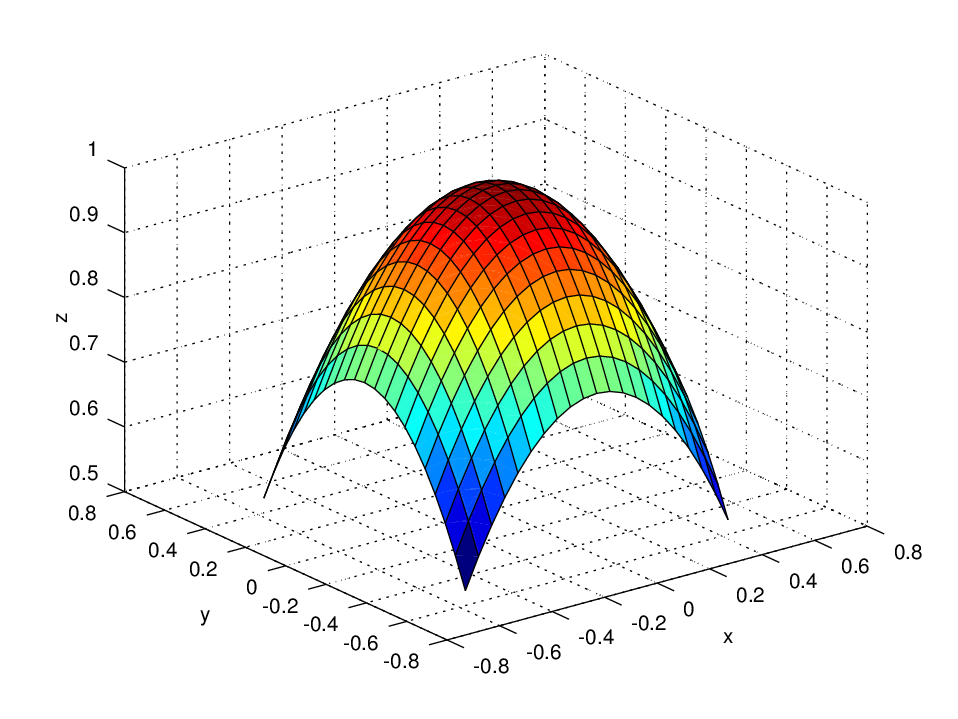
\includegraphics[width=0.600\linewidth]{peak_smooth.png}\hfill}

\(z = f(x,y) = 1-x^2-y^2\).

{\hfill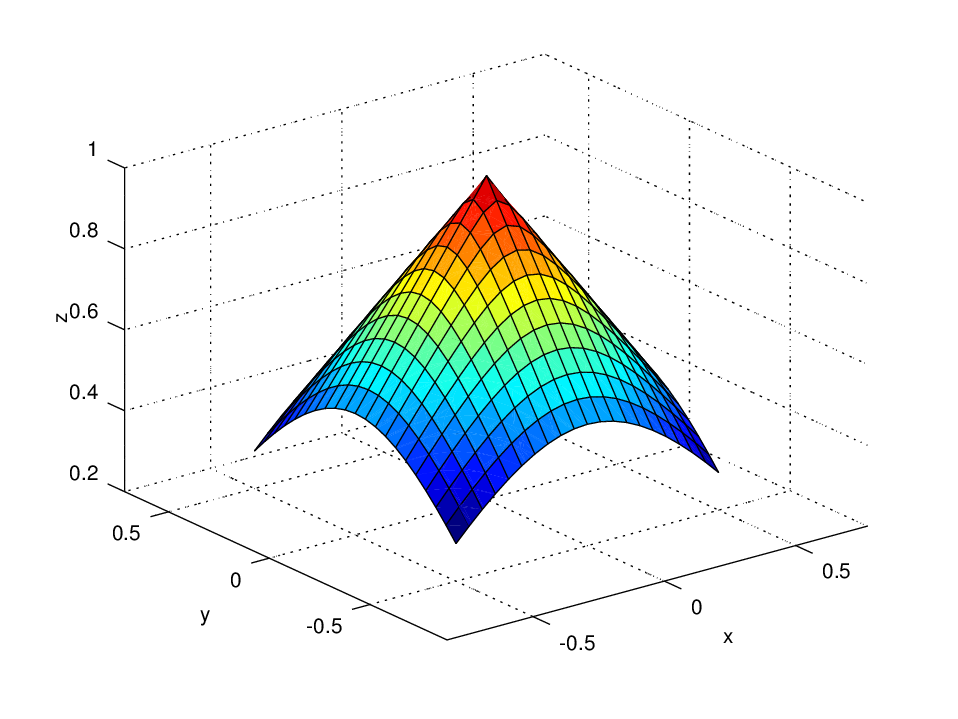
\includegraphics[width=0.600\linewidth]{peak.png}\hfill}

\(z = f(x,y) = 1-\sqrt{x^2+y^2}\).

{\hfill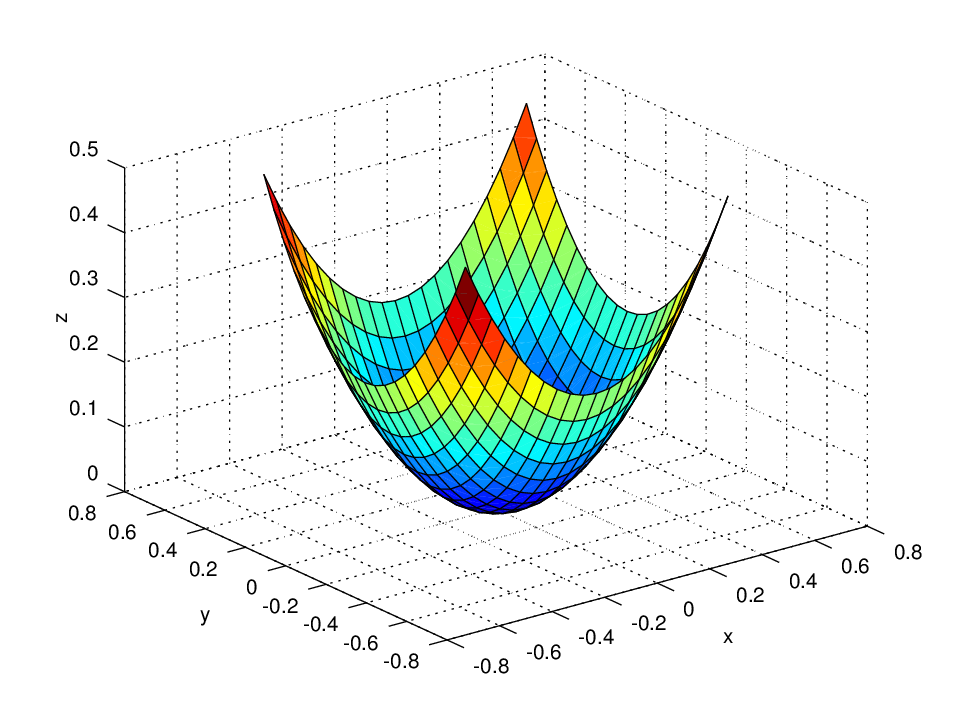
\includegraphics[width=0.600\linewidth]{max_bound.png}\hfill}

\(z= f(x,y) = x^2+y^2\).


\section{Tilvist útgilda}
\label{Kafli3:tilvist-utgilda}

\subsection{Setning}
\label{Kafli3:id1}
Látum \(f\) vera samfellt fall af tveim breytum skilgreint á lokuðu
og takmörkuðu mengi \({\cal D}(f)\). Fallið \(f\) tekur þá bæði
hæsta og lægsta gildi.

\index{söðulpunktur}

\section{Söðulpunktur}
\label{Kafli3:index-2}\label{Kafli3:soulpunktur}

\subsection{Skilgreining}
\label{Kafli3:id2}
Punktur \((x,y)\in  {\cal D}(f)\) sem er ekki jaðarpunktur kallast
\textit{söðulpunktur} ef \(\nabla f(x,y)=\mbox{${\bf 0}$}\) en \(f\)
hefur ekki staðbundið útgildi í \((x,y)\).

Dæmi um föll með söðulpunkta.

{\hfill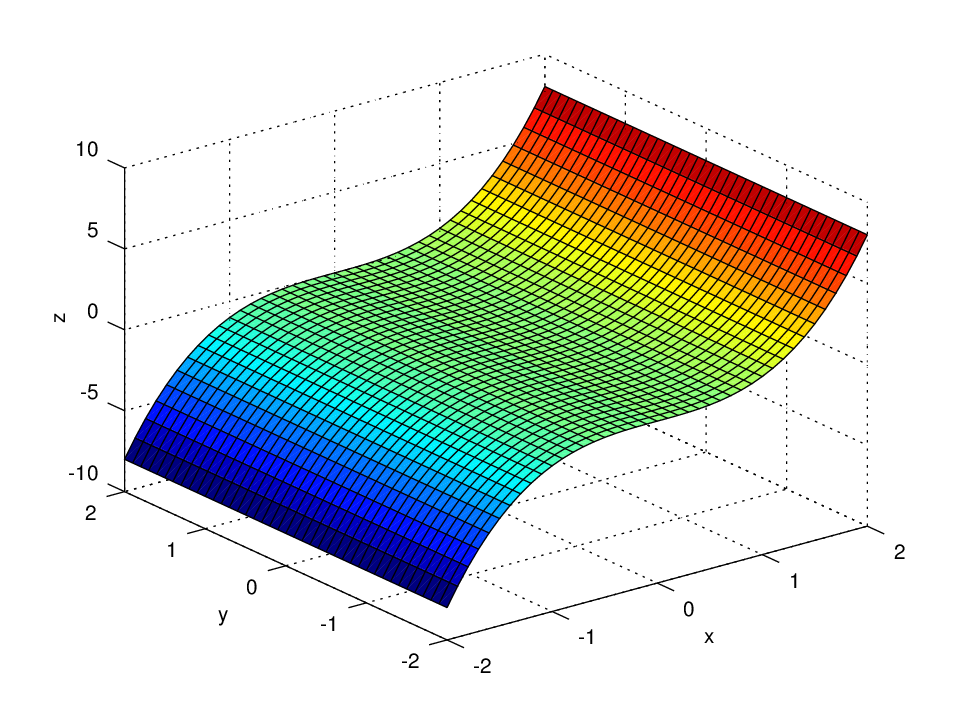
\includegraphics[width=0.600\linewidth]{sodull1.png}\hfill}

\(z = f(x,y) = x^3\).

{\hfill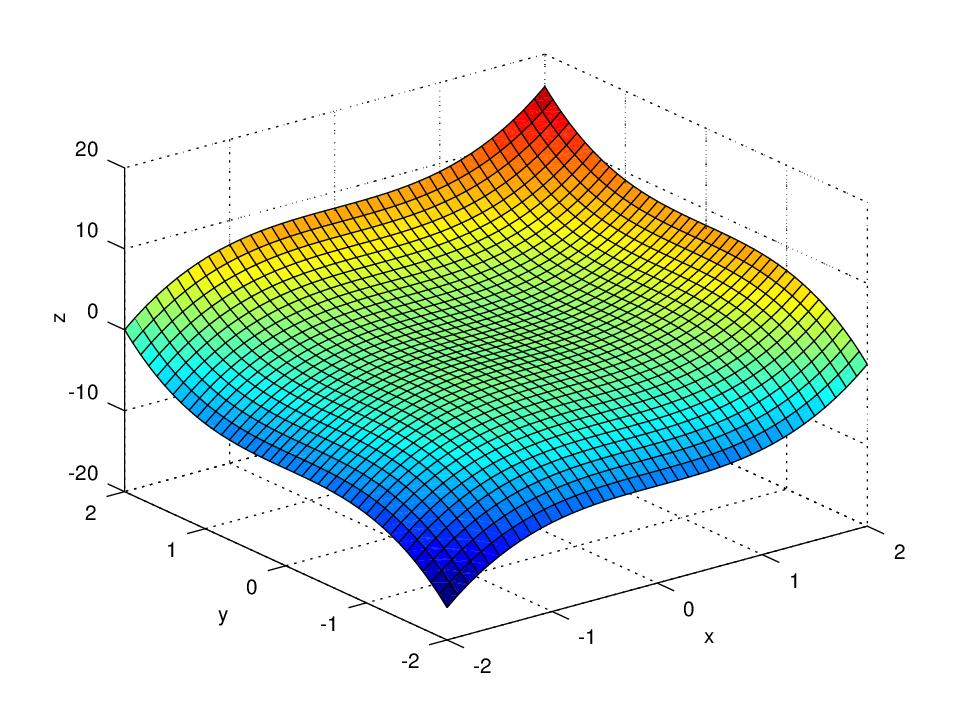
\includegraphics[width=0.600\linewidth]{sodull2.png}\hfill}

\(z = f(x,y) = x^3+y^3\).


\section{Staðbundið útgildi}
\label{Kafli3:id3}

\subsection{Upprifjun}
\label{Kafli3:id4}
Látum \(f\) vera fall af einni breytistærð og gerum ráð fyrir að
\(f'\) sé samfellt fall. Gerum einnig ráð fyrir að \(f'(a)=0\).
Þá gildir:
\begin{enumerate}
\item {} 
Ef \(f''(a)>0\) þá hefur \(f\) \textit{staðbundið lággildi} í
\(a\).

\item {} 
Ef \(f''(a)<0\) þá hefur \(f\) \textit{staðbundið hágildi} í
\(a\).

\item {} 
Ef \(f''(a)=0\) þá gæti verið staðbundið lággildi í \(A\),
það gæti verið staðbundið hágildi í \(a\) eða það gætu verið
beygjuskil í \(a\), alltsvo. ekkert hægt að segja.

\end{enumerate}


\section{Hesse-fylki}
\label{Kafli3:hesse-fylki}

\subsection{Skilgreining}
\label{Kafli3:id5}
Látum \(f\) vera fall af \(n\) breytum
\(\mathbf{x} = (x_1,x_2,\ldots,x_n)\) og gerum ráð fyrir að allar
2. stigs hlutafleiður \(f\) séu skilgreindar í punktinum
\(\mathbf{x}\). Skilgreinum \emph{Hesse-fylki} \(f\) í punktinum
\(\mathbf{x}\) sem \(n\times n\)-fylkið
\begin{gather}
\begin{split}{\cal H}(\mathbf{x})=\begin{bmatrix} f_{11}(\mathbf{x})&f_{12}(\mathbf{x}) & \cdots & f_{1n}(\mathbf{x})\\
 f_{21}(\mathbf{x})&f_{22}(\mathbf{x}) & \cdots & f_{2n}(\mathbf{x}) \\
 \vdots & \vdots & \ddots & \vdots & \\
  f_{n1}(\mathbf{x})&f_{n2}(\mathbf{x}) & \cdots & f_{nn}(\mathbf{x})\end{bmatrix}.\end{split}\notag
\end{gather}
\index{ferningsform}

\section{Ferningsform (sjá kafla 10.7 í Adams)}
\label{Kafli3:index-3}\label{Kafli3:ferningsform-sja-kafla-10-7-i-adams}

\subsection{Upprifjun}
\label{Kafli3:id6}
\textit{Ferningsform} \(Q\) af \(n\)-breytum
\(x_1,x_2,\ldots, x_n\) er einsleit margliða af stigi 2 gefin með
\begin{gather}
\begin{split}Q(\mathbf{x}) = \mathbf{x}^T A \mathbf{x}\end{split}\notag
\end{gather}
þar sem \(A\) er samhverft \(n \times n\) fylki með tölu
\(a_{ij}\) í sæti \((i,j)\) og
\(\mathbf{x} = [x_1,x_2,\ldots x_n]^T\).


\subsection{Skilgreining}
\label{Kafli3:id7}
Ferningsform \(Q\) af \(n\)-breytum er sagt vera \textit{jákvætt ákvarðað} ef \(Q(\mbox{${\bf x}$})>0\) fyrir
alla vigra \(\mbox{${\bf x}$}\neq \mbox{${\bf 0}$}\) í
\(\mbox{${\bf R}^n$}\).

Sagt að ferningsformið \(Q\) sé \textit{neikvætt ákvarðað} ef \(Q(\mbox{${\bf x}$})<0\) fyrir alla vigra
\(\mbox{${\bf x}$}\neq \mbox{${\bf 0}$}\) í
\(\mbox{${\bf R}^n$}\).

Síðan er sagt að ferningsformið \(Q\) sé \textit{óákvarðað}
ef \(Q(\mbox{${\bf x}$})<0\) fyrir einhvern vigur
\(\mbox{${\bf x}$}\) og \(Q(\mbox{${\bf y}$})>0\) fyrir einhvern
vigur \(\mbox{${\bf y}$}\).


\subsection{Setning}
\label{Kafli3:id8}
Látum \(Q\) vera fernings form af \(n\) breytum og \(A\)
samhverft \(n\times n\) fylki þannig að
\(Q(\mbox{${\bf x}$})=\mbox{${\bf x}$}^TA\mbox{${\bf x}$}\) fyrir
alla vigra \(\mbox{${\bf x}$}\),
\begin{enumerate}
\item {} 
Ferningsformið er jákvætt ákvarðað ef og aðeins ef öll \textit{eigingildi}
\(A\) eru jákvæð.

\item {} 
Ferningsformið er neikvætt ákvarðað ef og aðeins ef öll \textit{eigingildi}
\(A\) eru neikvæð.

\item {} 
Ferningsformið er óákvarðað ef og aðeins ef \(A\) hefur bæði
jákvæð og neikvæð \textit{eigingildi}

\end{enumerate}


\section{Staðbundið útgildi}
\label{Kafli3:id9}

\subsection{Setning}
\label{Kafli3:id10}
Látum \(f\) vera fall af \(n\) breytum
\(\mathbf{x} = (x_1,x_2,\ldots,x_n)\) þannig að allar 1. og 2. stigs
hlutafleiður \(f\) eru samfelldar. Látum \(\mathbf{a}\) vera
innri punkt á skilgreiningarsvæði \(f\) og gerum ráð fyrir að
\(\nabla
f(\mathbf{a})=\mbox{${\bf 0}$}\). Þá gildir: Ef
\({\cal H}(\mathbf{a})\) er
\begin{enumerate}
\item {} 
...jákvætt ákvarðað þá hefur \(f\) \textit{staðbundið lággildi} í
\(\mathbf{a}\).

\item {} 
...neikvætt ákvarðað þá hefur \(f\) \textit{staðbundið hágildi} í
\(\mathbf{a}\).

\item {} 
...óákvarðað þá hefur \(f\) \textit{söðulpunkt} í \(\mathbf{a}\).

\item {} 
...hvorki jákvætt ákvarðað, neikvætt ákvarðað né óákvarðað þá nægja
upplýsingarnar sem felast í jöfnunni
\(\nabla f(\mathbf{a})=\mbox{${\bf 0}$}\) og Hesse-fylkinu ekki
til að segja til um hvers eðlis stöðupunkturinn \(\mathbf{a}\)
er.

\end{enumerate}


\subsection{Fylgisetning}
\label{Kafli3:fylgisetning}
Látum \(f\) vera fall af tveim breytum þannig að 1. og 2. stigs
hlutafleiður \(f\) eru samfelldar. Látum \((a,b)\) vera innri
punkt á skilgreiningarsvæði \(f\) og gerum ráð fyrir að
\(\nabla
f(a,b)=\mbox{${\bf 0}$}\). Setjum
\begin{gather}
\begin{split}A=f_{11}(a,b),\qquad\quad B=f_{12}(a,b)=f_{21}(a,b)\qquad\quad
C=f_{22}(a,b).\end{split}\notag
\end{gather}
Þá gildir:
\begin{enumerate}
\item {} 
Ef \(B^2-AC<0\) og \(A>0\) þá hefur \(f\) \textit{staðbundið
lággildi} í \((a,b)\).

\item {} 
Ef \(B^2-AC<0\) og \(A<0\) þá hefur \(f\) \textit{staðbundið
hágildi} í \((a,b)\).

\item {} 
Ef \(B^2-AC>0\) þá hefur \(f\) \textit{söðulpunkt} í \((a,b)\).

\item {} 
Ef \(B^2-AC=0\) þá er ekkert hægt að segja.

\end{enumerate}


\section{Ferningsform}
\label{Kafli3:ferningsform}

\subsection{Regla}
\label{Kafli3:regla}
Ef \(A\) er samhverft \(n \times n\) fylki með tölu
\(a_{ij}\) í sæti \((i,j)\) og
\begin{gather}
\begin{split}D_i = \begin{vmatrix}
        a_{11} & a_{12} & \cdots & a_{1i} \\
        a_{21} & a_{22} & \cdots & a_{2i} \\
        \vdots & \vdots & \ddots & \vdots \\
        a_{i1} & a_{i2} & \cdots & a_{ii}
       \end{vmatrix}\end{split}\notag
\end{gather}
þá gildir
\begin{enumerate}
\item {} 
Ef \(D_i > 0\) fyrir \(1\leq i \leq n\) þá er \(A\)
\textit{jákvætt ákvarðað}.

\item {} 
Ef \(D_i > 0\) fyrir slétt \(i\) í \(\{1,2,\ldots,n\}\)
og \(D_i < 0\) fyrir oddatölu \(i\) í
\(\{1,2,\ldots,n\}\) þá er \(A\) \textit{neikvætt ákvarðað}.

\item {} 
Ef \(\det(A) = D_n \neq 0\) en hvorki \(1\) né \(2\)
gilda þá er \(A\) :hover:\textasciitilde{}óákvarðað,.

\item {} 
Ef \(\det(A) = 0\) þá er \(A\) hvorki jákvætt né neikvætt
ákvarðað en getur verið \textit{óákvarðað}.

\end{enumerate}

\index{skorðujöfnur}

\section{Útgildi falla þar sem breytur uppfylla skorðujöfnur}
\label{Kafli3:index-4}\label{Kafli3:utgildi-falla-ar-sem-breytur-uppfylla-skorujofnur}

\subsection{Sértækar aðferðir}
\label{Kafli3:sertaekar-aferir}
Finna skal útgildi falls \(f(x,y)\) þegar skilgreiningarsvæði
\(f\) er mengi þeirra punkta \((x,y)\) sem uppfylla jöfnu
\(g(x,y)=0\).
\begin{enumerate}
\item {} 
Er mögulegt að einangra \(x\) eða \(y\) í jöfnunni
\(g(x,y)=0\)?
\begin{itemize}
\item {} 
Ef hægt er að einangra \(y\) og rita \(y=h(x)\) þá snýst
verkefnið nú um að finna útgildi falls \(f(x,h(x))\) af einni
breytu \(x\).

\end{itemize}

\item {} 
Er hægt að stika ferilinn \(g(x,y)=0\)?
\begin{itemize}
\item {} 
Ef \(\mbox{${\bf r}$}\) er stikun á ferlinum þá þurfum við að
leita að útgildum fallsins \(f(\mbox{${\bf r}$}(t))\) þar sem
er bara ein breyta.

\end{itemize}

\end{enumerate}


\subsection{Dæmi}
\label{Kafli3:id11}
{\hfill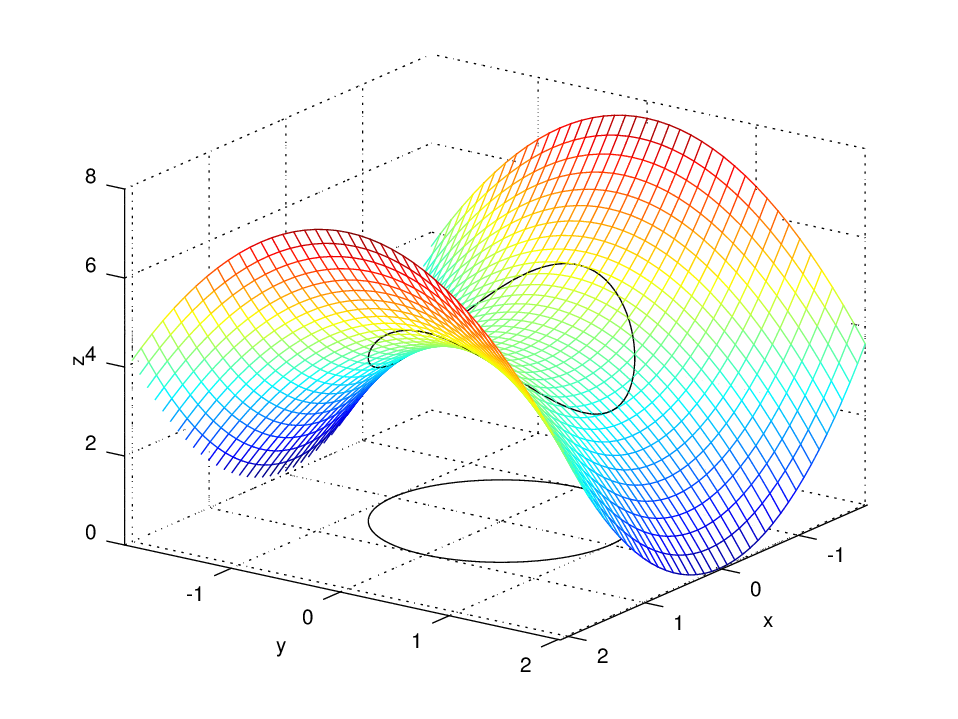
\includegraphics[width=0.600\linewidth]{constraint.png}\hfill}

\emph{Hver eru hæstu og lægstu gildi fallsins} \(f(x,y) = x^2-y^2+4\) \emph{á
menginu} \(\{(x,y)~|~x^2+y^2=1\}\)?


\subsection{Setning}
\label{Kafli3:id12}
Látum \(f\) og \(g\) vera föll sem eru bæði diffranleg í
punktinum \(P_0=(x_0,y_0)\) sem liggur á ferlinum \(g(x,y)=0\),
og er ekki endapunktur ferilsins. Gerum ráð fyrir að
\(\nabla g(x_0,y_0)\neq \mbox{${\bf 0}$}\). Gerum líka ráð fyrir að
ef við einskorðum fallið \(f\) við ferilinn \(g(x,y)=0\) þá hafi
\(f\) staðbundið útgildi í \(P_0\). Þá eru stiglarnir
\(\nabla f(x_0,y_0)\) og \(\nabla g(x_0,y_0)\) samsíða.

{\hfill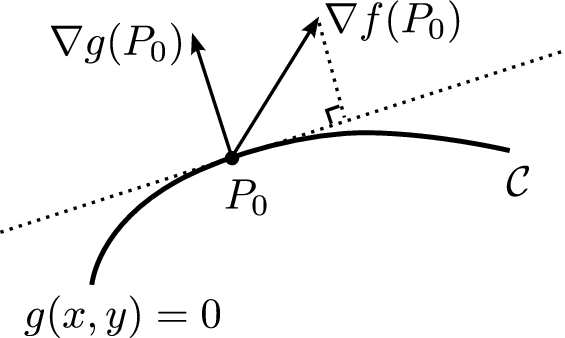
\includegraphics[width=0.400\linewidth]{lagrange1.png}\hfill}

\emph{Ef stiglarnir} \(\nabla g(P_0)\) \emph{og} \(\nabla f(P_0)\) \emph{eru ekki
samsíða þá vex} \(f\) \emph{eða minnkar þegar farið er eftir}
\(\mathcal{C}\) \emph{út frá punktinum} \(P_0\).

\index{Lagrange-margfaldarar}

\section{Lagrange-margfaldarar}
\label{Kafli3:index-5}\label{Kafli3:lagrange-margfaldarar}

\subsection{Reikniaðferð}
\label{Kafli3:reikniafer}
Finna skal útgildi falls \(f(x,y)\) þegar skilgreiningarsvæði
\(f\) er mengi þeirra punkta \((x,y)\) sem uppfylla jöfnu
\(g(x,y)=0\).

Búum til \emph{Lagrange-fallið}
\begin{gather}
\begin{split}L(x,y,\lambda)=f(x,y)+\lambda g(x,y).\end{split}\notag
\end{gather}
\textit{Stöðupunktar} \(L\), þ.e.a.s. punktar \((x_0,y_0,\lambda_0)\) þar
sem \(\nabla L(x_0,y_0,\lambda_0)=\mbox{${\bf 0}$}\), gefa mögulega
punkta \((x_0,y_0)\) þar sem \(f\) tekur útgildi.

Þessir punktar finnast með því að leysa jöfnuhneppið
\begin{gather}
\begin{split}\begin{aligned}
f_1(x,y)+\lambda g_1(x,y)&=0\\
f_2(x,y)+\lambda g_2(x,y)&=0\\
g(x,y)&=0.\end{aligned}\end{split}\notag
\end{gather}
Talan \(\lambda\) nefnist \emph{Lagrange-margfaldari}.


\subsection{Regla}
\label{Kafli3:id13}
Finna skal \textit{útgildi} falls \(f(x,y)\) þegar skilgreiningarsvæði
\(f\) er mengi þeirra punkta \((x,y)\) sem uppfylla jöfnu
\(g(x,y)=0\).

Athuga þarf punkta sem uppfylla eitt af eftirfarandi skilyrðum:
\begin{enumerate}
\item {} 
\textit{Stöðupunktar} \(L(x,y,\lambda)\).

\item {} 
Punktar \((x,y)\) þar sem \(\nabla g(x,y)=\mbox{${\bf 0}$}\)

\item {} 
Punktar \((x,y)\) þar sem annar eða báðir stiglanna
\(\nabla g(x,y)\) og \(\nabla f(x,y)\) eru ekki skilgreindir.

\item {} 
,,Endapunktar” ferilsins \(g(x,y)=0\).

\end{enumerate}


\subsection{Reikniaðferð}
\label{Kafli3:id14}
Finna skal  \textit{útgildi} falls \(f(x,y,z)\) þegar skilgreiningarsvæði
\(f\) er mengi þeirra punkta \((x,y,z)\) sem uppfylla jöfnurnar
\(g(x,y,z)=0\) og \(h(x,y,z)=0\).

Búum til Lagrange-fallið
\begin{gather}
\begin{split}L(x,y,z,\lambda,\mu)=f(x,y,z)+\lambda g(x,y,z)+\mu h(x,y,z).\end{split}\notag
\end{gather}
\textit{Stöðupunktar} \(L\), þ.e.a.s. punktar
\((x_0,y_0,z_0,\lambda_0,\mu_0)\) þar sem
\(\nabla L(x_0,y_0,z_0,\lambda_0,\mu_0)=\mbox{${\bf 0}$}\) gefa
mögulega punkta \((x_0,y_0,z_0)\) þar sem \(f\) tekur  \textit{útgildi}.

Þessir punktar finnast með því að leysa jöfnuhneppið
\begin{gather}
\begin{split}\begin{aligned}
f_1(x,y,z)+\lambda g_1(x,y,z)+\mu h_1(x,y,z)&=0\\
f_2(x,y,z)+\lambda g_2(x,y,z)+\mu h_2(x,y,z)&=0\\
f_3(x,y,z)+\lambda g_3(x,y,z)+\mu h_3(x,y,z)&=0\\
g(x,y,z)&=0\\
h(x,y,z)&=0.\end{aligned}\end{split}\notag
\end{gather}

\chapter{Margföld heildi}
\label{Kafli4::doc}\label{Kafli4:margfold-heildi}
\emph{A bruise is a lesson... and each lesson makes us better.}

- George R.R. Martin, A Game of Thrones

\index{skipting}

\section{Skiptingar}
\label{Kafli4:skiptingar}\label{Kafli4:index-0}

\subsection{Skilgreining}
\label{Kafli4:skilgreining}
Látum \(R=[a,b]\times[c,d]\) vera rétthyrning í planinu. \emph{Skipting}
\(P\) á rétthyrningnum \(R\) felst í því að taka skiptingar
\begin{gather}
\begin{split}\displaystyle\end{split}\notag\\\begin{split}a=x_0<x_1<\cdots<x_m=b\qquad\mbox{og}\qquad
c=y_0<y_1<\cdots<y_n=d\end{split}\notag
\end{gather}
á bilunum \([a,b]\) og \([c,d]\) og nota þær skiptingar til að
skipta \(R\) upp í rétthyrninga
\([x_i,x_{i+1}]\times [y_j,y_{j+1}]\). Ritum
\(\Delta x_i=x_{i+1}-x_i\) og \(\Delta y_j=y_{j+1}-y_j\). \emph{Norm}
skiptingarinnar \(P\), táknað með \(\|P\|\), er skilgreint sem
lengd lengstu hornalínu í rétthyrningunum
\([x_i,x_{i+1}]\times [y_j,y_{j+1}]\).

{\hfill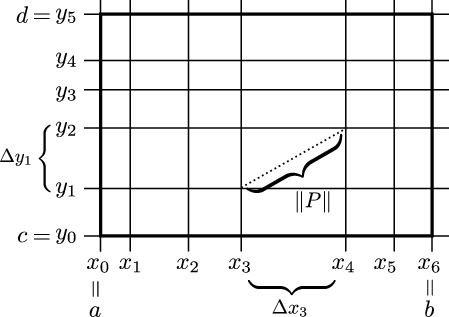
\includegraphics[width=0.500\linewidth]{skipting.png}\hfill}

\emph{Skipting} \(P\) \emph{á rétthyrningi} \(R= [a,b]\times [c,d]\).

\index{Riemann-summa}

\section{Riemann-summa}
\label{Kafli4:riemann-summa}\label{Kafli4:index-1}

\subsection{Skilgreining}
\label{Kafli4:id1}
Látum \(f\) vera fall skilgreint á rétthyrningi
\(R=[a,b]\times[c,d]\) og látum \(P\) vera skiptingu á
\(R\). Veljum úr hverjum rétthyrningi
\([x_i,x_{i+1}]\times [y_j,y_{j+1}]\) punkt \((x_i^*, y_j^*)\).
Skilgreinum \emph{Riemann-summuna}
\begin{gather}
\begin{split}\displaystyle\end{split}\notag\\\begin{split}\mathcal{R}(f,P)=\sum_{i=1}^m\sum_{j=1}^n f(x_i^*, y_j^*)\Delta x_i\Delta
  y_j.\end{split}\notag
\end{gather}
{\hfill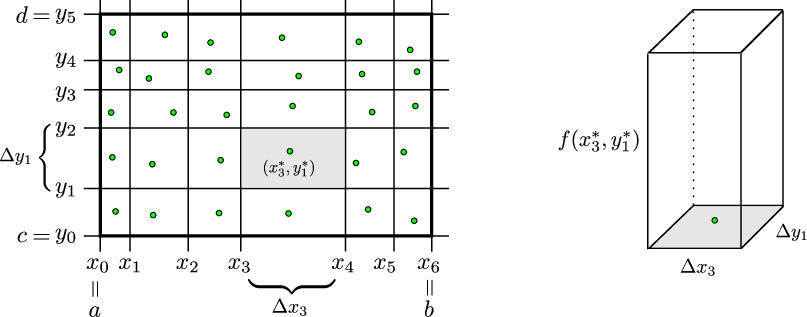
\includegraphics[width=0.800\linewidth]{skipting2.png}\hfill}

{\hfill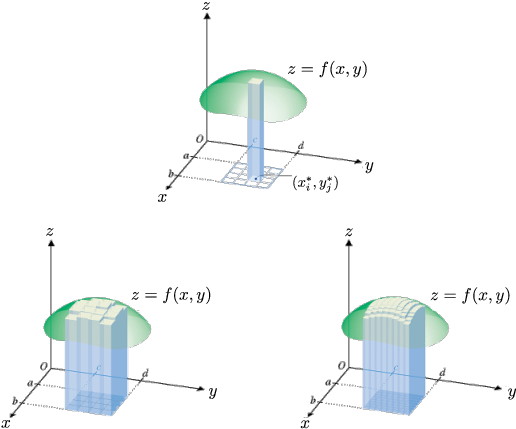
\includegraphics[width=0.750\linewidth]{double.png}\hfill}

\index{heildi!tvöfalt heildi}

\section{Tvöfalt heildi yfir rétthyrning}
\label{Kafli4:tvofalt-heildi-yfir-retthyrning}\label{Kafli4:index-2}

\subsection{Skilgreining}
\label{Kafli4:id2}
Sagt er að fall \(f\) skilgreint á rétthyrningi
\(R=[a,b]\times [c,d]\) sé \textit{heildanlegt} yfir \(R\) með \textit{heildi}
\(I\) (hér stendur \(I\) fyrir tölu) ef fyrir sérhvert
\(\varepsilon>0\) er til tala \(\delta>0\) þannig að
\(|\mathcal{R}(f,P)-I|<\varepsilon\) fyrir allar skiptingar
\(P\) með \(\|P\|<\delta\) óháð vali á punktunum
\((x_i^*, y_j^*)\).

Ritum þá
\begin{gather}
\begin{split}\displaystyle \int\!\!\!\int_R f(x,y)dA=I.\end{split}\notag
\end{gather}

\section{Tvöfalt heildi yfir takmarkað svæði}
\label{Kafli4:tvofalt-heildi-yfir-takmarka-svaei}

\subsection{Skilgreining}
\label{Kafli4:id3}
Látum \(D\) vera takmarkað svæði í planinu. Fall \(f\) er sagt
\textit{heildanlegt} yfir \(D\) ef til er rétthyrningur \(R\) sem
inniheldur \(D\) og fallið
\begin{gather}
\begin{split}\displaystyle\end{split}\notag\\\begin{split}\hat{f}(x,y)=\left\{\begin{array}{rcl}
f(x,y)& & \mbox{ef }(x,y)\in D,\\
0& & \mbox{ef }(x,y)\in R\setminus D
\end{array}\right.\end{split}\notag
\end{gather}
er heildanlegt yfir \(R\).


\subsection{Setning}
\label{Kafli4:setning}
Látum \(f\) vera samfellt fall skilgreint á lokuðu og takmörkuðu
svæði \(D\) í planinu \({\mathbb  R}^2\). Gerum ráð fyrir að
jaðar \(D\) samanstandi af endanlega mörgum ferlum sem hafa
endanlega lengd. Þá er fallið \(f\) \textit{heildanlegt} yfir \(D\).


\subsection{Setning}
\label{Kafli4:id4}
Látum \(D\) vera svæði í planinu og \(f\) \textit{takmarkað} fall
skilgreint á \(D\) og \textit{heildanlegt} yfir \(D\). Þá gildir:
\begin{enumerate}
\item {} 
\(\int\!\!\!\int_D f(x,y)\,dA=0\) ef flatarmál \(D\) er 0.

\item {} 
\(\int\!\!\!\int_D 1\,dA=\) flatarmál \(D\).

\item {} 
Ef \(f(x,y)\geq 0\) fyrir alla punkta \((x,y)\) í \(D\)
þá er \(\int\!\!\!\int_D f(x,y)\,dA\) jafnt rúmmáli rúmskikans
sem liggur milli \(D\) og grafsins \(z=f(x,y)\).

\item {} 
Ef \(f(x,y)\leq 0\) fyrir alla punkta \((x,y)\) í \(D\)
þá er \(\int\!\!\!\int_D f(x,y)\,dA\) jafnt mínus rúmmáli
rúmskikans sem liggur milli \(D\) og grafsins \(z=f(x,y)\).

\end{enumerate}


\subsection{Setning}
\label{Kafli4:id5}
Ef \(D\) er svæði í planinu og \(f\) og \(g\) heildanleg
föll yfir \(D\) þá gildir:
\begin{enumerate}
\item {} 
Ef \(L\) og \(M\) eru fastar þá er
\begin{gather}
\begin{split}\displaystyle\end{split}\notag\\\begin{split}\int\!\!\!\int_D Lf(x,y)+Mg(x,y)\,dA=L\!\int\!\!\!\int_D f(x,y)\,dA+M\!\int\!\!\!\int_D
g(x,y)\,dA.\end{split}\notag
\end{gather}
\item {} 
Ef \(f(x,y)\leq g(x,y)\) þá er
\begin{gather}
\begin{split}\displaystyle \int\!\!\!\int_D f(x,y)\,dA\leq \int\!\!\!\int_Dg(x,y)\,dA.\end{split}\notag
\end{gather}
\item {} 
Þríhyrningsójafna:

\end{enumerate}
\begin{quote}
\begin{gather}
\begin{split}\bigg|\int\!\!\!\int_D f(x,y)\,dA\bigg|\leq \int\!\!\!\int_D |f(x,y)|\,dA.\end{split}\notag
\end{gather}\end{quote}
\begin{enumerate}
\item {} 
Ritum \(D\) sem sammengi af svæðum \(D_1,\ldots, D_k\) sem
skarast ekki nema mögulega í jaðarpunktum þá er
\begin{gather}
\begin{split}\displaystyle \int\!\!\!\int_D f(x,y)\,dA=\sum_{i=1}^k\int\!\!\!\int_{D_i}f(x,y)\,dA.\end{split}\notag
\end{gather}
\end{enumerate}

\index{Fubini!setning Fubinis}

\subsection{Setning Fubinis}
\label{Kafli4:setning-fubinis}\label{Kafli4:index-3}
Látum \(f\) vera fall sem er \textit{samfellt} á rétthyrningi
\(R=[a,b]\times
[c,d]\). Setjum
\begin{gather}
\begin{split}\displaystyle A(x)=\int_c^d f(x,y)\,dy\qquad\mbox{($x$ hugsað sem fasti þegar heildað)}.\end{split}\notag
\end{gather}
Þá gildir að
\begin{gather}
\begin{split}\displaystyle\end{split}\notag\\\begin{split}\int\!\!\!\int_R f(x,y)\,dA=\int_a^b A(x)\,dx=\int_a^b\!\!\int_c^d
f(x,y)\,dy\,dx.\end{split}\notag
\end{gather}
Sömuleiðis gildir þegar við setjum
\begin{gather}
\begin{split}\displaystyle A(y)=\int_a^b f(x,y)\,dx\qquad\mbox{($y$ hugsað sem fasti þegar heildað)} \qquad \text{að}\end{split}\notag
\end{gather}\begin{gather}
\begin{split}\displaystyle\end{split}\notag\\\begin{split}\int\!\!\!\int_R f(x,y)\,dA=\int_c^d A(y)\,dy=\int_c^d\!\!\int_a^b
f(x,y)\,dx\,dy.\end{split}\notag
\end{gather}
{\hfill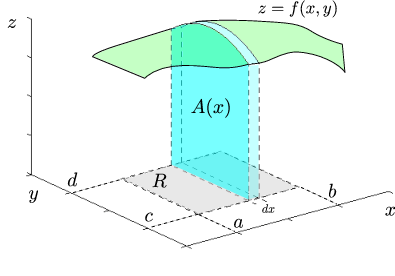
\includegraphics[width=0.500\linewidth]{ax1.png}\hfill}


\section{\(x\)-einföld og \(y\)-einföld svæði}
\label{Kafli4:einfold-og-einfold-svaei}
\index{x-einfaldur}\index{y-einfaldur}

\subsection{Skilgreining}
\label{Kafli4:index-4}\label{Kafli4:id6}
Svæði \(D\) í planinu er sagt vera \(y\)\emph{-einfalt} ef hægt er
að finna tölur \(a\) og \(b\) og föll \(c(x)\) og
\(d(x)\) þannig að
\begin{gather}
\begin{split}\displaystyle D=\{(x,y)\mid a\leq x\leq b, c(x)\leq y\leq d(x)\}.\end{split}\notag
\end{gather}
Svæði \(D\) í planinu er sagt vera \(x\)\emph{-einfalt} ef hægt er
að finna tölur \(c\) og \(d\) og föll \(a(y)\) og
\(b(y)\) þannig að
\begin{gather}
\begin{split}\displaystyle D=\{(x,y)\mid c\leq y\leq d, a(y)\leq x\leq b(y)\}.\end{split}\notag
\end{gather}
{\hfill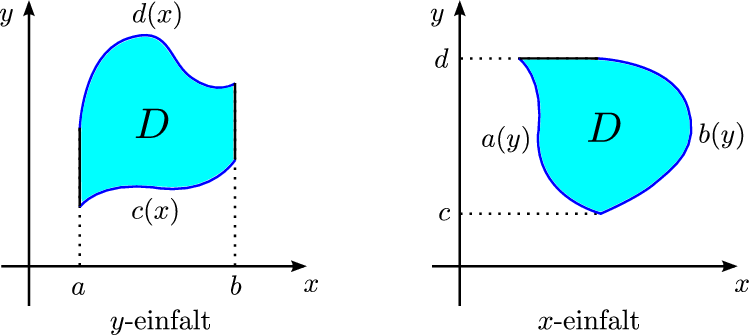
\includegraphics[width=0.650\linewidth]{einfalt.png}\hfill}


\subsection{Regla}
\label{Kafli4:regla}
Lokað og takmarkað svæði \(D\) í planinu er \(y\)-einfalt ef og
aðeins ef sérhver lína af gerðinni \(x=x_0\) sker \(D\) í
línustriki.

Lokað og takmarkað svæði \(D\) er \(x\)-einfalt ef og aðeins ef
sérhver lína af gerðinni \(y=y_0\) sker svæðið í línustriki.


\section{Heildi yfir \(x\)-einföld og \(y\)-einföld svæði}
\label{Kafli4:heildi-yfir-einfold-og-einfold-svaei}

\subsection{Setning}
\label{Kafli4:id7}
Látum \(D=\{(x,y)\mid a\leq x\leq b, c(x)\leq y\leq d(x)\}\) vera
\(y\)-einfalt svæði og \(f(x,y)\) fall sem er heildanlegt yfir
\(D\). Þá er
\begin{gather}
\begin{split}\displaystyle \int\!\!\!\int_D f(x,y)\,dA=\int_a^b\!\!\!\int_{c(x)}^{d(x)}f(x,y)\,dy\, dx.\end{split}\notag
\end{gather}
Látum \(D=\{(x,y)\mid c\leq y\leq d, a(y)\leq x\leq b(y)\}\) vera
\(x\)-einfalt svæði og \(f(x,y)\) fall sem er heildanlegt yfir
\(D\). Þá er
\begin{gather}
\begin{split}\displaystyle \int\!\!\!\int_D f(x,y)\,dA=\int_c^d\!\!\!\int_{a(y)}^{b(y)}f(x,y)\,dx\, dy.\end{split}\notag
\end{gather}
{\hfill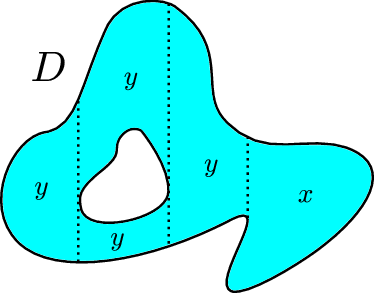
\includegraphics[width=0.350\linewidth]{einfalt2.png}\hfill}

\emph{Hér er svæðinu} \(D\) \emph{skipt í endanlega mörg} \(x\)-\emph{einföld} og \(y\)-\emph{einföld svæði sem skarast eingöngu í punktum á jaðrinum.}

\index{heildi!óeiginlegt heildi}

\section{Óeiginleg heildi}
\label{Kafli4:index-5}\label{Kafli4:oeiginleg-heildi}

\subsection{Umræða}
\label{Kafli4:umraea}
Látum \(f(x,y)\geq 0\) vera jákvætt fall sem er skilgreint á svæði
\(D\) í sléttunni. Ef
\begin{enumerate}
\item {} 
\(D\) er ótakmarkað svæði eða

\item {} 
\(f(x,y)\) er ótakmarkað á \(D\)

\end{enumerate}

má í sumum tilfellum skilgreina tvöfalda heildið af \(f\) yfir
\(D\).

Það er gert með því að finna fyrst runu af stækkandi lokuðum og
takmörkuðum mengjum
\(D_1 \subseteq D_2 \subseteq \cdots \subseteq D\) sem ’stefnir á’
\(D\). Ef
\begin{gather}
\begin{split}\displaystyle \int\!\!\!\int_{D_n} f(x,y)\,dA\end{split}\notag
\end{gather}
er vel skilgreint fyrir öll \(n\) og hefur markgildi þegar
\(n\to \infty\) (fyrir allar ólíkar runur \((D_n)_{n\geq 1}\))
þá skilgreinum við \textit{óeiginlega heildið}
\begin{gather}
\begin{split}\displaystyle \int\!\!\!\int_{D} f(x,y)\,dA := \lim_{n\to \infty} \int\!\!\!\int_{D_n} f(x,y)\,dA .\end{split}\notag
\end{gather}

\subsection{Skilgreining}
\label{Kafli4:id8}
Látum \(f\) vera fall sem er heildanlegt yfir svæði \(D\) í
\({\mathbb  R}^2\). \emph{Meðalgildi} fallsins \(f\) á \(D\) er
skilgreint sem talan
\begin{gather}
\begin{split}\displaystyle \bar{f}=\frac{1}{\mbox{flatarmál }D}\int\!\!\!\int_D f(x,y)\,dA.\end{split}\notag
\end{gather}
\index{samanhangandi}\index{ferilsamanhangandi}

\subsection{Skilgreining}
\label{Kafli4:id9}\label{Kafli4:index-6}
Segjum að mengi \(D\subseteq {\mathbb  R}^2\) sé
\emph{ferilsamanhangandi} (e. path-connected) ef fyrir sérhverja
tvo punkta \(P, Q\in D\) gildir að til er stikaferill
\(\mbox{${\bf r}$}:[0,1]\rightarrow D\) þannig að
\(\mbox{${\bf r}$}(0)=P\) og \(\mbox{${\bf r}$}(1)=Q\).

\begin{notice}{warning}{Aðvörun:}
Í bók er orðið \emph{connected} notað fyrir hugtakið \emph{ferilsamanhangandi}. Venjulega er orðið \emph{connected} notað yfir annað hugtak, skylt en samt ólíkt.
\end{notice}

\index{meðalgildissetning}

\subsection{Setning (\textit{Meðalgildissetning} fyrir tvöföld heildi)}
\label{Kafli4:index-7}\label{Kafli4:setning-fyrir-tvofold-heildi}
Gerum ráð fyrir að \(f\)
sé samfellt fall sem er skilgreint á lokuðu, takmörkuðu og ferilsamanhangandi
svæði \(D\) í \({\mathbb  R}^2\). Þá er til punktur
\((x_0,y_0)\) í \(D\) þannig að
\begin{gather}
\begin{split}\displaystyle \frac{1}{\mbox{flatarmál }D}\int\!\!\!\int_D f(x,y)\,dA=f(x_0,y_0).\end{split}\notag
\end{gather}
\index{breytuskipti}

\section{Breytuskipti}
\label{Kafli4:index-8}\label{Kafli4:breytuskipti}

\subsection{Upprifjun}
\label{Kafli4:upprifjun}
Látum \(P=(x,y)\neq \mbox{${\bf 0}$}\) vera punkt í plani. \textit{Pólhnit}
\(P\) er talnapar \([r,\theta]\) þannig að \(r\) er fjarlægð
\(P\) frá \(O=(0,0)\) og \(\theta\) er hornið á milli
striksins \(\overline{OP}\) og \(x\)-ássins. (Hornið er mælt
þannig að rangsælis stefna telst jákvæð, og leggja má við \(\theta\)
heil margfeldi af \(2\pi\).)

\index{pólhnitarétthyrningur}

\subsection{Skilgreining}
\label{Kafli4:id10}\label{Kafli4:index-9}
\emph{Pólhnitarétthyrningur} í \(xy\)-planinu er svæði sem afmarkast af
tveimur hringbogum \(x^2+y^2=a^2\) og \(x^2+y^2=b^2\) og tveimur
hálflínum sem byrja í \((0,0)\) og mynda hornin \(\alpha\) og
\(\beta\) við \(x\)-ásinn (Hornin eru mæld þannig að rangsælis
stefna telst jákvæð.)

{\hfill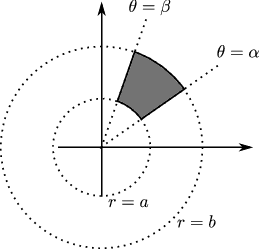
\includegraphics[width=0.400\linewidth]{polarrett.png}\hfill}

Gerum ráð fyrir að \(0\leq a\leq b\) og að
\(0\leq\beta-\alpha\leq
2\pi\). Þá má lýsa pólhnitarétthyrningnum með því að nota pólhnit þannig
að
\begin{gather}
\begin{split}\displaystyle D=\{[r,\theta]\mid 0\leq a\leq r\leq b, \alpha\leq \theta\leq\beta\}.\end{split}\notag
\end{gather}

\subsection{Setning}
\label{Kafli4:id11}
Ef \(f\) er fall sem er \textit{heildanlegt} yfir pólhnitarétthyrning
\(D=\{[r,\theta]\mid 0\leq a\leq r\leq b, \alpha\leq \theta\leq\beta\}\)
þá er
\begin{gather}
\begin{split}\displaystyle\end{split}\notag\\\begin{split}\int\!\!\!\int_D f(x,y)\,dA=\int_\alpha^\beta\!\!\!\int_{a}^{b}
f(r\cos\theta,r\sin\theta)\,r\,dr\, d\theta.\end{split}\notag
\end{gather}
{\hfill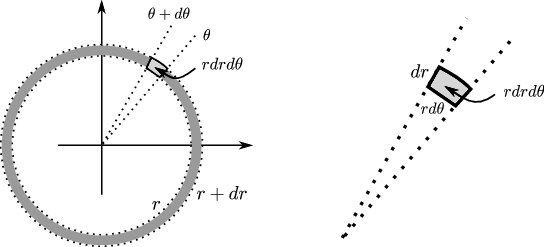
\includegraphics[width=0.900\linewidth]{polarelement.png}\hfill}

\index{pólhnitagraf}

\subsection{Upprifjun}
\label{Kafli4:id12}\label{Kafli4:index-10}
Látum \(f\) vera fall skilgreint á bili \([\alpha,\beta]\).
Jafnan \(r=f(\theta)\) lýsir mengi allra punkta í planinu sem hafa
\textit{pólhnit} á forminu \([f(\theta),\theta]\) þar sem
\(\alpha\leq\theta\leq\beta\). Þetta mengi kallast \emph{pólhnitagraf}
fallsins \(f\).


\subsection{Setning}
\label{Kafli4:id13}
Látum \(D\) vera svæði í \(xy\)-plani sem afmarkast af
pólhnitalínum \(\theta=\alpha\) og \(\theta=\beta\) og tveimur
pólhnitagröfum \(r=a(\theta)\) og \(r=b(\theta)\). Gerum ráð
fyrir að \(0\leq a(\theta)\leq
r\leq b(\theta)\) og \(0\leq \beta-\alpha\leq 2\pi\). Ef \(f\) er
heildanlegt fall yfir \(D\) þá er
\begin{gather}
\begin{split}\displaystyle\end{split}\notag\\\begin{split}\int\!\!\!\int_D\,f(x,y)\,dA=\int_\alpha^\beta\!\!\!\int_{a(\theta)}^{b(\theta)}
f(r\cos\theta,r\sin\theta)\,r\,dr\, d\theta.\end{split}\notag
\end{gather}
{\hfill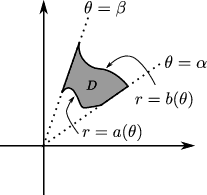
\includegraphics[width=0.450\linewidth]{polarsvaedi.png}\hfill}


\subsection{Regla}
\label{Kafli4:id14}
Hugsum okkur að \(f(x,y)\) sé fall og hægt sé að rita
\(f(x,y)=g(x)h(y)\). Látum \(R=[a,b]\times [c,d]\). Þá er
\begin{gather}
\begin{split}\displaystyle\end{split}\notag\\\begin{split}\begin{aligned}
\int\!\!\!\int_R f(x,y)\,dA&=\int_a^b\!\!\!\int_{c}^{d}g(x)h(y)\,dy\, dx\\
&=\bigg(\int_a^b g(x)\,dx\bigg)\bigg(\int_c^d h(y)\,dy\bigg).\end{aligned}\end{split}\notag
\end{gather}

\subsection{Setning (Almenn breytuskiptaregla fyrir tvöföld heildi)}
\label{Kafli4:setning-almenn-breytuskiptaregla-fyrir-tvofold-heildi}
Látum \(x=x(u,v)\), \(y=y(u,v)\) vera gagntæka vörpun milli
svæðis \(S\) í \(uv\)-plani og svæðis \(D\) í
\(xy\)-plani. Gerum ráð fyrir að föllin \(x(u,v)\),
\(y(u,v)\) hafi samfelldar fyrsta stigs hlutafleiður á \(S\). Ef
\(f\) er heildanlegt fall yfir \(D\), þá er fallið
\(g(u,v)=f(x(u,v), y(u,v))\) heildanlegt yfir \(S\) og
\begin{gather}
\begin{split}\displaystyle\end{split}\notag\\\begin{split}\int\!\!\!\int_D f(x,y)\,dx\,dy=\int\!\!\!\int_S g(u,v)
\bigg|\frac{\partial(x,y)}{\partial(u,v)}\bigg|\,du\,dv.\end{split}\notag
\end{gather}
{\hfill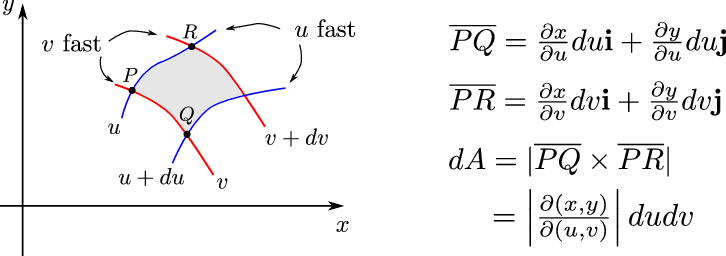
\includegraphics[width=0.900\linewidth]{changevar.png}\hfill}

\index{heildi!þrefalt heildi}

\section{Þreföld heildi}
\label{Kafli4:refold-heildi}\label{Kafli4:index-11}

\subsection{Umræða}
\label{Kafli4:id15}
\textit{Heildi} falls \(f(x,y,z)\) yfir kassa
\(K=[a,b]\times[c,d]\times[u,v]\) í \({\mathbb  R}^3\) er
skilgreint á sambærilegan hátt og tvöfalt heildi er skilgreint.

Á sama hátt og fyrir tvöföld heildi má svo skilgreina heildi fyrir
almennari \textit{rúmskika}.

\textit{Heildi} falls \(f(x,y,z)\) yfir \textit{rúmskika} \(R\) er táknað með
\begin{gather}
\begin{split}\displaystyle \int\!\!\!\int\!\!\!\int_R f(x,y,z)\,dV.\end{split}\notag
\end{gather}
(\(dV\) stendur fyrir að heildað er með tilliti til rúmmáls.)


\subsection{Setning}
\label{Kafli4:id16}
Látum \(f(x,y,z)\) vera fall sem er \textit{heildanlegt} yfir kassa
\(K=[a,b]\times[c,d]\times[u,v]\) í \({\mathbb  R}^3\). Þá er
\begin{gather}
\begin{split}\displaystyle\end{split}\notag\\\begin{split}\int\!\!\!\int\!\!\!\int_K f(x,y,z)\,dV=
\int_a^b\!\int_c^d\!\int_u^v f(x,y,z)\,dz\,dy\,dx.\end{split}\notag
\end{gather}
Breyta má röð heilda að vild, t.d. er
\begin{gather}
\begin{split}\displaystyle\end{split}\notag\\\begin{split}\int\!\!\!\int\!\!\!\int_K f(x,y,z)\,dV=
\int_u^v\!\int_c^d\!\int_a^b f(x,y,z)\,dx\,dy\,dz.\end{split}\notag
\end{gather}

\subsection{Setning}
\label{Kafli4:id17}
Látum \(f(x,y,z)\) vera fall sem er heildanlegt yfir rúmskika
\(R\) og gerum ráð fyrir að \(R\) hafi lýsingu á forminu
\begin{gather}
\begin{split}\displaystyle R=\{(x,y,z)\mid a\leq x\leq b,\ c(x)\leq y\leq d(x),\ u(x,y)\leq z\leq v(x,y)\}.\end{split}\notag
\end{gather}
Þá er
\begin{gather}
\begin{split}\displaystyle\end{split}\notag\\\begin{split}\int\!\!\!\int\!\!\!\int_R f(x,y,z)\,dV=
\int_a^b\!\int_{c(x)}^{d(x)}\!\int_{u(x,y)}^{v(x,y)} f(x,y,z)\,dz\,dy\,dx.\end{split}\notag
\end{gather}
Breyturnar \(x, y, z\) geta svo skipt um hlutverk.


\subsection{Setning (Almenn breytuskiptaformúla fyrir þreföld heildi.)}
\label{Kafli4:setning-almenn-breytuskiptaformula-fyrir-refold-heildi}
Látum
\begin{gather}
\begin{split}\displaystyle (u,v,w)\mapsto (x(u,v,w), y(u,v,w), z(u,v,w))\end{split}\notag
\end{gather}
vera gagntæka vörpun milli rúmskika \(R\) í \(xyz\)-rúmi og
rúmskika \(S\) í \(uvw\)-rúmi. Gerum ráð fyrir að föllin
\(x(u,v,w), y(u,v,w), z(u,v,w)\) hafi öll samfelldar fyrsta stigs
hlutafleiður. Ef \(f(x,y,z)\) er fall sem er heildanlegt yfir
\(R\) þá er
\begin{gather}
\begin{split}\displaystyle\end{split}\notag\\\begin{split}\begin{aligned}
\int\!\!\!\int\!\!\!\int_R& f(x,y,z)\,dV \\&=\int\!\!\!\int\!\!\!\int_S f(x(u,v,w), y(u,v,w), z(u,v,w))
\bigg|\frac{\partial(x,y,z)}{\partial(u,v,w)}\bigg|\,du\,dv\,dw.\end{aligned}\end{split}\notag
\end{gather}
\index{sívalningshnit}

\subsection{Skilgreining}
\label{Kafli4:index-12}\label{Kafli4:id18}
Látum \((x,y,z)\) vera punkt í \({\mathbb  R}^3\).
\textit{Sívalningshnit} \((x,y,z)\) eru þrennd talna \(r, \theta, z\)
þannig að
\begin{gather}
\begin{split}\displaystyle x=r\cos\theta\qquad\qquad y=r\sin\theta\qquad\qquad z=z.\end{split}\notag
\end{gather}
\begin{notice}{note}{Athugasemd:}
Athugið að \([r,\theta]\) eru pólhnit punktsins \((x,y)\).
\end{notice}

\index{sívalningshnit!breytuskipti}

\subsection{Setning (Breytuskipti yfir í sívalningshnit.)}
\label{Kafli4:index-13}\label{Kafli4:setning-breytuskipti-yfir-i-sivalningshnit}
Látum \(R\) vera rúmskika í \({\mathbb  R}^3\) og látum
\(f(x,y,z)\) vera heildanlegt fall yfir \(R\). Gerum ráð fyrir
að \(R\) megi lýsa með eftirfarandi skorðum á sívalningshnit
punktanna sem eru í \(R\)
\begin{gather}
\begin{split}\displaystyle \alpha\leq \theta\leq \beta,\ a(\theta)\leq r\leq  b(\theta), u(r,\theta)\leq z\leq v(r,\theta),\end{split}\notag
\end{gather}
þar sem \(0\leq \beta-\alpha\leq 2\pi\). Þá er
\begin{gather}
\begin{split}\displaystyle\end{split}\notag\\\begin{split}\int\!\!\!\int\!\!\!\int_R f(x,y,z)\,dV=
\int_\alpha^\beta
\!\int_{a(\theta)}^{b(\theta)}\int_{u(r,\theta)}^{v(r,\theta)}
f(r\cos\theta,r\sin\theta,z)r\,dz\,dr\,d\theta.\end{split}\notag
\end{gather}
\index{kúluhnit}

\section{Kúluhnit}
\label{Kafli4:index-14}\label{Kafli4:kuluhnit}

\subsection{Skilgreining}
\label{Kafli4:id19}
Látum \((x,y,z)\) vera punkt í \({\mathbb  R}^3\). \textit{Kúluhnit}
\((x,y,z)\) eru þrennd talna \(\rho, \varphi, \theta\) þannig að
\begin{gather}
\begin{split}\displaystyle x=\rho\sin\varphi\cos\theta\qquad\qquad y=\rho\sin\varphi\sin\theta\qquad\qquad z=\rho\cos\varphi.\end{split}\notag
\end{gather}
Punktur sem hefur kúluhnit \(\rho, \varphi, \theta\) er táknaður með
\([\rho, \varphi, \theta]\).

{\hfill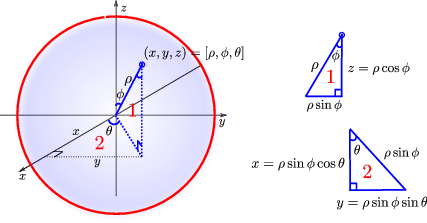
\includegraphics[width=0.800\linewidth]{sphere.png}\hfill}


\subsection{Umræða}
\label{Kafli4:id20}
Eftirfarandi jöfnur gefa aðferð til að finna \textit{kúluhnit}:
\begin{itemize}
\item {} 
\(\rho\) er fjarlægðin frá \((0,0,0)\) til \((x,y,z)\), það er að
segja
\begin{gather}
\begin{split}\displaystyle \rho=\sqrt{x^2+y^2+z^2}.\end{split}\notag
\end{gather}
\item {} 
\(\varphi\) er hornið á milli jákvæða hluta \(z\)-ássins og línustriksins frá
\((0,0,0)\) til \((x,y,z)\). Hornið \(\varphi\) má
ákvarða út frá jöfnunni
\begin{gather}
\begin{split}\displaystyle \tan\varphi=\frac{\sqrt{x^2+y^2}}{z}.\end{split}\notag
\end{gather}
\item {} 
\(\theta\) er hornið sem jákvæði hluti \(x\)-ásins myndar við línustrikið
frá \((0,0,0)\) til \((x,y,0)\) (sama horn og notað í
sívalningshnitum (og pólhnitum)). Hornið \(\theta\) má finna út
frá jöfnunni
\begin{gather}
\begin{split}\displaystyle \tan\theta=\frac{y}{x}.\end{split}\notag
\end{gather}
\end{itemize}

Um kúluhnit \([\rho, \varphi, \theta]\) fyrir punkt \((x,y,z)\)
gildir að velja má \(\rho, \varphi, \theta\) þannig að
\(0\leq \rho\), \(0\leq\varphi\leq \pi\) og
\(0\leq\theta\leq 2\pi\).

\index{kúluhnit!breytuskipti}

\section{Breytuskipti í kúluhnit}
\label{Kafli4:breytuskipti-i-kuluhnit}\label{Kafli4:index-15}

\subsection{Setning}
\label{Kafli4:id21}
Látum \(R\) vera rúmskika þannig að þegar notuð eru \textit{kúluhnit} þá fæst
eftirfarandi lýsing
\begin{gather}
\begin{split}\displaystyle\end{split}\notag\\\begin{split}R=\{[\rho,\varphi,\theta]\mid \alpha\leq\theta\leq\beta,
c\leq\varphi\leq d, a\leq \rho\leq b\}.\end{split}\notag
\end{gather}
Ef \(f\) er fall sem er \textit{heildanlegt} yfir \(R\) þá er
\begin{gather}
\begin{split}\displaystyle\end{split}\notag\\\begin{split}\begin{aligned}
&\int\!\!\!\int\!\!\!\int_R f(x,y,z)\,dV=\\ &\int_\alpha^\beta\!\int_c^d\!\int_a^b f(\rho\sin\varphi\cos\theta, \rho\sin\varphi\sin\theta,\rho\cos\varphi)
\,\rho^2\sin\varphi\,d\rho\,d\varphi\,d\theta.\end{aligned}\end{split}\notag
\end{gather}
\index{massamiðja}\index{vægi}

\section{Massamiðja}
\label{Kafli4:index-16}\label{Kafli4:massamija}

\subsection{Regla}
\label{Kafli4:id22}
Látum \(D\) tákna svæði í plani. Hugsum \(D\) sem plötu þ.a. í
punkti \((x,y)\) er efnisþéttleikinn gefinn með falli
\(\delta(x,y)\). Massi plötunnar er
\begin{gather}
\begin{split}\displaystyle m=\int\!\!\!\int_D \delta(x,y)\,dA.\end{split}\notag
\end{gather}
\emph{Vægi} plötunnar um línuna \(x=0\) (þ.e. \(y\)-ás) og um línuna
\(y=0\) (þ.e. \(x\)-ás) eru gefin með
\begin{gather}
\begin{split}\displaystyle M_{x=0}=\int\!\!\!\int_D x\delta(x,y)\,dA \quad \text{og} \quad M_{y=0}=\int\!\!\!\int_D y\delta(x,y)\,dA.\end{split}\notag
\end{gather}
Hnit \emph{massamiðju} plötunnar eru \((\overline{x}, \overline{y})\) þar
sem
\begin{gather}
\begin{split}\displaystyle \overline{x}=\frac{M_{x=0}}{m} \quad \text{og}\quad \overline{y}=\frac{M_{y=0}}{m}.\end{split}\notag
\end{gather}

\subsection{Regla}
\label{Kafli4:id23}
Látum \(R\) tákna \textit{rúmskika}. Hugsum \(R\) sem hlut þannig að í
punkti \((x,y,z)\) er efnisþéttleikinn gefinn með falli
\(\delta(x,y,z)\). Massi hlutarins er
\begin{gather}
\begin{split}\displaystyle m=\int\!\!\!\int\!\!\!\int_R \delta(x,y,z)\,dV.\end{split}\notag
\end{gather}
\emph{Vægi} hlutarins um planið \(x=0\) (þ.e. \(yz\)-planið) er
\begin{gather}
\begin{split}\displaystyle M_{x=0}=\int\!\!\!\int\!\!\!\int_R x\delta(x,y,z)\,dV.\end{split}\notag
\end{gather}
Svipað skilgreinum við
\begin{gather}
\begin{split}\displaystyle M_{y=0}=\int\!\!\!\int\!\!\!\int_R y\delta(x,y,z)\,dV \quad \text{og}\quad M_{z=0}=\int\!\!\!\int\!\!\!\int_R z\delta(x,y,z)\,dV.\end{split}\notag
\end{gather}
Hnit \emph{massamiðju} hlutarins eru
\((\overline{x}, \overline{y}, \overline{z})\) þar sem
\begin{gather}
\begin{split}\displaystyle\end{split}\notag\\\begin{split}\overline{x}=\frac{M_{x=0}}{m}
\qquad\mbox{og}\qquad
\overline{y}=\frac{M_{y=0}}{m}
\qquad\mbox{og}\qquad
\overline{z}=\frac{M_{z=0}}{m}.\end{split}\notag
\end{gather}
\index{hverfitregða}

\section{Hverfitregða}
\label{Kafli4:hverfitrega}\label{Kafli4:index-17}

\subsection{Regla}
\label{Kafli4:id24}
Látum \(R\) tákna rúmskika. Hugsum \(R\) sem hlut þannig að í
punkti \((x,y,z)\) er efnisþéttleikinn gefinn með falli
\(\delta(x,y,z)\). Látum \(L\) tákna línu (snúningsás) í rúminu.
\emph{Hverfitregða} hlutarins um \(L\) er
\begin{gather}
\begin{split}\displaystyle I=\int\!\!\!\int\!\!\!\int_R D^2 \,\delta\,dV\end{split}\notag
\end{gather}
þar sem \(\delta=\delta(x,y,z)\) og \(D=D(x,y,z)\) er fjarlægð
punktsins \((x,y,z)\) frá \(L\).


\section{Yfirborðsflatarmál}
\label{Kafli4:yfirborsflatarmal}

\subsection{Regla}
\label{Kafli4:id25}
Látum \(D\) vera svæði í plani og \(f(x,y)\) diffranlegt fall
skilgreint á \(D\). Flatarmál grafsins \(z=f(x,y)\) þar sem
\((x,y)\in D\) er gefið með formúlunni
\begin{gather}
\begin{split}\displaystyle S=\int\!\!\!\int_D \sqrt{1+f_1(x,y)^2+f_2(x,y)^2}\,dA.\end{split}\notag
\end{gather}

\chapter{Vigursvið}
\label{Kafli5::doc}\label{Kafli5:vigursvi}
\emph{Different roads sometimes lead to the same castle.}

-George R.R. Martin, A Game of Thrones


\section{Vigursvið}
\label{Kafli5:id1}
\index{vigursvið}

\subsection{Skilgreining}
\label{Kafli5:skilgreining}\label{Kafli5:index-0}
\textit{Vigursvið} á \({\mathbb  R}^2\) er vörpun
\begin{gather}
\begin{split}\displaystyle \mbox{${\bf F}$}(x,y)=F_1(x,y)\,\mbox{${\bf i}$}+F_2(x,y)\,\mbox{${\bf j}$}.\end{split}\notag
\end{gather}
Þegar talað er um vigursvið þá hugsum við vigurinn
\(\mbox{${\bf F}$}(x,y)\) sem vigur í \({\mathbb  R}^2\) sem
hefur fótpunkt í punktinum \((x,y)\).

Vigursvið
\(\mbox{${\bf F}$}(x,y)=F_1(x,y)\mbox{${\bf i}$}+F_2(x,y)\mbox{${\bf j}$}\)
er sagt \textit{samfellt} ef föllin \(F_1(x,y)\) og \(F_2(x,y)\) eru
samfelld.

Vigursvið á \({\mathbb  R}^3\) er vörpun
\begin{gather}
\begin{split}\displaystyle \mbox{${\bf F}$}(x,y,z)=F_1(x,y,z)\,\mbox{${\bf i}$}+F_2(x,y,z)\,\mbox{${\bf j}$}+F_3(x,y,z)\,\mbox{${\bf k}$}.\end{split}\notag
\end{gather}
Við hugsum \(\mbox{${\bf F}$}(x,y,z)\) sem vigur með \((x,y,z)\)
sem fótpunkt. Skilgreiningin á því að vigursvið í \({\mathbb  R}^3\)
sé samfellt er eins og á samfeldni vigursvið í \({\mathbb  R}^2\) .

{\hfill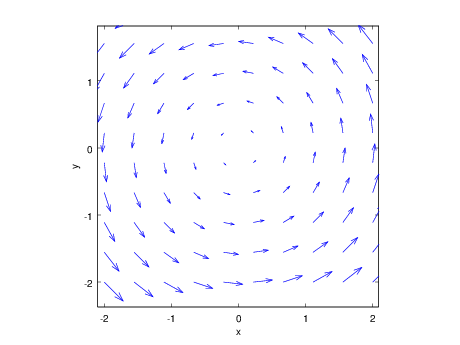
\includegraphics[width=0.700\linewidth]{vfield.png}\hfill}

\emph{Vigursviðið} \(\mathbf{F}(x,y) = -y\mbox{${\bf i}$}+ x \mbox{${\bf j}$}\).

\index{straumlína}

\section{Straumlína}
\label{Kafli5:straumlina}\label{Kafli5:index-1}

\subsection{Skilgreining}
\label{Kafli5:id2}
\textit{Ferill} \(C\) í planinu kallast \textit{straumlína} fyrir \textit{vigursvið} \(\mbox{${\bf F}$}(x,y)\) ef í hverjum punkti
\((x,y)\) á ferlinum er vigurinn \(\mbox{${\bf F}$}(x,y)\)
\textit{snertivigur} við ferilinn.

{\hfill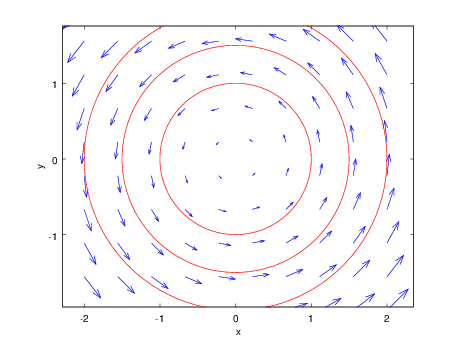
\includegraphics[width=0.700\linewidth]{flowlines.png}\hfill}

\emph{Vigursviðið} \(\mathbf{F}(x,y) = -y\mbox{${\bf i}$}+ x \mbox{${\bf j}$}\)
\emph{ásamt nokkrum straumlínum}.

\index{vigursvið:geymið}\index{stigulsvið}\index{mætti}

\section{Stigulsvið}
\label{Kafli5:index-2}\label{Kafli5:stigulsvi}

\subsection{Skilgreining}
\label{Kafli5:id3}
Vigursvið \(\mbox{${\bf F}$}(x,y)\) kallast \emph{stigulsvið} eða \emph{geymið
svið} (e. gradient field, conservative field) á mengi \(D\) ef til
er fall \(\varphi(x,y)\) þannig að
\begin{gather}
\begin{split}\displaystyle \mbox{${\bf F}$}(x,y)=\nabla\varphi(x,y)\end{split}\notag
\end{gather}
fyrir alla punkta \((x,y)\in D\), það er að segja ef
\begin{gather}
\begin{split}\displaystyle \mbox{${\bf F}$}(x,y)=F_1(x,y)\,\mbox{${\bf i}$}+F_2(x,y)\,\mbox{${\bf j}$}\end{split}\notag
\end{gather}
þá er
\begin{gather}
\begin{split}\displaystyle F_1(x,y)=\frac{\partial}{\partial x}\varphi(x,y) \quad \text{og}\quad  F_2(x,y)=\frac{\partial}{\partial y}\varphi(x,y).\end{split}\notag
\end{gather}
Vigursvið \(\mbox{${\bf F}$}(x,y,z)\) kallast \emph{stigulsvið} eða
\emph{geymið svið} ef til er fall \(\varphi(x,y,z)\) þannig að
\(\mbox{${\bf F}$}(x,y,z)=\nabla\varphi(x,y,z)\).

Fallið \(\varphi\) kallast \textit{mætti}  fyrir vigursviðið
\(\mbox{${\bf F}$}\).


\subsection{Setning}
\label{Kafli5:setning}
Látum
\(\mbox{${\bf F}$}(x,y)=F_1(x,y)\,\mbox{${\bf i}$}+F_2(x,y)\,\mbox{${\bf j}$}\)
vera vigursvið þannig að föllin \(F_1(x,y)\) og \(F_2(x,y)\)
hafi samfelldar hlutafleiður. Ef \(\mbox{${\bf F}$}(x,y)\) er
stigulsvið þá er
\begin{gather}
\begin{split}\displaystyle\end{split}\notag\\\begin{split}\frac{\partial}{\partial y}F_1(x,y)=
\frac{\partial}{\partial x}F_2(x,y).\end{split}\notag
\end{gather}
\begin{notice}{note}{Athugasemd:}
Þó að hlutafleiðurnar séu jafnar þá er \textbf{ekki} hægt að álykta að \(\mbox{${\bf F}$}\) sé stigulsvið. Þetta atriði verður rætt síðar.
\end{notice}


\subsection{Setning}
\label{Kafli5:id4}
Látum
\(\mbox{${\bf F}$}(x,y,z)=F_1(x,y,z)\,\mbox{${\bf i}$}+F_2(x,y,z)\,\mbox{${\bf j}$}+F_3(x,y,z)\,\mbox{${\bf k}$}\)
vera vigursvið þannig að föllin \(F_1(x,y,z), F_2(x,y,z)\) og
\(F_3(x,y,3)\) hafi samfelldar hlutafleiður. Ef
\(\mbox{${\bf F}$}(x,y,z)\) er stigulsvið þá er
\begin{gather}
\begin{split}\displaystyle\end{split}\notag\\\begin{split}\begin{aligned}
\frac{\partial}{\partial y}F_1(x,y,z) &=
\frac{\partial}{\partial x}F_2(x,y,z), \\
\frac{\partial}{\partial z}F_1(x,y,z) &=
\frac{\partial}{\partial x}F_3(x,y,z) \quad \text{og} \\
\frac{\partial}{\partial z}F_2(x,y,z)&=
\frac{\partial}{\partial y}F_3(x,y,z).\end{aligned}\end{split}\notag
\end{gather}

\subsection{Reikniaðferð}
\label{Kafli5:reikniafer}
Finna á \textit{mætti} \(\varphi(x,y)\) fyrir stigulsvið
\(\mbox{${\bf F}$}(x,y)=F_1(x,y)\,\mbox{${\bf i}$}+F_2(x,y)\,\mbox{${\bf j}$}\).
Viljum finna fall \(\varphi(x,y)\) þannig að
\begin{gather}
\begin{split}\displaystyle\end{split}\notag\\\begin{split}\frac{\partial}{\partial x}\varphi(x,y)=F_1(x,y)\qquad
\mbox{og}\qquad \frac{\partial}{\partial y}\varphi(x,y)=F_2(x,y).\end{split}\notag
\end{gather}
Með því að heilda þessar jöfnur fæst að
\begin{gather}
\begin{split}\displaystyle \varphi(x,y)=\int F_1(x,y)\,dx+C_1(y)\end{split}\notag\\\begin{split}og\end{split}\notag
\end{gather}\begin{gather}
\begin{split}\displaystyle \varphi(x,y)=\int F_2(x,y)\,dy+C_2(x).\end{split}\notag
\end{gather}
Þegar fyrra stofnfallið er reiknað þá er \(y\) hugsað sem fasti og
því fæst heildunarfasti sem getur verið fall af \(y\). Lokaskrefið
er svo að horfa á jöfnurnar tvær hér að ofan og sjá hvort ekki er hægt
að finna gildi fyrir heildunarfastanna \(C_1(x)\) og \(C_2(y)\)
þannig að sama formúlan fyrir \(\varphi(x,y)\) fáist.

\index{ferilheildi}

\section{Heildi falls yfir feril}
\label{Kafli5:index-3}\label{Kafli5:heildi-falls-yfir-feril}

\subsection{Skilgreining}
\label{Kafli5:id5}
Látum \(\cal C\) vera feril í \({\mathbb  R}^2\) stikaðan af
samfellt diffranlegum stikaferli
\(\mbox{${\bf r}$}:[a,b]\rightarrow{\mathbb  R}^2\). Ritum
\(\mbox{${\bf r}$}(t)=(x(t),y(t))\). \emph{Heildi falls} \(f(x,y)\)
\emph{yfir ferilinn} \(\cal C\) \emph{með tilliti til bogalengdar} er
skilgreint sem
\begin{gather}
\begin{split}\displaystyle\end{split}\notag\\\begin{split}\begin{aligned}
\int_{\cal C}f(x,y)\,ds&=\int_a^b f(\mbox{${\bf r}$}(t))\,|\mbox{${\bf r}$}'(t)|\,dt\\
&=\int_a^b f(x(t),y(t))\,\sqrt{x'(t)^2+y'(t)^2}\,dt.\end{aligned}\end{split}\notag
\end{gather}
Sama aðferð notuð til að skilgreina heildi falls yfir feril í
\({\mathbb  R}^3\).


\subsection{Setning}
\label{Kafli5:id6}
Látum \(\cal C\) vera feril í \({\mathbb  R}^2\). Gerum ráð
fyrir að \(\mbox{${\bf r}$}_1\) og \(\mbox{${\bf r}$}_2\) séu
tveir samfellt diffranlegir stikaferlar sem báðir stika ferilinn
\(\cal C\). Ef fall \(f(x,y)\) er heildað yfir \(\cal C\) þá
fæst sama útkoma hvort sem stikunin \(\mbox{${\bf r}$}_1\) eða
stikunin \(\mbox{${\bf r}$}_2\) er notuð við útreikningana.


\subsection{Skilgreining}
\label{Kafli5:id7}
Ferill \(\cal C\) í plani er sagður \emph{samfellt diffranlegur á köflum}
ef til er stikun
\(\mbox{${\bf r}$}:[a,b]\rightarrow {\mathbb  R}^2\) á
\(\cal C\) þannig að til eru punktar
\(a=t_0<t_1<t_2<\cdots<t_n<t_{n+1}=b\) þannig að á hverju bili
\((t_i,t_{i+1})\) er \(\mbox{${\bf r}$}\) \textit{samfellt diffranlegur}
ferill og \textit{markgildin}
\begin{gather}
\begin{split}\displaystyle\end{split}\notag\\\begin{split}\lim_{t\rightarrow t_i^+}\mbox{${\bf r}$}'(t)\qquad\mbox{og}\qquad
\lim_{t\rightarrow t_{i+1}^-}\mbox{${\bf r}$}'(t)\end{split}\notag
\end{gather}
eru bæði til.

Líka sagt að stikaferillinn \(\mbox{${\bf r}$}\) sé \emph{samfellt
diffranlegur á köflum.}


\section{Heildi vigursviðs eftir ferli}
\label{Kafli5:heildi-vigursvis-eftir-ferli}

\subsection{Skilgreining}
\label{Kafli5:id8}
Látum \(\mbox{${\bf F}$}(x,y)\) vera vigursvið og
\(\mbox{${\bf r}$}:[a,b]\rightarrow {\mathbb  R}^2\) stikun á ferli
\(\cal C\) og gerum ráð fyrir að stikaferillinn
\(\mbox{${\bf r}$}\) sé samfellt diffranlegur á köflum. \emph{Heildi
vigursviðsins} \(\mbox{${\bf F}$}(x,y)\) \emph{eftir ferlinum}
\(\cal C\) er skilgreint sem
\begin{gather}
\begin{split}\displaystyle\end{split}\notag\\\begin{split}\int_{\cal C} \mbox{${\bf F}$}\cdot d\mbox{${\bf r}$}= \int_{\cal C} \mbox{${\bf F}$}\cdot \mbox{${\bf T}$}\,ds
=\int_a^b \mbox{${\bf F}$}(\mbox{${\bf r}$}(t))\cdot \mbox{${\bf r}$}'(t)\,dt.\end{split}\notag
\end{gather}

\subsection{Skilgreining}
\label{Kafli5:id9}
Ritum
\(\mbox{${\bf F}$}(x,y)=F_1(x,y)\,\mbox{${\bf i}$}+F_2(x,y)\,\mbox{${\bf j}$}\).
Ritum líka
\(\mbox{${\bf r}$}(t)=x(t)\,\mbox{${\bf i}$}+y(t)\,\mbox{${\bf j}$}\).
Þá má rita \(dx=x'(t)\,dt,\, dy=y'(t)\,dt\). Með því að nota þennan
rithátt fæst að
\begin{gather}
\begin{split}\displaystyle\end{split}\notag\\\begin{split}\begin{aligned}
\int_{\cal C}\mbox{${\bf F}$}\cdot d\mbox{${\bf r}$}&=\int_a^b
(F_1(x,y)\,\mbox{${\bf i}$}+F_2(x(t),y(t))\,\mbox{${\bf j}$})\cdot(x'(t)\,\mbox{${\bf i}$}+y'(t)\,\mbox{${\bf j}$})\,dt\\
&=\int_a^b F_1(x(t),y(t))x'(t)\,dt+F_2(x(t),y(t))y'(t)\,dt\\
&=\int_{\cal C} F_1(x,y)\,dx+F_2(x,y)\,dy.\end{aligned}\end{split}\notag
\end{gather}
\begin{notice}{note}{Athugasemd:}
Látum \(\cal C\) vera feril í \({\mathbb  R}^2\). Gerum ráð fyrir að \(\mbox{${\bf r}$}_1:[a,b]\rightarrow {\mathbb  R}^2\) og \(\mbox{${\bf r}$}_2:[a',b']\rightarrow {\mathbb  R}^2\) séu tveir samfellt diffranlegir á köflum stikaferlar sem stika \(\cal C\). Gerum ennfremur ráð fyrir að \(\mbox{${\bf r}$}_1(a)=\mbox{${\bf r}$}_2(b')\) og \(\mbox{${\bf r}$}_1(b)=\mbox{${\bf r}$}_2(a')\) (þ.e.a.s. stikaferlarnir fara í sitthvora áttina eftir \(\cal C\)). Þá gildir ef \(\mbox{${\bf F}$}(x,y)\) er vigursvið að
\begin{gather}
\begin{split}\displaystyle \int_{\cal C} \mbox{${\bf F}$}\cdot d\mbox{${\bf r}$}_1=-\int_{\cal C} \mbox{${\bf F}$}\cdot d\mbox{${\bf r}$}_2.\end{split}\notag
\end{gather}
(Ef breytt er um stefnu á stikun á breytist formerki þegar vigursvið heildað eftir ferlinum.)
\end{notice}


\section{Ferilheildi og stigulsvið}
\label{Kafli5:ferilheildi-og-stigulsvi}

\subsection{Setning}
\label{Kafli5:id10}
Látum \(\mbox{${\bf F}$}(x,y)\) vera samfellt stigulsvið skilgreint
á svæði \(D\) í \({\mathbb  R}^2\) og látum \(\varphi\) vera
fall skilgreint á \(D\) þannig að
\(\mbox{${\bf F}$}(x,y)=\nabla \varphi(x,y)\) fyrir alla punkta
\((x,y)\in D\). Látum \(\mbox{${\bf r}$}:[a,b]\rightarrow D\)
vera stikaferill sem er samfellt diffranlegur á köflum og stikar feril
\(\cal C\) í \(D\). Þá er
\begin{gather}
\begin{split}\displaystyle \int_{\cal C} \mbox{${\bf F}$}\cdot \,d\mbox{${\bf r}$}=\varphi(\mbox{${\bf r}$}(b))-\varphi(\mbox{${\bf r}$}(a)).\end{split}\notag
\end{gather}
(Samsvarandi gildir fyrir vigursvið skilgreint á svæði
\(D\subseteq {\mathbb  R}^3\).)


\subsection{Fylgisetning}
\label{Kafli5:fylgisetning}
Látum \(\mbox{${\bf F}$}\) vera samfellt stigulsvið skilgreint á
mengi \(D\subseteq {\mathbb  R}^2\). Látum
\(\mbox{${\bf r}$}:[a,b]\rightarrow D\) vera stikaferil sem er
samfellt diffranlegur á köflum og lokaður (þ.e.a.s.
\(\mbox{${\bf r}$}(a)=\mbox{${\bf r}$}(b)\)) og stikar feril
\(\mathcal{C}\). Þá er
\begin{gather}
\begin{split}\displaystyle \oint_{\cal C}  \mbox{${\bf F}$}\cdot \,d\mbox{${\bf r}$}=0.\end{split}\notag
\end{gather}
(Ath. að rithátturinn
\begin{gather}
\begin{split}\displaystyle \oint_{\cal C}\end{split}\notag
\end{gather}
er gjarnan notaður þegar heildað er yfir lokaðan feril \(\cal C\).)


\subsection{Fylgisetning}
\label{Kafli5:id11}
Látum \(\mbox{${\bf F}$}\) vera samfellt stigulsvið skilgreint á
mengi \(D\subseteq {\mathbb  R}^2\). Látum
\(\mbox{${\bf r}$}_1:[a_1,b_1]\rightarrow D\) og
\(\mbox{${\bf r}$}_2:[a_2,b_2]\rightarrow D\) vera stikaferla sem
eru samfellt diffranlegir á köflum og stika ferlana
\(\mathcal{C}_1\) og \(\mathcal{C}_2\). Gerum ráð fyrir að
\(\mbox{${\bf r}$}_1(a_1)=\mbox{${\bf r}$}_2(a_2)\) og
\(\mbox{${\bf r}$}_1(b_1)=\mbox{${\bf r}$}_2(b_2)\),
þ.e.a.s. stikaferlarnir \(\mbox{${\bf r}$}_1\) og
\(\mbox{${\bf r}$}_2\) hafa sameiginlega upphafs- og endapunkta. Þá
er
\begin{gather}
\begin{split}\displaystyle \int_{{\cal C}_1} \mbox{${\bf F}$}\cdot\,d\mbox{${\bf r}$}_1=\int_{{\cal C}_2} \mbox{${\bf F}$}\cdot\,d\mbox{${\bf r}$}_2.\end{split}\notag
\end{gather}

\subsection{Skilgreining}
\label{Kafli5:id12}
Segjum að heildi vigursviðs \(\mbox{${\bf F}$}\) sé \emph{óháð
stikaferli} ef fyrir sérhverja tvo samfellt diffranlega á köflum
stikaferla \(\mbox{${\bf r}$}_1\) og \(\mbox{${\bf r}$}_2\) með
sameiginlega upphafs- og endapunkta sem stika ferlana
\(\mathcal{C}_1\) og \(\mathcal{C}_2\) gildir að
\begin{gather}
\begin{split}\displaystyle\end{split}\notag\\\begin{split}\int_{{\cal C}_1} \mbox{${\bf F}$}\cdot\,d\mbox{${\bf r}$}_1=
\int_{{\cal C}_2} \mbox{${\bf F}$}\cdot\,d\mbox{${\bf r}$}_2.\end{split}\notag
\end{gather}

\subsection{Setning}
\label{Kafli5:id13}
Ferilheildi samfellds vigursviðs \(\mbox{${\bf F}$}\) er óháð
stikaferli ef og aðeins ef
\(\oint_{\cal C} \mbox{${\bf F}$}\cdot\,d\mbox{${\bf r}$}=0\) fyrir
alla lokaða ferla \(\cal C\) sem eru samfellt diffranlegir á köflum.


\subsection{Upprifjun}
\label{Kafli5:upprifjun}
Segjum að mengi \(D\subseteq {\mathbb  R}^2\) sé
\emph{ferilsamanhangandi} (e. connected, path-connected) ef fyrir sérhverja
tvo punkta \(P, Q\in D\) gildir að til er stikaferill
\(\mbox{${\bf r}$}:[0,1]\rightarrow D\) þannig að
\(\mbox{${\bf r}$}(0)=P\) og \(\mbox{${\bf r}$}(1)=Q\).


\subsection{Setning}
\label{Kafli5:id14}
Látum \(D\) vera \textit{opið mengi} í \({\mathbb  R}^2\) sem er
ferilsamanhangandi. Ef \(\mbox{${\bf F}$}\) er samfellt vigursvið
skilgreint á \(D\) og ferilheildi \(\mbox{${\bf F}$}\) eru óháð
vegi þá er \(\mbox{${\bf F}$}\) stigulsvið.


\subsection{Setning}
\label{Kafli5:id15}
Fyrir samfellt vigursvið \(\mbox{${\bf F}$}\) skilgreint á opnu
ferilsamanhangandi mengi \(D\subseteq {\mathbb  R}^2\) er
eftirfarandi jafngilt:
\begin{enumerate}
\item {} 
\(\mbox{${\bf F}$}\) er stigulsvið,

\item {} 
\(\oint_{\cal C} \mbox{${\bf F}$}\cdot\,d\mbox{${\bf r}$}=0\) fyrir alla samfellt diffranlega á köflum lokaða stikaferla \(\mbox{${\bf r}$}\) í \(D\),

\item {} 
Ferilheildi \(\mbox{${\bf F}$}\) er óháð vegi.

\end{enumerate}
\begin{enumerate}
\item {} 
\(\Rightarrow\) (b). Fylgisetning 5.6.2.

\item {} 
\(\Leftrightarrow\) (c). Setning 5.6.5.

\item {} 
\(\Rightarrow\) (a). Setning 5.6.7.

\end{enumerate}

\index{flötur}

\section{Fletir}
\label{Kafli5:index-4}\label{Kafli5:fletir}

\subsection{Óformleg skilgreining}
\label{Kafli5:oformleg-skilgreining}
\textit{Flötur} \(\cal S\) í \({\mathbb  R}^3\) er ,,tvívítt hlutmengi í
\({\mathbb  R}^3\).


\subsection{Lýsing}
\label{Kafli5:lysing}
Flötum er aðallega lýst með formúlum á þrjá vegu:
\begin{enumerate}
\item {} 
Gefið er fall \(f(x,y,z)\). Fletinum \(\cal S\) er lýst með
jöfnu \(f(x,y,z)=C\) (þ.e.a.s. \(\cal S\) er \textit{jafnhæðarflötur}
fallsins \(f\)). Þá er
\begin{gather}
\begin{split}\displaystyle {\cal S}=\{(x,y,z)\mid f(x,y,z)=C\}.\end{split}\notag
\end{gather}
\item {} 
Gefið er fall skilgreint á ferilsamanhangandi svæði \(D\) í
\({\mathbb  R}^2\). Fletinum \(\cal S\) er lýst sem grafi
fallsins \(f\). Þá er
\begin{gather}
\begin{split}\displaystyle {\cal S}=\{(x,y,z)\mid (x,y)\in D\mbox{ og } z=f(x,y)\}.\end{split}\notag
\end{gather}
\item {} 
Með stikafleti (sjá næstu grein).

\end{enumerate}

\index{stikaflötur}

\section{Stikafletir}
\label{Kafli5:index-5}\label{Kafli5:stikafletir}

\subsection{Skilgreining}
\label{Kafli5:id16}
Látum \(D\) vera ferilsamanhangandi hlutmengi í
\({\mathbb  R}^2\). Samfelld vörpun
\(\mbox{${\bf r}$}:D\rightarrow {\mathbb  R}^3; \mbox{${\bf r}$}(u,v)=\big(x(u,v), y(u,v), z(u,v)\big)\)
þannig að
\begin{gather}
\begin{split}\displaystyle {\cal S}=\{\mbox{${\bf r}$}(u,v)\mid (u,v)\in D\}\end{split}\notag
\end{gather}
er flötur kallast \emph{stikaflötur}. Segjum að \(\mbox{${\bf r}$}\) sé
\emph{stikun á fletinum} \(\cal S\). Viljum að \(\mbox{${\bf r}$}\)
sé eintæk vörpun, nema hugsanlega á jaðri \(D\). Ritum einnig
\begin{gather}
\begin{split}\displaystyle\end{split}\notag\\\begin{split}\frac{\partial \mbox{${\bf r}$}}{\partial u}=
\bigg(\frac{\partial x}{\partial u}, \frac{\partial y}{\partial u},
\frac{\partial z}{\partial u}\bigg)\quad\mbox{ og }\quad
\frac{\partial \mbox{${\bf r}$}}{\partial v}=
\bigg(\frac{\partial x}{\partial v}, \frac{\partial y}{\partial v},
\frac{\partial z}{\partial v}\bigg).\end{split}\notag
\end{gather}

\section{Snertiplön}
\label{Kafli5:snertiplon}

\subsection{Setning}
\label{Kafli5:id17}\begin{enumerate}
\item {} 
Látum \(\cal S\) vera flöt sem er gefinn sem \textit{jafnhæðarflötur}
\(f(x,y,z)=C\). Ef \((a, b, c)\) er punktur á fletinum og
fallið \(f\) er diffranlegt í punktinum \((a, b,c)\) þá er
vigurinn \(\mbox{${\bf n}$}=\nabla f(a, b, c)\) hornréttur á
flötinn í punktinum \((a,b, c)\) og ef
\(\nabla f(a, b, c)\neq \mbox{${\bf 0}$}\) þá hefur flöturinn
\textit{snertiplan} í punktinum. Jafna snertiplansins er
\begin{gather}
\begin{split}\displaystyle f_1(a, b, c)x+f_2(a, b, c)y+f_3(a, b, c)z=D\end{split}\notag
\end{gather}
þar sem
\begin{gather}
\begin{split}\displaystyle\end{split}\notag\\\begin{split}D= f_1(a, b, c)a+f_2(a, b, c)b
+f_3(a, b, c)c.\end{split}\notag
\end{gather}
\item {} 
Látum \(\cal S\) vera flöt sem er gefinn sem graf falls
\(z=f(x,y)\). Ef \((a, b, f(a,b))\) er punktur á fletinum og
fallið \(f\) er diffranlegt í punktinum \((a, b)\) þá er
vigurinn
\begin{gather}
\begin{split}\displaystyle \mbox{${\bf n}$}=\big(0 ,1 ,f_2(a, b)\big)\times\big(1 ,0 ,f_1(a, b)\big)=\big(f_1(a, b), f_2(a, b), -1\big)\end{split}\notag
\end{gather}
hornréttur á flötinn í punktinum \((a,b, f(a,b))\) og flöturinn
hefur snertiplan í punktinum. Jafna snertiplansins er
\begin{gather}
\begin{split}\displaystyle z=f(a, b)+f_1(a, b)(x-a)+f_2(a, b)(y-b).\end{split}\notag
\end{gather}
\end{enumerate}

{\hfill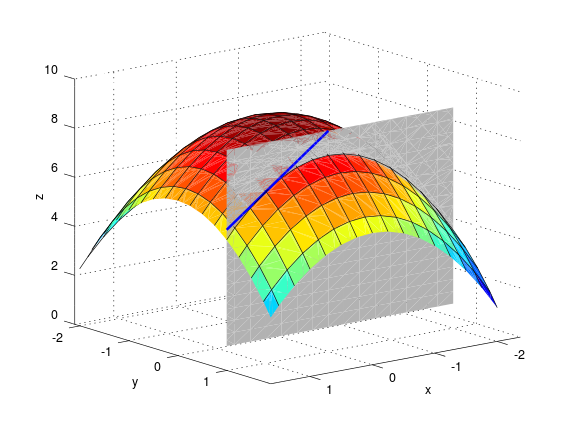
\includegraphics[width=0.700\linewidth]{xpart.png}\hfill}

\emph{Snertivigur við skurðferil sléttunnar} \(y=b\) \emph{og yfirborðsins} \(z = f(x,y)\) \emph{í punktinum} \((a,b,f(a,b))\) \emph{er} \(\mathbf{T}_1 = (1,0,f_1(a,b))\).

{\hfill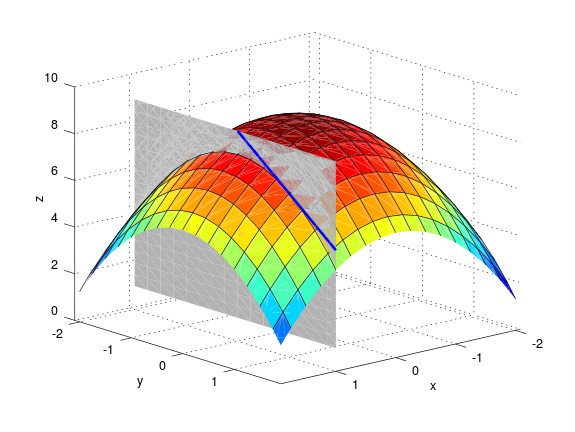
\includegraphics[width=0.700\linewidth]{ypart.png}\hfill}

\emph{Snertivigur við skurðferil sléttunnar} \(x=a\) \emph{og yfirborðsins} \(z = f(x,y)\) \emph{í punktinum} \((a,b,f(a,b))\) \emph{er} \(\mathbf{T}_2 = (0,1,f_2(a,b))\).
\begin{enumerate}
\setcounter{enumi}{2}
\item {} 
Látum
\(\mbox{${\bf r}$}: D\subseteq {\mathbb  R}^2\rightarrow {\mathbb  R}^3\)
vera stikaflöt. Ef \((x_0, y_0, z_0)=\mbox{${\bf r}$}(u_0, v_0)\)
er punktur á fletinum sem
\(\mbox{${\bf r}$}(u,v)=\big(x(u,v), y(u,v), z(u,v)\big)\) stikar
og föllin \(x(u,v), y(u,v), z(u,v)\) eru diffranleg í punktinum
\((x_0,
y_0)\) þá er vigurinn
\begin{gather}
\begin{split}\displaystyle\end{split}\notag\\\begin{split}\mbox{${\bf n}$}=\frac{\partial \mbox{${\bf r}$}}{\partial u}\times
\frac{\partial \mbox{${\bf r}$}}{\partial v}\end{split}\notag
\end{gather}
reiknaður með \(u=u_0\) og \(v=v_0\) þvervigur á flötinn í
punktinum \((x_0, y_0, z_0)\).

\end{enumerate}

\index{stikun!regluleg}

\subsection{Skilgreining}
\label{Kafli5:id18}\label{Kafli5:index-6}
Ef vigrarnir \(\frac{\partial \mbox{${\bf r}$}}{\partial u}(u,v)\)
og \(\frac{\partial \mbox{${\bf r}$}}{\partial v}(u,v)\) eru óháðir
fyrir alla punkta \((u,v)\in D\) þá er sagt að stikunin sé
\emph{regluleg}.

\begin{notice}{note}{Athugasemd:}
Ef vigrarnir \(\frac{\partial \mbox{${\bf r}$}}{\partial u}(u_0,v_0)\) og \(\frac{\partial\mbox{${\bf r}$}}{\partial v}(u_0,v_0)\) eru óháðir þá spanna þeir snertiplan við flötinn í punktinum \(\mbox{${\bf r}$}(u_0,v_0)\). Snertiplanið hefur stikun
\begin{gather}
\begin{split}\displaystyle
\Pi(u,v) = \mbox{${\bf r}$}(u_0,v_0)+u\frac{\partial \mbox{${\bf r}$}}{\partial u}(u_0,v_0)+v\frac{\partial \mbox{${\bf r}$}}{\partial v}(u_0,v_0).\end{split}\notag
\end{gather}\end{notice}

\index{flatarheildi}

\section{Flatarheildi}
\label{Kafli5:index-7}\label{Kafli5:flatarheildi}

\subsection{Verkefni}
\label{Kafli5:verkefni}\begin{enumerate}
\item {} 
Flatarmál flata – sambærilegt við bogalengd ferla.

\item {} 
Heildi falls yfir flöt með tilliti til flatarmáls – sambærilegt við
heildi falls eftir ferli með tilliti til bogalengdar.

\item {} 
Heildi vigursviðs yfir flöt – svipar til heildis vigursviðs eftir
ferli.

\end{enumerate}


\section{Flatarmál flata}
\label{Kafli5:flatarmal-flata}

\subsection{Skilgreining}
\label{Kafli5:id19}
Látum \(\mbox{${\bf r}$}:D\rightarrow {\mathbb  R}^2\) vera
reglulegan stikaflöt sem stikar flöt \(\cal S\). Flatarmál
\(\cal S\) er
\begin{gather}
\begin{split}\displaystyle\end{split}\notag\\\begin{split}A=\int\!\!\!\int_D\,dS=\int\!\!\!\int_D \big|{\textstyle\frac{\partial \mbox{${\bf r}$}}{\partial u}
\times\frac{\partial \mbox{${\bf r}$}}{\partial v}}\big|\,dudv.\end{split}\notag
\end{gather}

\subsection{Formúla}
\label{Kafli5:formula}
Látum \(f(x,y)\) vera diffranlegt fall skilgreint á mengi \(D\)
í \({\mathbb  R}^2\). Flatarmál grafsins \(z=f(x,y)\) er gefið
með formúlunni
\begin{gather}
\begin{split}\displaystyle\end{split}\notag\\\begin{split}A=\int\!\!\!\int_D dS=\int\!\!\!\int_D {\textstyle\sqrt{1+
\big(\frac{\partial f}{\partial x}\big)^2+
\big(\frac{\partial f}{\partial y}\big)^2}}\,\,dx\,dy.\end{split}\notag
\end{gather}

\subsection{Skilgreining}
\label{Kafli5:id20}
Látum \(\mbox{${\bf r}$}:D\rightarrow {\mathbb  R}^3\) vera
reglulegan stikaflöt sem stikar flöt \(\cal S\). Flatarmál
\(\cal S\) er
\begin{gather}
\begin{split}\displaystyle\end{split}\notag\\\begin{split}A=\int\!\!\!\int_D\,dS=\int\!\!\!\int_D \big|{\textstyle\frac{\partial \mbox{${\bf r}$}}{\partial u}
\times\frac{\partial \mbox{${\bf r}$}}{\partial v}}\big|\,dudv.\end{split}\notag
\end{gather}

\subsection{Formúla}
\label{Kafli5:id21}
Látum \(f(x,y)\) vera diffranlegt fall skilgreint á mengi \(D\)
í \({\mathbb  R}^2\). Flatarmál grafsins \(z=f(x,y)\) er gefið
með formúlunni
\begin{gather}
\begin{split}\displaystyle\end{split}\notag\\\begin{split}A=\int\!\!\!\int_D dS=\int\!\!\!\int_D {\textstyle\sqrt{1+
\big(\frac{\partial f}{\partial x}\big)^2+
\big(\frac{\partial f}{\partial y}\big)^2}}\,\,dx\,dy.\end{split}\notag
\end{gather}

\subsection{Formúlur}
\label{Kafli5:formulur}
Ritum \(dS\) fyrir flatarmálselement á fleti \(\cal S\).
\begin{itemize}
\item {} 
Ef
\(\mbox{${\bf r}$}:D\subseteq{\mathbb  R}^2\rightarrow {\mathbb  R}^3\)
er stikun á \(\cal S\) þá er
\begin{gather}
\begin{split}\displaystyle\end{split}\notag\\\begin{split}dS=\bigg|\frac{\partial \mbox{${\bf r}$}}{\partial u}\times\frac{\partial
  \mbox{${\bf r}$}}{\partial v}\bigg|\,du\,dv.\end{split}\notag
\end{gather}
\item {} 
Ef \(\cal S\) er graf \(z=g(x,y)\) þá er
\begin{gather}
\begin{split}\displaystyle dS=\sqrt{1+g_1(x,y)^2+g_2(x,y)^2}\,dx\,dy.\end{split}\notag
\end{gather}
\item {} 
Gerum ráð fyrir að flöturinn \(\cal S\) í \({\mathbb  R}^3\)
hafi þann eiginleika að ofanvarp hans á \(xy\)-planið sé eintækt
eða með öðrum orðum hægt er að lýsa fletinum sem grafi
\(z=f(x,y)\). Ef \(\mbox{${\bf n}$}\) er þvervigur á flötinn
og \(\gamma\) er hornið sem \textit{þvervigurinn} \(\mbox{${\bf n}$}\)
myndar við jákvæða hluta \(z\)-ássins þá er
\begin{gather}
\begin{split}\displaystyle\end{split}\notag\\\begin{split}dS=\bigg|\frac{1}{\cos\gamma}\bigg|\,dx\,dy
=\frac{|\mbox{${\bf n}$}|}{|\mbox{${\bf n}$}\cdot\mbox{${\bf k}$}|}\,dx\,dy.\end{split}\notag
\end{gather}
Í þessu tilviki gildir einnig að ef \(\cal S\) er lýst sem
hæðarfleti \(G(x,y,z)=C\) þá er
\begin{gather}
\begin{split}\displaystyle dS=\bigg|\frac{\nabla G(x,y,z)}{G_3(x,y,z)}\bigg|\,dx\,dy.\end{split}\notag
\end{gather}
\end{itemize}


\subsection{Skilgreining}
\label{Kafli5:id22}
Látum \(\mbox{${\bf r}$}: D\rightarrow {\mathbb  R}^3\) vera
reglulega stikun á fleti \(\cal S\). Heildi falls \(f(x,y,z)\)
yfir flötinn \(\cal S\) með tilliti til flatarmáls er
\begin{gather}
\begin{split}\displaystyle\end{split}\notag\\\begin{split}\int\!\!\!\int_{\cal S} f\,dS=\int\!\!\!\int_D f(\mbox{${\bf r}$}(u,v)) \big|{\textstyle\frac{\partial
    \mbox{${\bf r}$}}{\partial u}
\times\frac{\partial \mbox{${\bf r}$}}{\partial v}}\big|\,dudv.\end{split}\notag
\end{gather}
\index{einingarþvervigrasvið}

\section{Einingarþvervigrasvið}
\label{Kafli5:index-8}\label{Kafli5:einingarvervigrasvi}

\subsection{Skilgreining}
\label{Kafli5:id23}
Látum \(\cal S\) vera flöt í \({\mathbb  R}^3\) sem hefur \textit{snertiplan} í punkti \(P\).
\emph{Einingarþvervigur} \(\mbox{${\bf n}$}\) á flötinn \(\cal S\) í
punktinum \(P\) er \textit{einingarvigur} hornréttur á snertiplan við flötinn
í punktinum \(P\).

\emph{Einingarþvervigrasvið} á \(\cal S\) er samfellt \textit{vigursvið}
\(\mbox{${\bf N}$}\) sem er skilgreint í öllum punktum
\(\cal S\) þannig að fyrir \((x,y,z)\in{\cal S}\) er vigurinn
\(\mbox{${\bf n}$}(x,y,z)\) einingarvigur sem er hornréttur á
snertiplan við flötinn í punktinum \((x,y,z)\).

{\hfill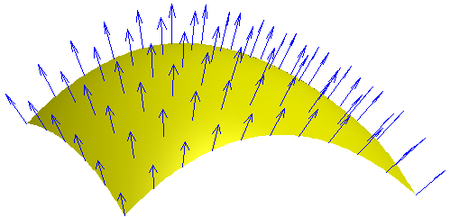
\includegraphics[width=0.500\linewidth]{normalfield.png}\hfill}

\index{flötur!áttanlegur}\index{áttun}

\section{Áttanlegir fletir}
\label{Kafli5:index-9}\label{Kafli5:attanlegir-fletir}

\subsection{Skilgreining}
\label{Kafli5:id24}
Flöturinn \(\cal S\) er sagður \textit{áttanlegur} ef til er
einingarþvervigrasvið \(\mbox{${\bf N}$}\) á \(\cal S\).

\textit{Áttun} á áttanlegum fleti felst í því að velja annað af tveimur mögulegum
einingaþvervigrasviðum.

{\hfill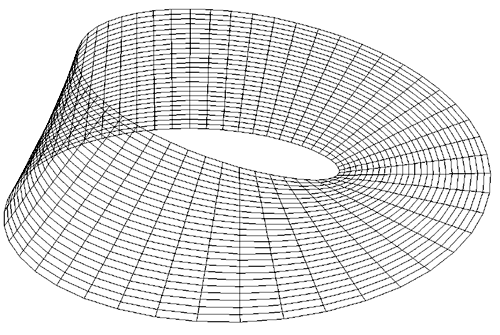
\includegraphics[width=0.400\linewidth]{mobius.png}\hfill}

\emph{Möbiusarborði er ekki áttanlegur.}


\subsection{Umræða}
\label{Kafli5:umraea}
Ef áttanlegur flötur \(\cal S\) hefur jaðar þá skilgreinir áttunin
stefnu á jaðri \(\cal S\). Venjan er að velja stefnu jaðarsins
þannig að þegar gengið er eftir honum sé einingarþvervigrasviðið á
vinstri hönd (hægri handar regla).

Ef tveir áttanlegir fletir hafa jaðar má splæsa þeim saman í áttanlegan
flöt með því að líma þá saman á (hluta af) jöðrunum og gæta þess að
jaðrarnir hafi andstæða stefnu á samskeytunum.

{\hfill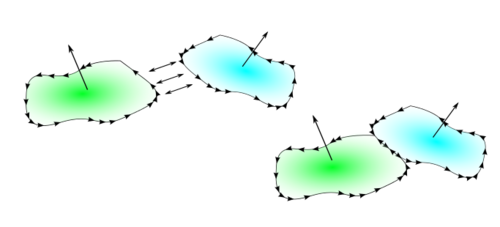
\includegraphics[width=0.700\linewidth]{joinsurf.png}\hfill}


\subsection{Setning}
\label{Kafli5:id25}
Gerum ráð fyrir að \(\cal S\) sé \textit{áttanlegur} flötur og
\(\mbox{${\bf r}$}:D\subseteq{\mathbb  R}^2\rightarrow {\mathbb  R}^3\)
sé regluleg stikun á \(\cal S\) (það er,
\(\frac{\partial \mbox{${\bf r}$}}{\partial u}\) og
\(\frac{\partial \mbox{${\bf r}$}}{\partial v}\) eru samfelld föll
af \(u\) og \(v\) og vigrarnir
\(\frac{\partial \mbox{${\bf r}$}}{\partial u}\) og
\(\frac{\partial \mbox{${\bf r}$}}{\partial v}\) eru línulega
óháðir). Þá er
\begin{gather}
\begin{split}\displaystyle\end{split}\notag\\\begin{split}\mbox{${\bf N}$}=
\frac{\frac{\partial \mbox{${\bf r}$}}{\partial u}\times\frac{\partial
    \mbox{${\bf r}$}}{\partial v}}
{|\frac{\partial \mbox{${\bf r}$}}{\partial u}\times\frac{\partial
    \mbox{${\bf r}$}}{\partial v}|}\end{split}\notag
\end{gather}
einingarþvervigrasvið á \(\cal S\).

\index{flæði}

\section{Heildi vigursviðs yfir flöt - Flæði}
\label{Kafli5:heildi-vigursvis-yfir-flot-flaei}\label{Kafli5:index-10}

\subsection{Skilgreining og ritháttur}
\label{Kafli5:skilgreining-og-rithattur}
Látum \(\cal S\) vera \textit{áttanlegan} flöt stikaðan af reglulegum
stikaferli
\(\mbox{${\bf r}$}:D\subseteq{\mathbb  R}^2\rightarrow {\mathbb  R}^3\)
með samfelldar hlutafleiður. Látum \(\mbox{${\bf N}$}\) tákna
einingarþvervigrasviðið sem gefið er í Setningu 5.13.3. Heildi vigursviðs
\(\mbox{${\bf F}$}\) yfir flötinn \(\cal S\) er skilgreint sem
\begin{gather}
\begin{split}\displaystyle\end{split}\notag\\\begin{split}\int\!\!\!\int_{\cal S} \mbox{${\bf F}$}\cdot\mbox{${\bf N}$}\,dS
=\int\!\!\!\int_D \mbox{${\bf F}$}(\mbox{${\bf r}$}(u,v))\cdot \bigg(
\frac{\partial \mbox{${\bf r}$}}{\partial u}\times\frac{\partial \mbox{${\bf r}$}}{\partial
  v}\bigg)\,
du\,dv.\end{split}\notag
\end{gather}
Slík heildi eru oft nefnd \textit{flæði} vigursviðsins \(\mbox{${\bf F}$}\)
gegnum flötinn \(\cal S\).

Ritum \(d\mbox{${\bf S}$}=\mbox{${\bf N}$}\,dS\). Þá er
\begin{gather}
\begin{split}\displaystyle \int\!\!\!\int_{\cal S} \mbox{${\bf F}$}\cdot\mbox{${\bf N}$}\,dS=\int\!\!\!\int_{\cal S} \mbox{${\bf F}$}\cdot\,d\mbox{${\bf S}$}.\end{split}\notag
\end{gather}

\subsection{Samantekt}
\label{Kafli5:samantekt}\begin{enumerate}
\item {} 
Ef
\(\mbox{${\bf r}$}:D\subseteq{\mathbb  R}^2\rightarrow {\mathbb  R}^3\)
er stikun á \(\cal S\) þá er
\begin{gather}
\begin{split}\displaystyle\end{split}\notag\\\begin{split}d\mbox{${\bf S}$}=\pm \bigg(\frac{\partial \mbox{${\bf r}$}}{\partial u}\times\frac{\partial
  \mbox{${\bf r}$}}{\partial v}\bigg)\,du\,dv.\end{split}\notag
\end{gather}
\item {} 
Ef \(\cal S\) er graf \(z=f(x,y)\) þá er
\begin{gather}
\begin{split}\displaystyle\end{split}\notag\\\begin{split}d\mbox{${\bf S}$}=\pm\bigg(-\frac{\partial f}{\partial x},-\frac{\partial
  f}{\partial y},1\bigg)\,dx\,dy.\end{split}\notag
\end{gather}
\item {} 
Gerum ráð fyrir að flöturinn \(\cal S\) í \({\mathbb  R}^3\)
hafi þann eiginleika að ofanvarp hans á \(xy\)-planið sé eintækt
eða með öðrum orðum hægt er að lýsa fletinum sem grafi
\(z=f(x,y)\). Ef fletinum \(\cal S\) er lýst sem hæðarfleti
\(G(x,y,z)=C\) þá er
\begin{gather}
\begin{split}\displaystyle\end{split}\notag\\\begin{split}d\mbox{${\bf S}$}=\pm\frac{\nabla G(x,y,z)}{|\nabla G(x,y,z)|}\,dS=
\pm\frac{\nabla G(x,y,z)}{G_3(x,y,z)}\,dx\,dy.\end{split}\notag
\end{gather}
\end{enumerate}

Val á \textit{áttun} felst í því að velja \(+\) eða \(-\) í formúlunum
hér að ofan.


\subsection{Túlkun}
\label{Kafli5:tulkun}
Hugsum okkur að vigursviðið \(\mbox{${\bf F}$}\) lýsi streymi vökva.
Hugsum svo flötinn \(\cal S\) sem himnu sem vökvinn getur streymt í
gegnum. Áttun á \(\cal S\) gefur okkur leið til að tala um hliðar
flatarins og að vökvinn streymi í gegnum flötinn frá einni hlið til
annarrar. Streymi vökvans gegnum flötinn (rúmmál per tímaeiningu) er
gefið með heildinu
\(\int\!\!\!\int_{\cal S} \mbox{${\bf F}$}\cdot\mbox{${\bf N}$}\,dS\)
þar sem streymi í stefnu \(\mbox{${\bf N}$}\) reiknast jákvætt.

{\hfill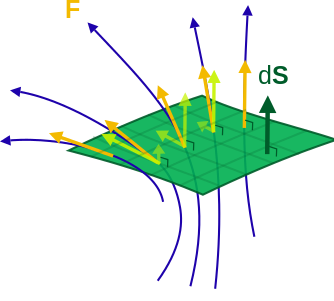
\includegraphics[width=0.400\linewidth]{flux.png}\hfill}


\chapter{Diffur- og heildareikningur vigursviða}
\label{Kafli6::doc}\label{Kafli6:diffur-og-heildareikningur-vigursvia}
\emph{A reader lives a thousand lives before he dies. The man who never reads lives only one.}

- George R.R. Martin, A Dance with Dragons


\section{grad, div og curl}
\label{Kafli6:grad-div-og-curl}

\subsection{Skilgreining}
\label{Kafli6:skilgreining}
Skilgreinum \emph{nabla}-virkjann sem diffurvirkja
\begin{gather}
\begin{split}\displaystyle \nabla=\mbox{${\bf i}$}\,\frac{\partial}{\partial x}+\mbox{${\bf j}$}\,\frac{\partial}{\partial y}+\mbox{${\bf k}$}\,\frac{\partial}{\partial z}.\end{split}\notag
\end{gather}

\subsection{Skilgreining}
\label{Kafli6:id1}
Látum
\(\mbox{${\bf F}$}(x,y,z)=F_1(x,y,z)\,\mbox{${\bf i}$}+F_2(x,y,z)\,\mbox{${\bf j}$}+F_3(x,y,z)\,\mbox{${\bf k}$}\)
vera vigursvið og \(\varphi(x,y,z)\) vera fall.

Skilgreinum \textit{stigul} \(\varphi\) sem vigursviðið
\begin{gather}
\begin{split}\displaystyle\end{split}\notag\\\begin{split}\mbox{${\rm\bf grad\,}$}\varphi=\nabla\varphi=\frac{\partial \varphi}{\partial x}\,\mbox{${\bf i}$}+
\frac{\partial \varphi}{\partial y}\,\mbox{${\bf j}$}+\frac{\partial \varphi}{\partial z}\,\mbox{${\bf k}$}.\end{split}\notag
\end{gather}
Skilgreinum \textit{sundurleitni} vigursviðsins
\(\mbox{${\bf F}$}\) sem
\begin{gather}
\begin{split}\displaystyle \mbox{${\rm\bf div\,}$}\mbox{${\bf F}$}=\nabla\cdot\mbox{${\bf F}$}=\frac{\partial F_1}{\partial x}+\frac{\partial F_2}{\partial y}+\frac{\partial F_3}{\partial z}.\end{split}\notag
\end{gather}
Skilgreinum \textit{rót} vigursviðsins \(\mbox{${\bf F}$}\) sem
\begin{gather}
\begin{split}\displaystyle\end{split}\notag\\\begin{split}\begin{aligned}
 \mbox{${\rm\bf curl\,}$}\mbox{${\bf F}$}&=\nabla\times\mbox{${\bf F}$}=\begin{vmatrix} \mbox{${\bf i}$}&\mbox{${\bf j}$}&\mbox{${\bf k}$}\\
 \frac{\partial} {\partial x}&\frac{\partial}{\partial y}&\frac{\partial}{\partial z}\\F_1&F_2&F_3\end{vmatrix} \\ &=\bigg(\frac{\partial F_3}{\partial y}-\frac{\partial F_2}{\partial z}\bigg)\,\mbox{${\bf i}$}+\bigg(\frac{\partial F_1}{\partial z}-\frac{\partial F_3}{\partial x}\bigg)\,\mbox{${\bf j}$}+\bigg(\frac{\partial F_2}{\partial x}-\frac{\partial F_1}{\partial y}\bigg)\,\mbox{${\bf k}$}.
 \end{aligned}\end{split}\notag
\end{gather}
\begin{notice}{warning}{Aðvörun:}
Ef \(\varphi(x,y,z)\) er fall þá er \(\nabla \varphi(x,y,z)\) stigullinn af \(\varphi(x,y,z)\) en \(\varphi(x,y,z)\nabla\) er \textit{diffurvirki}.
\end{notice}

\begin{notice}{warning}{Aðvörun:}
Sundurleitnin \(\mbox{${\rm\bf div\,}$}\mbox{${\bf F}$}\) er fall \({\mathbb  R}^3\rightarrow{\mathbb  R}\) en rótið \(\mbox{${\rm\bf curl\,}$}\mbox{${\bf F}$}\) er vigursvið \({\mathbb  R}^3\rightarrow{\mathbb  R}^3\).
\end{notice}


\subsection{Skilgreining}
\label{Kafli6:id2}
Látum
\(\mbox{${\bf F}$}(x,y)=F_1(x,y)\,\mbox{${\bf i}$}+F_2(x,y)\,\mbox{${\bf j}$}\)
vera vigursvið. Skilgreinum \textit{sundurleitni} \(\mbox{${\bf F}$}\) sem
\begin{gather}
\begin{split}\displaystyle\end{split}\notag\\\begin{split}\mbox{${\rm\bf div\,}$}\mbox{${\bf F}$}=\nabla\cdot\mbox{${\bf F}$}=\frac{\partial F_1}{\partial
  x}+\frac{\partial F_2}{\partial y}.\end{split}\notag
\end{gather}
og \textit{rót} \(\mbox{${\bf F}$}\) skilgreinum við sem
\begin{gather}
\begin{split}\displaystyle\end{split}\notag\\\begin{split}\mbox{${\rm\bf curl\,}$}\mbox{${\bf F}$}=\bigg(\frac{\partial F_2}{\partial x}-\frac{\partial
  F_1}{\partial y}\bigg)\,\mbox{${\bf k}$}.\end{split}\notag
\end{gather}

\subsection{Reiknireglur}
\label{Kafli6:reiknireglur}
Gerum ráð fyrir að \(\mbox{${\bf F}$}\) og \(\mbox{${\bf G}$}\)
séu vigursvið og \(\varphi\) og \(\psi\) föll. Gerum ráð fyrir
að þær hlutafleiður sem við þurfum að nota séu skilgreindar og
samfelldar.

(a)
\(\nabla(\varphi\psi)=\varphi\nabla\psi+\psi\nabla\varphi\).

(b)
\(\nabla\cdot(\varphi\mbox{${\bf F}$})=(\nabla\varphi)\cdot\mbox{${\bf F}$}+\varphi(\nabla\cdot\mbox{${\bf F}$})\).

(c)
\(\nabla\times(\varphi\mbox{${\bf F}$})=(\nabla\varphi)\times\mbox{${\bf F}$}+\varphi(\nabla\times\mbox{${\bf F}$})\).

(d)
\(\nabla\cdot(\mbox{${\bf F}$}\times\mbox{${\bf G}$})=(\nabla\times\mbox{${\bf F}$})\cdot\mbox{${\bf G}$}-\mbox{${\bf F}$}\cdot(\nabla\times\mbox{${\bf G}$})\).

(e)
\(\nabla\times(\mbox{${\bf F}$}\times\mbox{${\bf G}$})=(\nabla\cdot\mbox{${\bf G}$})\mbox{${\bf F}$}+(\mbox{${\bf G}$}\cdot\nabla)\mbox{${\bf F}$}-(\nabla\cdot\mbox{${\bf F}$})\mbox{${\bf G}$}-(\mbox{${\bf F}$}\cdot\nabla)\mbox{${\bf G}$}\).

(f)
\(\nabla(\mbox{${\bf F}$}\cdot\mbox{${\bf G}$})=\mbox{${\bf F}$}\times(\nabla\times \mbox{${\bf G}$})+\mbox{${\bf G}$}\times(\nabla\times \mbox{${\bf F}$})+(\mbox{${\bf F}$}\cdot\nabla)\mbox{${\bf G}$}+(\mbox{${\bf G}$}\cdot\nabla)\mbox{${\bf F}$}\).

(g)
\(\nabla\cdot(\nabla\times \mbox{${\bf F}$})=0\qquad\qquad\mbox{${\rm\bf div\,}$}\mbox{${\rm\bf curl\,}$}=0\)

(h)
\(\nabla\times(\nabla\varphi)=\mbox{${\bf 0}$}\qquad\qquad\mbox{${\rm\bf curl\,}$}\mbox{${\rm\bf grad\,}$}=\mbox{${\bf 0}$}\)

(i)
\(\nabla\times(\nabla\times \mbox{${\bf F}$})=\nabla(\nabla\cdot\mbox{${\bf F}$})-\nabla^2\mbox{${\bf F}$}\).

\index{sundurleitnilaus}\index{uppsprettulaus}\index{rótlaus}

\subsection{Skilgreining}
\label{Kafli6:id3}\label{Kafli6:index-0}
Látum \(\mbox{${\bf F}$}\) vera vigursvið skilgreint á svæði
\(D\).

(a) Vigursviðið \(\mbox{${\bf F}$}\) er sagt vera
\textit{sundurleitnilaust} eða \emph{uppsprettulaust} ef
\(\mbox{${\rm\bf div\,}$}\mbox{${\bf F}$}=0\) i öllum punktum
\(D\).

(b) Vigursviðið \(\mbox{${\bf F}$}\) er sagt vera \textit{rótlaust}
ef \(\mbox{${\rm\bf curl\,}$}\mbox{${\bf F}$}=\mbox{${\bf 0}$}\) á öllu
\(D\).

\begin{notice}{note}{Athugasemd:}
Vigursvið \(\mbox{${\bf F}$}(x,y,z)=F_1(x,y,z)\,\mbox{${\bf i}$}+F_2(x,y,z)\,\mbox{${\bf j}$}+F_3(x,y,z)\,\mbox{${\bf k}$}\) er rótlaust ef og aðeins ef
\begin{gather}
\begin{split}\displaystyle
\frac{\partial F_1}{\partial y}=
\frac{\partial F_2}{\partial x},\quad
\frac{\partial F_1}{\partial z}=
\frac{\partial F_3}{\partial x},\quad
\frac{\partial F_2}{\partial z}=
\frac{\partial F_3}{\partial y}.\end{split}\notag
\end{gather}\end{notice}


\subsection{Setning}
\label{Kafli6:setning}\begin{enumerate}
\item {} 
Rót vigursviðs er \textit{sundurleitnilaus}.

\item {} 
Stigulsvið er \textit{rótlaust}.

\end{enumerate}

\index{stjörnusvæði}

\subsection{Skilgreining}
\label{Kafli6:id4}\label{Kafli6:index-1}
Svæði \(D\) í rúmi eða plani kallast \textit{stjörnusvæði} ef til er
punktur \(P\) í \(D\) þannig að fyrir sérhvern annan punkt
\(Q\) í \(D\) þá liggur allt línustrikið á milli \(P\) og
\(Q\) í \(D\).


\subsection{Setning}
\label{Kafli6:id5}
Látum \(\mbox{${\bf F}$}\) vera samfellt diffranlegt vigursvið
skilgreint á \textit{stjörnusvæði} \(D\). Ef \(\mbox{${\bf F}$}\) er
rótlaust þá er \(\mbox{${\bf F}$}\) stigulsvið. Með öðrum orðum, ef
vigursviðið \(\mbox{${\bf F}$}\) er samfellt diffranlegt og
skilgreint á \textit{stjörnusvæði} \(D\) og uppfyllir jöfnurnar
\begin{gather}
\begin{split}\displaystyle\end{split}\notag\\\begin{split}\frac{\partial F_1}{\partial y}=
\frac{\partial F_2}{\partial x},\quad
\frac{\partial F_1}{\partial z}=
\frac{\partial F_3}{\partial x},\quad
\frac{\partial F_2}{\partial z}=
\frac{\partial F_3}{\partial y},\end{split}\notag
\end{gather}
þá er \(\mbox{${\bf F}$}\) stigulsvið.


\subsection{Setning}
\label{Kafli6:id6}
Lát \(\mbox{${\bf F}$}\) vera samfellt diffranlegt vigursvið
skilgreint á \textit{stjörnusvæði} \(D\). Ef \(\mbox{${\bf F}$}\) er
sundurleitnilaust þá er til vigursvið \(\mbox{${\bf G}$}\) þannig að
\(\mbox{${\bf F}$}=\mbox{${\rm\bf curl\,}$}\mbox{${\bf G}$}\).
Vigursviðið \(\mbox{${\bf G}$}\) kallast \emph{vigurmætti} fyrir
\(\mbox{${\bf F}$}\).

\index{sundurleitnisetning}

\section{Sundurleitnisetningin I}
\label{Kafli6:sundurleitnisetningin-i}\label{Kafli6:index-2}

\subsection{Setning (Sundurleitnisetning I)}
\label{Kafli6:setning-sundurleitnisetning-i}
Látum \(\mbox{${\bf F}$}\) vera samfellt diffranlegt vigursvið
skilgreint á opnu mengi \(D\) í \({\mathbb  R}^3\). Látum
\(P\) vera punkt á skilgreiningarsvæði \(\mbox{${\bf F}$}\) og
\({\cal S}_\varepsilon\) kúluskel með miðju í \(P\) og geisla
\(\varepsilon\). Látum svo \(\mbox{${\bf N}$}\) vera
einingarþvervigrasvið á \({\cal S}_\varepsilon\) þannig að
\(\mbox{${\bf N}$}\) vísar út á við. Þá er
\begin{gather}
\begin{split}\displaystyle\end{split}\notag\\\begin{split}\mbox{${\rm\bf div\,}$}\mbox{${\bf F}$}(P)=\lim_{\varepsilon\rightarrow 0^+}
\frac{1}{V_\varepsilon}\int\!\!\!\int_{{\cal S}_\varepsilon}\mbox{${\bf F}$}\cdot\mbox{${\bf N}$}\,dS.\end{split}\notag
\end{gather}
þar sem \(V_\varepsilon= 4\pi\varepsilon^3/3\) er rúmmálið innan í
\({\cal S}_\varepsilon\).

\index{Stoke!setning}

\subsection{Setning (Setning Stokes I)}
\label{Kafli6:setning-setning-stokes-i}\label{Kafli6:index-3}
Látum \(\mbox{${\bf F}$}\) vera samfellt diffranlegt vigursvið
skilgreint á opnu mengi \(D\) í \({\mathbb  R}^3\). Látum
\(P\) vera punkt á skilgreiningarsvæði \(\mbox{${\bf F}$}\) og
\(C_\varepsilon\) vera hring með miðju í \(P\) og geisla
\(\varepsilon\). Látum \(\mbox{${\bf N}$}\) vera
einingarþvervigur á planið sem hringurinn liggur í. Áttum hringinn
jákvætt. Þá er
\begin{gather}
\begin{split}\displaystyle\end{split}\notag\\\begin{split}\mbox{${\bf N}$}\cdot\mbox{${\rm\bf curl\,}$}\mbox{${\bf F}$}(P)=\lim_{\varepsilon\rightarrow 0^+}
\frac{1}{A_\varepsilon}\oint_{C_\varepsilon}\mbox{${\bf F}$}\cdot d\mbox{${\bf r}$}.\end{split}\notag
\end{gather}
þar sem \(A_\varepsilon= \pi\varepsilon^2\) er flatarmálið sem
afmarkast af \({\cal C}_\varepsilon\).


\subsection{Túlkun}
\label{Kafli6:tulkun}
Hugsum \(\mbox{${\bf F}$}\) sem lýsingu á vökvastreymi í
\({\mathbb  R}^3\).

\(\mbox{${\rm\bf div\,}$}\mbox{${\bf F}$}(P)\) lýsir því hvort
vökvinn er að þenjast út eða dragast saman í punktinum \(P\).
Sundurleitnisetningin (næsti fyrirlestur) segir að samanlögð útþensla á
rúmskika \(R\) er jöfn streymi út um jaðar svæðisins
\(\mathcal{S}\), eða
\begin{gather}
\begin{split}\displaystyle \int\!\!\!\int\!\!\!\int_R\mbox{${\rm\bf div\,}$}\mbox{${\bf F}$}\,dV=\int\!\!\!\int_{\mathcal{S}} \mbox{${\bf F}$}\cdot\mbox{${\bf N}$}\,dS.\end{split}\notag
\end{gather}
\(\mbox{${\rm\bf curl\,}$}\mbox{${\bf F}$}(P)\) lýsir hringstreymi í
kringum punktinn \(P\). Setning Stokes (þar næsti fyrirlestur) segir
að samanlagt hringstreymi á fleti \(\mathcal{S}\) er jafnt
hringstreymi á jaðri flatarins, sem við táknum með \(\mathcal{C}\),
eða
\begin{gather}
\begin{split}\displaystyle \int\!\!\!\int_{\cal S} \mbox{${\rm\bf curl\,}$}\mbox{${\bf F}$}\cdot\mbox{${\bf N}$}\,dS=\oint_\mathcal{C} \mbox{${\bf F}$}\cdot d\mbox{${\bf r}$}.\end{split}\notag
\end{gather}

\subsection{Skilgreining}
\label{Kafli6:id7}
Látum \(R\) vera svæði í \({\mathbb  R}^2\) og \(\cal C\)
\textit{jaðar} \(R\). Gerum ráð fyrir að \(\cal C\) samanstandi af endanlega mörgum ferlum \({\cal C}_1, \ldots, {\cal C}_n\). Jákvæð
\textit{áttun} á ferlunum felst í því að velja fyrir hvert \(i\) stikun \(\mbox{${\bf r}$}_i\) á \({\cal C}_i\) þannig að ef labbað eftir \({\cal C}_i\) í stefnu stikunar þá er \(R\) á vinstri hönd.

\index{Green!setning}

\subsection{Setning Green}
\label{Kafli6:index-4}\label{Kafli6:setning-green}
Látum \(R\) vera svæði í planinu þannig að jaðar \(R\), táknaður
með \(\cal C\), samanstendur af endanlega mörgum samfellt
diffranlegum ferlum. Áttum \(\cal C\) jákvætt. Látum
\(\mbox{${\bf F}$}(x,y)=F_1(x,y)\,\mbox{${\bf i}$}+F_2(x,y)\,\mbox{${\bf j}$}\)
vera samfellt diffranlegt vigursvið skilgreint á \(R\). Þá er
\begin{gather}
\begin{split}\displaystyle\end{split}\notag\\\begin{split}\oint_{\cal C}F_1(x,y)\,dx+F_2(x,y)\,dy=\int\!\!\!\int_R
\frac{\partial  F_2}{\partial x}-
\frac{\partial  F_1}{\partial y}\,dA.\end{split}\notag
\end{gather}

\subsection{Fylgisetning}
\label{Kafli6:fylgisetning}
Látum \(R\) vera svæði í planinu þannig að jaðar \(R\) táknaður
með \(\cal C\), samanstendur af endanlega mörgum samfellt
diffranlegum ferlum. Áttum \(\cal C\) jákvætt. Þá er
\begin{gather}
\begin{split}\displaystyle\end{split}\notag\\\begin{split}\mbox{Flatarmál } R=\oint_{\cal C}x\,dy=
-\oint_{\cal C}y\,dx=\frac{1}{2}\oint_{\cal C}x\,dy-y\,dx.\end{split}\notag
\end{gather}

\subsection{Sundurleitnisetningin í tveimur víddum}
\label{Kafli6:sundurleitnisetningin-i-tveimur-viddum}
Látum \(R\) vera svæði í planinu þannig að jaðar \(R\), táknaður
með \(\cal C\), samanstendur af endanlega mörgum samfellt
diffranlegum ferlum. Látum \(\mbox{${\bf N}$}\) tákna
einingarþvervigrasvið á \(\cal C\) þannig að
\(\mbox{${\bf N}$}\) vísar út úr \(R\). Látum
\(\mbox{${\bf F}$}(x,y)=F_1(x,y)\,\mbox{${\bf i}$}+F_2(x,y)\,\mbox{${\bf j}$}\)
vera samfellt diffranlegt vigursvið skilgreint á \(R\). Þá er
\begin{gather}
\begin{split}\displaystyle \int\!\!\!\int_R\mbox{${\rm\bf div\,}$}\mbox{${\bf F}$}\,dA=\oint_{\cal C} \mbox{${\bf F}$}\cdot\mbox{${\bf N}$}\,ds.\end{split}\notag
\end{gather}

\section{Sundurleitnisetningin II}
\label{Kafli6:sundurleitnisetningin-ii}
\index{flötur!reglulegur}

\subsection{Skilgreining}
\label{Kafli6:index-5}\label{Kafli6:id8}
Flötur er sagður reglulegur ef hann hefur \textit{snertiplan} í hverjum punkti.

Flötur \(\cal S\) sem er búinn til með því að taka endanlega marga
reglulega fleti \({\cal S}_1, \ldots, {\cal S}_n\) og líma þá saman
á jöðrunum kallast \emph{reglulegur á köflum}.

Þegar talað um einingarþvervigrasvið á slíkan flöt þá er átt við
vigursvið sem er skilgreint á fletinum nema í þeim punktum þar sem
fletir \({\cal S}_i\) og \({\cal S}_j\) hafa verið límdir saman.
Í slíkum punktum þarf flöturinn ekki að hafa snertiplan og því ekki
heldur þvervigur.

Flötur er sagður \emph{lokaður} ef hann er yfirborð svæðis í
\({\mathbb  R}^3\) (t.d. er kúluhvel lokaður flötur).


\subsection{Setning (Sundurleitnisetningin, Setning Gauss)}
\label{Kafli6:setning-sundurleitnisetningin-setning-gauss}
Látum \(\cal S\) vera lokaðan flöt sem er reglulegur á köflum.
Táknum með \(D\) rúmskikann sem \(\cal S\) umlykur. Látum
\(\mbox{${\bf N}$}\) vera einingarþvervigrasvið á \(\cal S\) sem
vísar út úr \(D\). Ef \(\mbox{${\bf F}$}\) er samfellt
diffranlegt vigursvið skilgreint á \(D\) þá er
\begin{gather}
\begin{split}\displaystyle \int\!\!\!\int\!\!\!\int_D \mbox{${\rm\bf div\,}$}\mbox{${\bf F}$}\,dV=\int\!\!\!\int_{\cal S} \mbox{${\bf F}$}\cdot\mbox{${\bf N}$}\,dS.\end{split}\notag
\end{gather}

\subsection{Skilgreining}
\label{Kafli6:id9}
Látum \(D\) vera rúmskika í \({\mathbb  R}^3\). Segjum að
rúmskikinn \(D\) sé \(z\)-\emph{einfaldur} ef til er svæði
\(D_z\) í planinu og samfelld föll \(f\) og \(g\) skilgreind
á \(D_z\) þannig að
\begin{gather}
\begin{split}\displaystyle D=\{(x,y,z)\mid (x,y)\in D_z\mbox{ og }f(x,y)\leq z\leq g(x,y)\}.\end{split}\notag
\end{gather}
Það að rúmskiki sé \(x\)- eða \(y\)-einfaldur er skilgreint á
sama hátt.


\subsection{Setning}
\label{Kafli6:id10}
Látum \(\cal S\) vera lokaðan flöt sem er reglulegur á köflum.
Táknum með \(D\) rúmskikann sem \(\cal S\) umlykur. Látum
\(\mbox{${\bf N}$}\) vera einingarþvervigrasvið á \(\cal S\) sem
vísar út úr \(D\). Ef \(\mbox{${\bf F}$}\) er samfellt
diffranlegt vigursvið skilgreint á \(D\) og \(\varphi\)
diffranlegt fall skilgreint á \(D\) þá er
\begin{gather}
\begin{split}\displaystyle \int\!\!\!\int\!\!\!\int_D\mbox{${\rm\bf curl\,}$}\mbox{${\bf F}$}\,dV=-\int\!\!\!\int_{\cal S}\mbox{${\bf F}$}\times\mbox{${\bf N}$}\,dS,\end{split}\notag
\end{gather}
og
\begin{gather}
\begin{split}\displaystyle \int\!\!\!\int\!\!\!\int_D\mbox{${\rm\bf grad\,}$}\varphi\,dV=\int\!\!\!\int_{\cal S}\varphi\mbox{${\bf N}$}\,dS.\end{split}\notag
\end{gather}
Athugið að útkomurnar úr heildunum eru vigrar.


\section{Setning Stokes}
\label{Kafli6:setning-stokes}

\subsection{Skilgreining}
\label{Kafli6:id11}
Látum \(\cal S\) vera áttanlegan flöt sem er reglulegur á köflum með
jaðar \(\cal C\) og einingarþvervigrasvið \(\mbox{${\bf N}$}\).
Áttun \(\cal C\) út frá \(\mbox{${\bf N}$}\) finnst með að hugsa
sér að gengið sé eftir \(\cal C\) þannig að skrokkurinn vísi í
stefnu \(\mbox{${\bf N}$}\) og göngustefnan sé valin þannig að
flöturinn sé á vinstri hönd.


\subsection{Setning (Setning Stokes)}
\label{Kafli6:setning-setning-stokes}
Látum \(\cal S\) vera áttanlegan flöt sem er reglulegur á köflum og
látum \(\mbox{${\bf N}$}\) tákna einingarþvervigrasvið á
\(\cal S\). Táknum með \(\cal C\) jaðar \(\cal S\) og áttum
\(\cal C\) með tilliti til \(\mbox{${\bf N}$}\). Ef
\(\mbox{${\bf F}$}\) er samfellt diffranlegt vigursvið skilgreint á
\textit{opnu mengi} sem inniheldur \(\cal S\) þá er
\begin{gather}
\begin{split}\displaystyle \int\!\!\!\int_{\cal S} \mbox{${\rm\bf curl\,}$}\mbox{${\bf F}$}\cdot\mbox{${\bf N}$}\,dS=\oint_{\cal C}\mbox{${\bf F}$}\cdot \mbox{${\bf T}$}\,ds.\end{split}\notag
\end{gather}

\subsection{Setning}
\label{Kafli6:id12}
Látum \(\mbox{${\bf F}$}\) vera samfellt diffranlegt vigursvið
skilgreint á opnu mengi \(D\) í \({\mathbb  R}^3\). Látum
\(P\) vera punkt á skilgreiningarsvæði \(\mbox{${\bf F}$}\) og
\(C_\varepsilon\) vera hring með miðju í \(P\) og geisla
\(\varepsilon\). Látum \(\mbox{${\bf N}$}\) vera
einingarþvervigur á planið sem hringurinn liggur í. Áttum hringinn
jákvætt. Þá er
\begin{gather}
\begin{split}\displaystyle\end{split}\notag\\\begin{split}\mbox{${\bf N}$}\cdot\mbox{${\rm\bf curl\,}$}\mbox{${\bf F}$}(P)=\lim_{\varepsilon\rightarrow 0^+}
\frac{1}{\pi\varepsilon^2}\oint_{C_\varepsilon}\mbox{${\bf F}$}\cdot d\mbox{${\bf r}$}.\end{split}\notag
\end{gather}

\subsection{Setning}
\label{Kafli6:id13}
Látum \(\cal S\) vera lokaðan flöt sem er reglulegur á köflum.
Táknum með \(D\) rúmskikann sem \(\cal S\) umlykur. Látum
\(\mbox{${\bf N}$}\) vera einingarþvervigrasvið á \(\cal S\) sem
vísar út úr \(D\). Ef \(\mbox{${\bf F}$}\) er samfellt
diffranlegt vigursvið skilgreint á opnu mengi sem inniheldur \(D\),
þá er
\begin{gather}
\begin{split}\displaystyle \oint_{\cal S}\mbox{${\rm\bf curl\,}$}\mbox{${\bf F}$}\cdot\mbox{${\bf N}$}\,dS=0.\end{split}\notag
\end{gather}

\section{Hagnýtingar í eðlisfræði}
\label{Kafli6:hagnytingar-i-elisfraei}

\subsection{Vökvaflæði}
\label{Kafli6:vokvaflaei}
Skoðum vökvaflæði í rúmi. Hugsum okkur að vökvaflæðið sé líka háð tíma.
Látum \(\mbox{${\bf v}$}(x,y,z,t)\) tákna hraðavigur agnar sem er í
punktinum \((x,y,z)\) á tíma \(t\). Látum
\(\delta(x,y,z,t)\) tákna efnisþéttleika (massi per rúmmálseiningu)
í punktum \((x,y,z)\) á tíma \(t\). Þá gildir að
\begin{gather}
\begin{split}\displaystyle \frac{\partial \delta}{\partial t}+\mbox{${\rm\bf div\,}$}(\delta\mbox{${\bf v}$})=0.\end{split}\notag
\end{gather}
(Þessi jafna kallast samfelldnijafnan um vökvaflæðið.)


\subsection{Vökvaflæði}
\label{Kafli6:id14}
Til viðbótar við \(\mbox{${\bf v}$}\) og \(\delta\) þá
skilgreinum við \(p(x,y,z,t)\) sem þrýsting og
\(\mbox{${\bf F}$}\) sem utanaðkomandi kraft, gefinn sem kraftur per
massaeiningu. Þá gildir að
\begin{gather}
\begin{split}\displaystyle \delta\frac{\partial \mbox{${\bf v}$}}{\partial t}+\delta(\mbox{${\bf v}$}\cdot\nabla)\mbox{${\bf v}$}=-\nabla p+\delta\mbox{${\bf F}$}.\end{split}\notag
\end{gather}
(Þessi jafna er kölluð hreyfijafna flæðisins.)


\subsection{Rafsvið - Lögmál Coulombs}
\label{Kafli6:rafsvi-logmal-coulombs}
Látum punkthleðslu \(q\) vera í punktinum
\(\mbox{${\bf s}$}=\xi\,\mbox{${\bf i}$}+\eta\,\mbox{${\bf j}$}+\zeta\,\mbox{${\bf k}$}\).
Í punktum
\(\mbox{${\bf r}$}=x\,\mbox{${\bf i}$}+y\,\mbox{${\bf j}$}+z\,\mbox{${\bf k}$}\)
er rafsviðið vegna þessarar hleðslu
\begin{gather}
\begin{split}\displaystyle \mbox{${\bf E}$}(\mbox{${\bf r}$})=\frac{q}{4\pi\varepsilon_0}\frac{\mbox{${\bf r}$}-\mbox{${\bf s}$}}{|\mbox{${\bf r}$}-\mbox{${\bf s}$}|^3}\end{split}\notag
\end{gather}
þar sem \(\varepsilon_0\) er \emph{r}afsvörunarstuðull tómarúms.


\subsection{Rafsvið - Lögmál Gauss (fyrsta jafna Maxwells)}
\label{Kafli6:rafsvi-logmal-gauss-fyrsta-jafna-maxwells}
Látum \(\rho(\xi,\eta,\zeta)\) vera hleðsludreifingu og
\(\mbox{${\bf E}$}\) rafsviðið vegna hennar. Þá gildir að
\begin{gather}
\begin{split}\displaystyle \mbox{${\rm\bf div\,}$}\mbox{${\bf E}$}=\frac{\rho}{\varepsilon_0}.\end{split}\notag
\end{gather}

\subsection{Rafsvið}
\label{Kafli6:rafsvi}
Látum \(\rho(\xi,\eta,\zeta)\) vera hleðsludreifingu á takmörkuðu
svæði \(R\) og \(\mbox{${\bf E}$}\) rafsviðið vegna hennar. Ef
við setjum
\begin{gather}
\begin{split}\displaystyle \varphi(\mbox{${\bf r}$}) = -\frac{1}{4 \pi \varepsilon_0} \iiint_R \frac{\rho(\mbox{${\bf s}$})}{|\mbox{${\bf r}$}-\mbox{${\bf s}$}|} dV\end{split}\notag
\end{gather}
þá er \(\mbox{${\bf E}$}= \nabla \varphi\) og þar með er
\begin{gather}
\begin{split}\displaystyle \mbox{${\rm\bf curl\,}$}\mbox{${\bf E}$}= \mathbf{0}.\end{split}\notag
\end{gather}

\subsection{Segulsvið - Lögmál Biot-Savart}
\label{Kafli6:segulsvi-logmal-biot-savart}
Látum straum \(I\) fara eftir ferli \(\cal F\). Táknum
segulsviðið með \(\mbox{${\bf H}$}\) og látum
\(\mbox{${\bf s}$}=\xi\,\mbox{${\bf i}$}+\eta\,\mbox{${\bf j}$}+\zeta\,\mbox{${\bf k}$}\)
vera punkt á ferlinum \(\cal F\). Þá gefur örbútur
\(d\mbox{${\bf s}$}\) úr \(\cal F\) af sér segulsvið
\begin{gather}
\begin{split}\displaystyle d\mbox{${\bf H}$}(\mbox{${\bf r}$})=\frac{\mu_0 I}{4\pi}\frac{d\mbox{${\bf s}$}\times(\mbox{${\bf r}$}-\mbox{${\bf s}$})}{|\mbox{${\bf r}$}-\mbox{${\bf s}$}|^3}\end{split}\notag
\end{gather}
þar sem \(\mu_0\) er \emph{s}egulsvörunarstuðull tómarúms. Af þessu
sést að
\begin{gather}
\begin{split}\displaystyle\end{split}\notag\\\begin{split}\mbox{${\bf H}$}=\frac{\mu_0 I}{4\pi}\oint_{\cal F}
\frac{d\mbox{${\bf s}$}\times(\mbox{${\bf r}$}-\mbox{${\bf s}$})}{|\mbox{${\bf r}$}-\mbox{${\bf s}$}|^3}\end{split}\notag
\end{gather}
og sýna má að ef \(\mbox{${\bf r}$}\notin \mathcal{F}\) þá er
\begin{gather}
\begin{split}\displaystyle \mbox{${\rm\bf curl\,}$}\mbox{${\bf H}$}= \mathbf{0}.\end{split}\notag
\end{gather}

\subsection{Segulsvið - Lögmál Ampére}
\label{Kafli6:segulsvi-logmal-ampere}
Hugsum okkur að straumur \(I\) fari upp eftir \(z\)-ás. Táknum
með \(\mbox{${\bf H}$}\) segulsviðið og
\(H=|\mbox{${\bf H}$}|\). Í punkti
\(\mbox{${\bf r}$}=x\,\mbox{${\bf i}$}+y\,\mbox{${\bf j}$}+z\,\mbox{${\bf k}$}\)
í fjarlægð \(a\) frá \(z\)-ás er
\(H=\frac{\mu_0 I}{2\pi a}\) og ef \(\cal C\) er lokaður
einfaldur ferill sem fer rangsælis einu sinni umhverfis \(z\)-ásinn
þá er
\begin{gather}
\begin{split}\displaystyle \oint_{\cal C} \mbox{${\bf H}$}\cdot d\mbox{${\bf r}$}=\mu_0 I.\end{split}\notag
\end{gather}
Hugsum okkur að \(\mathbf{J}(\mbox{${\bf r}$})\) sé straumþéttleiki
í punkti \(\mbox{${\bf r}$}\) (straumur á flatareiningu). Þá er
\begin{gather}
\begin{split}\displaystyle \mbox{${\rm\bf curl\,}$}\mbox{${\bf H}$}= \mu_0 \mathbf{J}.\end{split}\notag
\end{gather}
Einnig gildir að ef við setjum
\begin{gather}
\begin{split}\displaystyle\end{split}\notag\\\begin{split}\mbox{${\bf A}$}(\mbox{${\bf r}$})=\frac{\mu_0}{4\pi}\iiint_{R}
\frac{\mathbf{J}(\mathbf{s})}{|\mbox{${\bf r}$}-\mbox{${\bf s}$}|}dV,\end{split}\notag
\end{gather}
þá er \(\mbox{${\bf H}$}=\mbox{${\rm\bf curl\,}$}\mbox{${\bf A}$}\)
og því er
\begin{gather}
\begin{split}\displaystyle \mbox{${\rm\bf div\,}$}\mbox{${\bf H}$}=0.\end{split}\notag
\end{gather}

\subsection{Samantekt}
\label{Kafli6:samantekt}\begin{gather}
\begin{split}\displaystyle\end{split}\notag\\\begin{split}\begin{aligned}
  \mbox{${\rm\bf div\,}$}\mbox{${\bf E}$}&= \frac{\rho}{\varepsilon_0} \quad~ \mbox{${\rm\bf div\,}$}\mbox{${\bf H}$}= 0 \\
  \mbox{${\rm\bf curl\,}$}\mbox{${\bf E}$}&= \mathbf{0} \qquad \mbox{${\rm\bf curl\,}$}\mbox{${\bf H}$}= \mu_0 \mathbf{J}
 \end{aligned}\end{split}\notag
\end{gather}
Jöfnur Maxwells
\begin{gather}
\begin{split}\displaystyle\end{split}\notag\\\begin{split}\begin{aligned}
  \mbox{${\rm\bf div\,}$}\mbox{${\bf E}$}&= \frac{\rho}{\varepsilon_0} \qquad ~ \mbox{${\rm\bf div\,}$}\mbox{${\bf H}$}= 0 \\
  \mbox{${\rm\bf curl\,}$}\mbox{${\bf E}$}&= -\frac{\partial \mbox{${\bf H}$}}{\partial t} \quad \mbox{${\rm\bf curl\,}$}\mbox{${\bf H}$}= \mu_0 \mathbf{J} + \mu_0 \varepsilon_0  \frac{\partial\mbox{${\bf E}$}}{\partial t}
 \end{aligned}\end{split}\notag
\end{gather}
\emph{My old grandmother always used to say, Summer friends will melt away like summer snows, but winter friends are friends forever.}

- George R.R. Martin, A Feast for Crows


\chapter{Viðauki}
\label{vidauki::doc}\label{vidauki:viauki}

\bigskip\hrule{}\bigskip



\section{Kennsluáætlun}
\label{vidauki:kennsluaaetlun}


\begin{center}
\begin{tabular}{l|l|l|l}
Dags. &Efni & Nótur &Adams Calculus\\
\hline
09.01.17.&1. Ferlar.&    1.1-1.5.     &8.1, {\bf 8.2}, {\bf 8.3}, {\bf 8.4},\\
&&&{\bf 11.1}, 11.2, {\bf 11.3}.\\
&Viðbótarefni:  Krossmargfeldi& {\bf 10.3}.\\
11.01.17.&2. Ferlar í plani og pólhnit.& 1.6-1.10.& {\bf 8.4}, {\bf 8.5}, {\bf 8.6}.\\
\hline
16.01.17.&3. Krappi og vindingur.& 1.10-1.17.& {\bf 11.4}, {\bf 11.5}, 11.6.\\
18.01.17.&4. Föll af mörgum 
breytistærðum.\ \ \ \ \ \ & 2.1-2.10.& {\bf 12.1}, {\bf 12.2}.\\
\hline
23.01.17.&5. Hlutafleiður.& 2.11-2.13.&{\bf 12.3}, {\bf 12.4}.\\
25.01.17.&6. Keðjureglan.&2.14-2.15.&{\bf 12.5}.\\
\hline
30.01.17.&7. Línulegar nálganir.&2.16-2.25.&{\bf 12.6}\\
01.02.17.&8. Stiglar.&2.26-2.31.&{\bf 12.7}.\\
\hline
06.02.17.&9. Fólgin föll og Taylor-nálganir.&2.32.&{\bf 12.8}, {\bf 12.9}.\\
08.02.17.&10. Útgildi. &3.1-3.9.&{\bf 13.1}, {\bf 13.2}.\\
\hline
13.02.17.&11. Lagrange-margfaldarar. &3.10-3.11.&{\bf 13.2}, {\bf 13.3}.\\
15.02.17.&12. Tvöföld heildi. &4.1-4.4.&{\bf 14.1}, {\bf 14.2}, {\bf 14.3}.\\
\hline
20.02.17.&13. Meira um tvöföld heildi. &4.5-4.7.&{\bf 14.1}, {\bf 14.2}, {\bf 14.3}.\\
22.02.17.&14. Breytuskipti. &4.8.&{\bf 14.4}.\\
&  {\bf Próf úr  lesnu efni.$^\ast$}&\\
\hline
27.02.17.&15. Þreföld heildi. &4.9.& {\bf 14.5}, {\bf 14.6}.\\
01.03.17.&16. Hagnýtingar margfaldra heilda.&4.10-4.14. &{\bf 14.7}.\\
\hline
06.03.17.&17. Vigursvið og stigulsvið. &5.1-5.3.&{\bf 15.1}, {\bf 15.2}.\\
08.03.17.&18. Ferilheildi. & 5.4-5.5.&{\bf 15.3}. \\
\hline
13.03.17.&19. Ferilheildi og stigulsvið. &5.6.&{\bf 15.2}, {\bf 15.3}, {\bf 15.4}.\\
15.03.17.&20. Fletir. &5.7-5.11.&{\bf 15.5}. \\
\hline
20.03.17.&21. Flatarheildi.   &5.12.&{\bf 15.5}, {\bf 15.6}\\
22.03.17.& 22. Áttanlegir fletir. &5.13-5.15.&  {\bf 15.6}\\
&  {\bf Próf úr skiladæmum.$^\ast$} &\\
\hline
27.03.17.&  23. grad, div og curl. &6.1.&{\bf 16.1}, {\bf 16.2}.\\
29.03.17.& 24. Sundurleitnisetningin I. &6.2.&{\bf 16.2}, {\bf 16.3}, {\bf 16.4}.\\
\hline
03.04.17.&25. Sundurleitnisetningin II.&6.3& {\bf 16.2}, {\bf 16.3}, {\bf 16.4}.\\
05.06.17.&26. Setning Stokes.  &6.4.& {\bf 16.5}, {\bf 16.6}.\\
\hline
10.04.17.&27. Hagnýtingar í eðlisfræði. &6.5.& {\bf 16.6}.\\
12.04.17.& {\bf Páskafrí} & & \\
\hline
17.04.17.& {\bf Páskafrí} & & \\
19.04.17.&28. Langur dæmatími. & \\

\end{tabular}
\end{center}


Kaflanúmer í Adams Calculus miðast við 8. útgáfu kennslubókarinnar. Megináhersla er á efni þeirra kafla sem eru feitletraðir.


{\color{red}\bfseries{}*}Með fyrirvara um breyttar dagsetningar.




\end{itemize}



\renewcommand{\indexname}{Atriðaskrá}
\printindex
\end{document}
